% Copyright (C) 2007 Technical University of Liberec.  All rights reserved.
%
% Please make a following refer to Flow123d on your project site if you use the program for any purpose,
% especially for academic research:
% Flow123d, Research Centre: Advanced Remedial Technologies, Technical University of Liberec, Czech Republic
%
% This program is free software; you can redistribute it and/or modify it under the terms
% of the GNU General Public License version 3 as published by the Free Software Foundation.
%
% This program is distributed in the hope that it will be useful, but WITHOUT ANY WARRANTY;
% without even the implied warranty of MERCHANTABILITY or FITNESS FOR A PARTICULAR PURPOSE.
% See the GNU General Public License for more details.
%
% You should have received a copy of the GNU General Public License along with this program; if not,
% write to the Free Software Foundation, Inc., 59 Temple Place - Suite 330, Boston, MA 021110-1307, USA.
%
%
%
% use PDFLatex to compile this
%

\documentclass[12pt,a4paper]{report}

%%% remove comment delimiter ('%') and specify encoding parameter if required,
%%% see TeX documentation for additional info (cp1252-Western,cp1251-Cyrillic)
%\usepackage[cp1252]{inputenc}

%%% remove comment delimiter ('%') and select language if required
%\usepackage[english,spanish]{babel}
%\usepackage{czech}
\usepackage{amssymb}
\usepackage{amsmath}
\usepackage{array}
\usepackage{longtable}
\usepackage{tabularx}
\usepackage{graphicx} %[dvips]
\usepackage{etoolbox}

\usepackage{fancyvrb}	% extended verbatim environments (for examples of IO files)
\usepackage{hyperref}   % hypertext capabilities, should by last package
\hypersetup{backref,colorlinks=true}  %setup hyperef package

\newcommand{\vari}[1]{{\it #1}}
\newcommand{\ditem}[2]{\item[\vari{#1} {\tt #2}]}
\newenvironment{fileformat}{\tt\begin{flushleft}}{\end{flushleft}}
%
%% ini table environment
\newcommand{\key}[1]{{\tt #1 }}
\newcommand{\type}[1]{{\bf #1}}
%
\newenvironment{initable}[1]{%
        \vspace{4ex}
        \noindent
        Section: \textbf{[#1]}\\
        \begingroup
        %%
        %% internal commands of initable environment
        %%
       \newcommand{\br}{\hfill\break}
        %%
        \renewcommand{\arraystretch}{1.4}
        \renewcommand{\tabcolsep}{2mm}
        \small
        \baselineskip 3ex
        %\begin{longtable}{@{}lp{5cm}p{5cm}p{9cm}}%
        \tabularx{\textwidth}{l>{\centering}p{2cm}>{\raggedright}p{2cm}>{\raggedright\arraybackslash}X}%
        %\renewcommand{\\}{\\[3ex]}%
        \hline\hline
        KEY & TYPE & DEFAULT & DESCRIPTION \\%\endhead
        \hline\hline
}{%
        %\end{longtable}
        \endtabularx
        \endgroup
}

%%%%%%%%%%%%%%%%%%%% specific math macros
\def\prtl{\partial}
\def\vc#1{\mathbf{\boldsymbol{#1}}}     % vector
\def\tn#1{{\mathbb{#1}}}    % tensor
\def\abs#1{\lvert#1\rvert}
\def\Abs#1{\bigl\lvert#1\bigr\rvert}
\def\div{{\rm div}}
\def\Lapl{\Delta}
\def\grad{\nabla}

%% ini_table members

%%% remove comment delimiter ('%') and specify parameters if required
%\usepackage[dvips]{graphics}

%%%%%%%%%%%%%%%%%%%%%%%%%%%%%%%%%%%%%%%%%%%%%%%%%%%%%%%%%%%%%%%%%%%%%%%%%%%%%%%%%%%%%%%%%%%%% BEGIN DOCUMENT
%% set specific page layout
\addtolength{\textwidth}{2cm}
\addtolength{\hoffset}{-1.5cm}
\addtolength{\textheight}{4cm}
\addtolength{\voffset}{-2.5cm}
\begin{document}

%%% remove comment delimiter ('%') and select language if required
%\selectlanguage{spanish} 
\thispagestyle{empty}
\begin{center}
\noindent 
\textbf{\LARGE{
  Technical university of Liberec
}}

\vspace{2ex}
\textbf{\LARGE{
  Faculty of mechatronics, informatics\\
  and interdisciplinary studies
}}

\vspace{160pt}

\textbf{\Huge{
FLOW123D - draft, scheme of new inputs
}}

\vspace{1cm}
\textbf{\Large{
version 1.7.0
}}

\vspace{1cm}

\textbf{\Large{
Documentation of file formats \\
and brief user manual.
}}


\vspace{7cm}

\noindent \textbf{\Large{Liberec, 2011}}

\vspace{1cm}

{\bf Acknowledgement.} This work was realized under the state  subsidy of the Czech Republic within the research and development 
project ``Advanced Remediation Technologies and Processes Center'' 1M0554 
-- Program of Research Centers PP2-D01 supported by Ministry of Education.
\end{center}
\noindent 

\noindent

\tableofcontents
\pagebreak
%\setcounter{page}{2}

\parindent=0pt
\parskip=1ex

\section{}
\chapter{Quick start}

Flow123D is a software for simulation of water flow and reactionary solute transport in a heterogeneous 
porous and fractured medium. In particular it is suited for simulation of underground processes in a granite rock massive.
The program is able to describe explicitly processes in 3D medium, 2D fractures, and 1D chanels and exchange between 
domains of different dimension. The computational mesh is therefore collection of 3D tetrahedrons, 2D triangles and 1D line segments.

The water flow model assumes a saturated medium described by Darcy law. For discretization, we use lumped mixed-hybrid finite element method.
We support both steady and unsteady water flow.

The solute transport model can deal with several dissolved substances. It contains non-equilibrium dual porosity model, 
i.e. exchange between mobile and immobile 
pores. There is also model for several types of adsorption in both the mobile and immobile zone. The implemented adsorption models are
linear adsorption, Freundlich isotherm and Langmuir isotherm. The solute transport model uses finite volume discretization 
with up-winding in space and explicit Euler discretization in time. The dual porosity and the adsorption are introduced into transport by operator splitting.
The dual porosity model use analytic solution and the non-linear adsorption is solved numerically by the Newton method.

Reaction between transported substances can be modeled either by a SEMCHEM module, which is slow, but can describe all sorts of reactions. On the other hand,
for reactions of the first order, i.e. linear reactions or decays, we provide our own solver which is much faster. Reactions are coupled with transport 
by the operator splitting method,

The program provides output of the pressure, the velocity and the concentration fields in two file formats. You can use file format of GMSH mesh generator and post-processor 
or you can use output into widely supported VTK format. In particular we recommend Paraview software for visualization and post-processing of VTK data.

The program is implemented in C/C++ using essentially PETSC library for linear algebra. The water flow as well as the transport simulation and reactions can be computed 
in parallel using MPI environment. 

The program is distributed under GNU GPL v. 3 license and is available on the project web page:
http://dev.nti.tul.cz/trac/flow123d

\section{Basic usage}

\subsection{How to run the simulation.}
On the Linux system the program can be started either directly or through a script \verb'flow123d.sh'. When started directly, e.g. by the command
\begin{verbatim}
  > flow123d -s example.ini
\end{verbatim}
the program requires one argument after switch \verb'-s' which is the name of the principal input file. Full list of possible command line arguments is as follows.

\begin{description}
 \item[-s {\bf\it file}] \hfill\\
 	 Set principal INI input file. All relative paths in the INI file are relative against current directory.
 \item[-S {\bf\it file}] \hfill\\
 	Set principal INI input file. All relative paths in the INI file are relative against directory of the INI file. This is equivalent
to change directory to the directory of the INI file at the start of the program.
 \item[-i {\bf\it path}] \hfill\\
 	When there is string \verb"${INPUT}" %$
  	in the any path in the INI file, it will be replaced by given {\it path}.
 \item[-o {\bf\it path}] \hfill\\
 	Every relative path for any output file will be relative to this {\it path}. 
 \item[-l {\bf\it [file\_name]}] \hfill\\
 	Set base name of log files or turn logging off if no file name is given.

\end{description}

All other parameters will be passed to the PETSC library. An advanced user can influence lot of parameters of linear solver. In order to get list of supported options 
use parameter \verb'-help'.


Alternatively, you can use script \verb'flow123d.sh' to start parallel jobs or limit resources used by the program. This script accepts the same parameters as the program itself
and further following additional parameters:

\begin{description}
  \item[-h] \hfill\\
  	Usage overview.
  \item[-t {\bf\it timeout}] \hfill\\
  	Upper estimate for real running time of the calculation. Kill calculation after {\it timeout} seconds. 
  	Can also be used by PBS to choose appropriate job queue. 
  \item[-np {\bf\it number of processes}] \hfill\\
  	Specify number of parallel processes for calculation.
  \item[-m {\bf\it memory limit}] \hfill\\
  	Limits total available memory to {\it memory limit} bytes.
  \item[-n {\bf\it priority}] \hfill\\
  	Change (lower) priority for the calculation. See {\tt nice} command.
  \item[-r {\bf\it out file}] \hfill\\
  	Stdout and stderr will be redirected to {\it out file}.
\end{description}

On the Windows system we use Cygwin libraries in other to emulate Linux API. Therefore you have to keep the Cygwin libraries within the same direcotry as the program executable.
The Windows package that can be downloaded from project web page contains both the Cygwin libraries and the mpiexec command for starting parallel jobs on the Windows workstations.

Then you can start the sequential run by the command:
\begin{verbatim}
  > flow123d.exe -s example.ini
\end{verbatim}
or the parallel run by the command:
\begin{verbatim}
  > mpiexec.exe -np 2 flow123d.exe -s example.ini
\end{verbatim}
The program accepts the same parameters as the Linux version, but there is no script similar to \verb'flow123d.sh' for the Windows system.


\subsection{Structure of input}

The principal input file of the program is an INI file which contains names of other necessary input files.
Those are the file with calculation mesh (\verb'*.msh'), the file with specification of adjacency between dimensions (\verb'*.ngh'),
the file with material description (\verb'*.mtr') and the file with boundary conditions for the water flow problem (\verb'*.bcd').
For unsteady water flow you have to specify file with initial condition for the pressure (key \verb'Input/Initial') and optionally one can introduce 
file with water sources (key \verb'Input/Sources').

In the case of transport simulation one have to specify also the file with transport boundary conditions (\verb'*.tbc') 
and the file with transport initial condition
for individual substances (\verb'*.tic').

 \begin{figure}[h]
    \begin{center}
      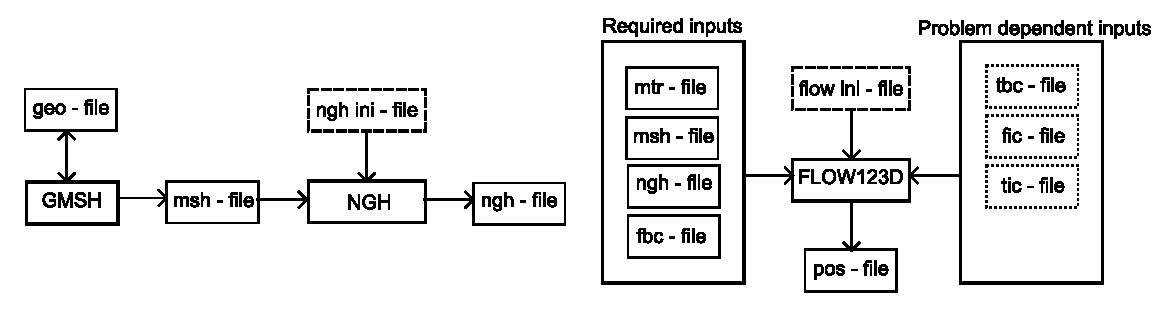
\includegraphics[scale=0.7]{schema.pdf} % 
      \caption{Preparation of input files.}
      \label{obr3}
    \end{center}
  \end{figure}


For the preparation of input files we use several utilities (see Figure \ref{obr3}). 
We usually begin with a \verb'*.geo' file as a description of the domain geometry. This come as an input for the GMSH mesh generator, which produce 
the mesh file. Then we run program \verb'ngh' to produce adjacency file. Finally we can use program \verb'bcd' for the preparation of files with
boundary and initial conditions. The file with material properties has to be created manually, preferably by modifying some of the example problems.
The programs \verb'ngh' and \verb'bcd' are distributed together with flow123d with their own limited documentation.

The output files can be either \verb'*.msh' files accepted by the GMSH or one can use VTK format that can be post-processed by Paraview.

In the following chapter, we briefly describe structure of individual input files in particular the main INI file. In the last chapter, we describe
mathematical models and numerical methods used in the Flow123d.


\chapter{Mathematical models of physical reality}

\chapter{Numerical methods}
% Copyright (C) 2007 Technical University of Liberec.  All rights reserved.
%
% Please make a following refer to Flow123d on your project site if you use the program for any purpose,
% especially for academic research:
% Flow123d, Research Centre: Advanced Remedial Technologies, Technical University of Liberec, Czech Republic
%
% This program is free software; you can redistribute it and/or modify it under the terms
% of the GNU General Public License version 3 as published by the Free Software Foundation.
%
% This program is distributed in the hope that it will be useful, but WITHOUT ANY WARRANTY;
% without even the implied warranty of MERCHANTABILITY or FITNESS FOR A PARTICULAR PURPOSE.
% See the GNU General Public License for more details.
%
% You should have received a copy of the GNU General Public License along with this program; if not,
% write to the Free Software Foundation, Inc., 59 Temple Place - Suite 330, Boston, MA 021110-1307, USA.

\normalsize
 \subsection{Advection-Diffusion equation}
 
Solute transport is governed by advection equation which can be written in the form
\begin{equation}
 \frac{\partial c}{\partial t} + \boldsymbol{v} \frac{\partial c}{\partial x}  = 0, \label{Aeq}
\end{equation}
where $c$ is concentration $[M^3 \cdot L^{-3}]$, $t$ is time $[T]$, $v$ is velocity $[L \cdot T^{-1}]$, and $x$ is coordinate in cartesian system $[L]$.
Assuming solution which is constant on every element (cell centered finite volume method) and integrating equation (\ref{Aeq}) we get
    \begin{equation}
    \int\limits_{e_i} \frac{\partial c}{\partial t} dV + \int\limits_{e_i} \boldsymbol{v} \frac{\partial c}{\partial x} \, dV = 0. \notag 
    \end{equation}
    After some rearrangements we obtain on $i$-th element ($e_i$)
    \begin{equation}
    \frac{\partial c_i}{\partial t}  V_{i} + c \int\limits_{\partial e_i }  \boldsymbol{v} \, \mathbf{dS} = 0, \label{Aeqint} 
    \end{equation}
  where $c_i$ is average concentration in $e_i$ and $V_{i}$ its volume, $c$ will be specified later (there are two main possibilities - $c_i$ or concentration from neighbouring element).
    Term $\frac{\partial c}{\partial t}$ we approximate by explicit Euler difference
    \begin{equation}
     \frac{\partial c}{\partial \textrm{t}} \approx \frac{c_{i}^{n+1} - c_{i}^n}{\Delta t}. \label{expliciteuler}
    \end{equation}
    Where $\Delta t$ is a time step and upper index at $c_i$ means values in the discrete time steps $n+1$ and $n$.
    We assume that all elements have piecewise smooth element boudary $\partial e$ with outwards directed normal. Inside the area $\Omega$ we introduce internal flows.
    With respect to $e_i$, we define internal flow intake $U_{ij}^{-}$ (from element $e_j$) and
    internal flow drain $U_{ij}^{+}$ (to element $e_j$) as follows
    \begin{eqnarray}     
      U_{ij}^{-} = \text{min}(\int\limits_{\partial e_i \cap \partial e_j, i \ne j} \boldsymbol{v} \, \mathbf{dS},0), \notag \\
      U_{ij}^{+} = \text{max}(\int\limits_{\partial e_i \cap \partial e_j, i \ne j} \boldsymbol{v} \, \mathbf{dS},0). \label{iflux}  
    \end{eqnarray}
  Those flows realizes solute transport in the area $\Omega$. On the $\partial\Omega$ we define external flows which will be important for transport Dirichlet boundary  
  conditions. In the same way as for internal flows we assume
  (with respect to element $e_i$) external flow intake $U_{ij}^{e-}$ (from $\partial\Omega$) and external flow drain $U_{ij}^{e+}$ (to $\partial\Omega$).
    \begin{eqnarray}     
      U_{ik}^{e-} = \text{min}(\int\limits_{\partial e_i \cap \partial \Omega } \boldsymbol{v} \, \mathbf{dS},0), \notag \\
      U_{ik}^{e+} = \text{max}(\int\limits_{\partial e_i \cap \partial \Omega } \boldsymbol{v} \, \mathbf{dS},0). \label{eflux}  
    \end{eqnarray}
    Direction of the velocity $\boldsymbol{v}$, which affects sign of the $U$-terms is significant for the construction solution. For the solution
    stability it is suitable to use an upwind scheme, which can by written for finite difference on simple 1D geometry in the form
    \begin{eqnarray} 
      v>0 : \frac{\partial c}{\partial \textrm{x}} \approx \frac{c_{i}^n - c_{i-1}^n}{\Delta x},   \notag \\
      v<0 : \frac{\partial c}{\partial \textrm{x}} \approx \frac{c_{i+1}^n - c_i^n}{\Delta x}.   \label{upwind} 
    \end{eqnarray}
    This scheme can be interpreted as well as in finite volume method - in convection term one can get $c$ value opposite the flow of the quantity $\boldsymbol{v}$ direction.
      For every $e_i$ we introduce itemsets $\mathcal{N}_{i}, \mathcal{B}_{i}$ which contains indexes of neighbourging elements, local boundary conditions respectivelly.  
     Assuming upwind scheme, using (\ref{iflux}), (\ref{eflux}), and  (\ref{expliciteuler}) we can write solution of the equation (\ref{Aeqint}) 
    (relation between two consecutive time steps) on $e_i$ in the form 
    \begin{equation}
      c_i^{n+1} = c_i^n - \frac{\Delta t}{V_{i}} \left[ \sum_{j \in \mathcal{N}_{i}} \left[ U_{ij}^{+} c_i +  U_{ij}^{-} c_{j} \right] +
      \sum_{k \in \mathcal{B}_{i}}  \left[  U_{ik}^{e+} c_i +  U_{ik}^{e-} c_{B_{ik}} \right] \right]. \label{Aeqsol}
    \end{equation}
    Where $c_{B_{ik}}$ are values of Dirichlet boundary conditions which belong to $e_i$. Formula (\ref{Aeqsol}) can be rewritten into the matrix notation
    \begin{equation}
     \mathbf{c}^{n+1} = (\mathbf{I} + \Delta t \mathbf{A}) \cdot \mathbf{c}^{n} + \Delta t \mathbf{B} \cdot \mathbf{c_{B}}^{n} \label{AeqsolM}
    \end{equation}
  Where $\mathbf{c}$ is vector of $c_i^{n+1}$, $\mathbf{A}$ is a square matrix composed from $\frac{U_{ij}^{+}}{V_i}$, $\frac{U_{ij}^{-}}{V_i}$, and
  $\frac{U_{ij}^{e+}}{V_i}$. $\mathbf{B}$ is in general rectangular matrix composed from $\frac{U_{ij}^{e-}}{V_i}$ and $\mathbf{c_{B}}^{n}$ is  vector of Dirichlet
  boundary conditions.matrix definition. There is one stability condition for time step which is called Courant-Friedrich-Levy condition. 
  For the problem without sources/sinks it can be written as
  \begin{equation}
  \Delta t_{max} = \min_i \left( \frac{V_i}{ \sum\limits_{j}  U_{ij}^{+} + \sum\limits_{k}  U_{ik}^{e+} } \right) =
  \min_i \left( \frac{V_i}{ \sum\limits_{j} | U_{ij}^{-} | + \sum\limits_{k} | U_{ik}^{e-} | } \right). \label{cfl} 
  \end{equation}
  This condition has a physical interpretation, which can be understood as conservation law - volume that intakes/drains to/from element $e_i$ 
can not be higher then element volume $V_i$. From algebraical point of view this condition can be seen as a condition which bounds norm of the evolution operator as follows 
  \begin{equation}
  \| \mathbf{I} + \Delta t \mathbf{A} \quad \Delta t \mathbf{B} \| \le 1.
  \end{equation}
 \subsection{Generalization}
  This approach can be used as well as for more general element connections -- for compatible/non-compatible element interconnection, if we know the flow integral
  values ($U_{ij}^{+}$ or $U_{ij}^{-}$). %Situation for more general case is in the picture (\ref{compmodel}).
      \begin{figure}[h]
        \begin{center}
        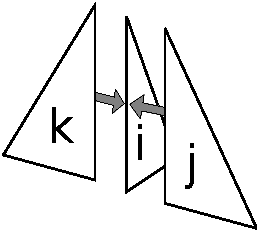
\includegraphics[scale=0.7]{obr7.pdf} 
	\caption{Edge with 3 elements}
	\label{edgemodel}
        \end{center}
      \end{figure}  
  The most general case of connection is relation among $n$ elements like in figure (\ref{edgemodel}). For this case we define
edge element indexset $\mathcal{G}_{l}$ that contains all the indexes of elements which sides make $l$-th edge ($g_l$), so that $\mathcal{G}_{l} = \{i,j,k\}$.
For $\mathcal{G}_{l}$ we introduce its subsets $\mathcal{G}_{ij}$, $\mathcal{G}_{ji}$, $\mathcal{G}_{ik}$, $\mathcal{G}_{ki}$, $\mathcal{G}_{kj}$, and $\mathcal{G}_{jk}$,
  where $\mathcal{G}_{ij} = \mathcal{G}_{ik} =  \mathcal{G}_{l} \backslash {i} = \{j,k\}$, $ \mathcal{G}_{ji} = \mathcal{G}_{jk} = \mathcal{G}_{l} \backslash {j} =\{i,k\}$, and
 $\mathcal{G}_{ki} = \mathcal{G}_{kj} = \mathcal{G}_{l} \backslash {k} =\{i,j\}$. It can be written in the same way for any edge $g$ with more than 3 elements, 
it is hold  $|\mathcal{G}_{g}| - 1 = |\mathcal{G}_{ab}|; \forall a,b \in \mathcal{G}_{g}$.
For $l$-th edge ($g_l$) we can define total edge flow $U_{g_{l}}$ eg. as
  \begin{eqnarray}
   U_{g_{l}} &=& \sum\limits_{m \in \mathcal{G}_{ji}}   \left[ U_{mj}^{+}   + \frac{ U_{jm}^{+}}{|\mathcal{G}_{ji}|} \right] = \sum\limits_{m \in \mathcal{G}_{jk}}  \left[ U_{mj}^{+}   +  \frac{ U_{jm}^{+}}{|\mathcal{G}_{jk}|} \right] \notag \\
	      &=& \sum\limits_{m \in \mathcal{G}_{ij}}  \left[ U_{mi}^{+}   +  \frac{ U_{im}^{+}}{|\mathcal{G}_{ij}|} \right] = \sum\limits_{m \in \mathcal{G}_{ik}} \left[  U_{mi}^{+} +  \frac{ U_{im}^{+}}{|\mathcal{G}_{ik}|} \right] \notag \\ 
	      &=& \sum\limits_{m \in \mathcal{G}_{ki}}  \left[ U_{mk}^{+}   +  \frac{ U_{km}^{+}}{|\mathcal{G}_{ki}|} \right] = \sum\limits_{m \in \mathcal{G}_{kj}}  \left[ U_{mk}^{+}   +  \frac{ U_{km}^{+}}{|\mathcal{G}_{kj}|} \right], \label{edgeflow}
  \end{eqnarray}
$U_{g_{l}}$ with respect to any $e_m$; $m \in \mathcal{G}_{l}$ has to have the same value because continuity equation, for assumed incompresible flow, has to
 be fulfilled in every edge. Edges with more than two elements and two and more nonzero intakes to edge realize an ideal mixing (to an average concentration) 
with weights which will be specified later. This fact modifies equation (\ref{Aeqsol}) on the general mesh into the form
    \begin{equation}
      c_i^{n+1} = c_i^n - \frac{\Delta t}{V_{i}} \left[ \sum_{j \in \mathcal{N}_{i}} \left[ U_{ij}^{+} c_i +  \frac{U_{ij}^{-}}{ \sum\limits_{k \in \mathcal{G}_{ij}}
      \left[ U_{ki}^{+} + \frac{U_{ik}^{+}}{|\mathcal{G}_{ij}|} \right] } \sum\limits_{k \in \mathcal{G}_{ij}} U_{ki}^{+} c_{k} \right] + 
      \sum_{k \in \mathcal{B}_{i}}  \left[  U_{ik}^{e+} c_i +  U_{ik}^{e-} c_{B_{ik}} \right] \right]. \label{Aeqsol2}
    \end{equation}
The edges with total edge flow $U_{g_{l}} = 0$ can occur breakdown in the equation (\ref{Aeqsol2}) via term $\sum\limits_{k \in \mathcal{G}_{ij}}\left[ U_{ki}^{+} + \frac{U_{ik}^{+}}{|\mathcal{G}_{ij}|} \right] = 0$.
This fact implies as well as numerator $U_{ij}^{-} = 0$. In order to avoid dividing by zero we have to assume computation only for nonzero flows.
Concentrations $c_k$, $k \in \mathcal{G}_{ij}$ that may intakes into element $e_i$ are weighted with weights 
\begin{equation}
 \alpha_k = \frac{U_{ki}^{+}}{\sum\limits_{k \in \mathcal{G}_{ij}} \left[ U_{ki}^{+} + \frac{U_{ik}^{+}}{|\mathcal{G}_{ij}|} \right] }, \label{weights}
\end{equation}
so that the ideal mixing in this edge leads to the average concentration 
\begin{equation}
 c_{av} = \frac{\sum\limits_{k \in \mathcal{G}_{ij}} U_{ki}^{+} c_{k}}{\sum\limits_{k \in \mathcal{G}_{ij}} \left[ U_{ki}^{+} + \frac{U_{ik}^{+}}{|\mathcal{G}_{ij}|} \right] }. \label{cav}
\end{equation}
Matrix notation is the same as in (\ref{AeqsolM}). Finally ...

% Copyright (C) 2007 Technical University of Liberec.  All rights reserved.
%
% Please make a following refer to Flow123d on your project site if you use the program for any purpose,
% especially for academic research:
% Flow123d, Research Centre: Advanced Remedial Technologies, Technical University of Liberec, Czech Republic
%
% This program is free software; you can redistribute it and/or modify it under the terms
% of the GNU General Public License version 3 as published by the Free Software Foundation.
%
% This program is distributed in the hope that it will be useful, but WITHOUT ANY WARRANTY;
% without even the implied warranty of MERCHANTABILITY or FITNESS FOR A PARTICULAR PURPOSE.
% See the GNU General Public License for more details.
%
% You should have received a copy of the GNU General Public License along with this program; if not,
% write to the Free Software Foundation, Inc., 59 Temple Place - Suite 330, Boston, MA 021110-1307, USA.

\normalsize

%%%%%%%%%%%%%%%%%        DOCUMENTATION OF GENERAL KINETIC REACTION FOR FUTURE -START           %%%%%%%%%%%%%%%

% \subsection{General Kinetic Reaction}
% \label{sec:kinetic}
% We consider a system of $m$ stoichiometric reactions, each symbolically written as
% \begin{equation} \label{eqn:general_kinetic_reaction}
%   \sum\limits_{i=1}^{n_r} \nu_{rik}\chi_{i} \rightarrow \sum\limits_{i=1}^{n_r} \nu_{pik} \chi_{i},
% \end{equation}
% where 
% \begin{itemize}
%   \item $\nu_{rik}$ \units{}{}{} is the stoichiometric coefficient (number of moles) 
%         for reactant component $i$ in reaction $k$,
%   \item $\nu_{pik}$ \units{}{}{} is the stoichiometric coefficient
%         for product component $i$ in reaction $k$,
%   \item $n_r$ is the number of reaction components (both reactants and products),
%   \item $\chi_{i}$ represents the chemical symbol for the component $i$.
% \end{itemize}
% For the components that are not present in reaction, the stoichiometric coefficients are set
% $\nu_{rik}=0$ or $\nu_{pik}=0$.
% 
% The kinetics temperature dependence is introduce in modified Arrhenius model.
% The production rate of the component $i$ is then modeled as
% \begin{equation} \label{eqn:modified_arrhenius}
%   \frac{\d c_i}{\d t} = M_i \sum\limits_{k=1}^{m}\left( \nu_{pik}-\nu_{rik} \right) 
%   B_k \left(\frac{T}{T_{0k}}\right)^{\alpha_k} \exp\left(-\frac{\Delta E_k}{R_gT}\right)
%   \prod\limits_{j=1}^{n_r}\left(\frac{\rho_j}{M_j}\right)^{\nu_{rjk}},
% \end{equation}
% where
% \begin{itemize}
%   \item $c_i$ \units{1}{-3}{} is concentration of component $i$,
%   \item $M_i$, $M_j$ \units{1}{-3}{} is the molar mass of component $i$, or $j$ respectively,
%   \item $B_k$ \units{}{}{-1} is the collision-frequency factor (or preexponential factor) of reaction $k$,
%               it represents number of all particle collisions per second (not all necessarilly 
%               resulting in reaction),
%   \item $T$ [K] is the current absolute temperature,
%   \item $T_{0k}$ [K] is the reference absolute temperature, at which the number of particle collisions per second
%         is equal $B_k$,
%   \item $\alpha_k$ \units{}{}{} is the temperature exponent of the reaction $k$,
%   \item $\Delta E_k$ $[\textrm{Jmol}^{-1}]$ is the activation energy per mole,
%   \item $R_g = 8.3144$ $[\textrm{Jmol}^{-1}\textrm{K}^{-1}]$ is the universal gas constant,
%   \item $\rho_j$ \units{1}{-3}{} is the density of component $j$.
% \end{itemize}
% 
% To get rid of the unit dependence on the exponent, we divide the equation \eqref{eqn:modified_arrhenius} 
% by liquid density $\rho=\sum_{j=1}^{n_r}\rho_i$ and put $M_i$ under the exponent. Using
% \begin{equation}
%   \prod\limits_{j=1}^{n_r}\left( \frac{\rho_j M_i}{\rho M_j}\right)^{\nu_{rjk}} 
%   = \left(\frac{M_i}{\rho}\right)^{\sum_{j=1}^{n_r}\nu_{rjk}} 
%     \prod\limits_{j=1}^{n_r}\left( \frac{\rho_j}{M_j}\right),
% \end{equation}
% we obtain
% \begin{equation}
%   \frac{\d}{\d t}\left(\frac{c_i}{\rho}\right) = \sum\limits_{k=1}^{m}\left( \nu_{pik}-\nu_{rik} \right) 
%   B_k \left(\frac{T}{T_{0k}}\right)^{\alpha_k} \exp\left(-\frac{\Delta E_k}{R_gT}\right)
%   \left(\frac{M_i}{\rho}\right)^{1-\sum_{j=1}^{n_r}\nu_{rjk}} 
%   \prod\limits_{j=1}^{n_r}\left( \frac{\rho_j M_i}{\rho M_j}\right)^{\nu_{rjk}} 
% %   
% %   = \left(\frac{M_i}{\rho}\right)^{\sum_{j=1}^{n_r}\nu_{rjk}} 
% %     \prod\limits_{j=1}^{n_r}\left( \frac{\rho_j}{M_j}\right),
% \end{equation}

%%%%%%%%%%%%%%%%%          DOCUMENTATION OF GENERAL KINETIC REACTION FOR FUTURE -END           %%%%%%%%%%%%%%%

\subsection{Radioactive Decay}
\label{sec:decay}
The radioactive decay is one of the processes that can be modelled in the reaction term of the transport model.
This process is coupled with the transport using the operator splitting method.
It can run throughout all the phases, including the mobile and immobile phase of the liquid 
and also the sorbed solid phase, as it can be seen in figure \ref{fig:reaction_term}.

The radioactive decay of a parent radionuclide A to a nuclid B
%
\[ A\xrightarrow{k} B, \qquad A\xrightarrow{t_{1/2}} B \]
%
is mathematicaly formulated as a system of first order differential equations
%
\begin{eqnarray} \label{eqn:halflife}
  \frac{\d c_A}{\d\tau} &=& -k c_A, \\
  \frac{\d c_B}{\d\tau} &=& k c_A,
\end{eqnarray}
%
where $k$ is the radioactive decay rate. Usually, the half life of the parent radionuclide \hyperA{Decay::half-life}{$t_{1/2}$} 
is known instead of the rate. Relation of these can be derived:
%
% \begin{equation} \label{eqn:halflife}
%   k = - \frac{\ln 2}{t_{1/2}}.
% \end{equation}
\begin{eqnarray*}
    \frac{\d c_A}{\d\tau} &=& -k c_A\\
    \frac{\d c_A}{c_A} &=& -k \d\tau\\
    \int\limits_{c_A^0}^{c_A^0/2}\frac{\d c_A}{c_A} &=& -k\int\limits_{0}^{t_{1/2}} 1\d\tau\\
    \big[ \ln c_A\big]^{c_A^0/2}_{c_A^0} &=& -\big[k\tau\big]^{t_{1/2}}_{0}\\
    \ln\frac{c_A^0}{2} - \ln c_A^0 &=& - k t_{1/2}\\
    \ln 2 &=& k t_{1/2}\\
    k &=& \frac{\ln 2}{t_{1/2}}.
\end{eqnarray*}

Let us now suppose a more complex situation. Consider substances (radionuclides) $A_1,\ldots, A_s$ which take 
part in a complex radioactive chain, including branches, e.g.
\begin{center}
\begin{tabular}{rccll}
 $A_1\xrightarrow{k_1}A_2\xrightarrow{k_2}$ & $A_3$ & $ \xrightarrow{k_{34}}$ & $A_4\xrightarrow{k_4}$ & $A_8$ \\
 & $A_3$ & $\xrightarrow{k_{35}} A_5 \xrightarrow{k_{5}}$ & $A_4$ &\\
 & $A_3$ & \multicolumn{2}{c}{$\xrightarrow{k_{36}} A_6 \xrightarrow{k_{6}} A_7 \xrightarrow{k_{7}}$} & $A_8$
\end{tabular}
\end{center}
Now the problem turned into a system of differential equations $\partial_t \vc{c}=\mathbf{D}\vc{c}$ with the following
matrix, generally full and nonsymmetric:
\[
\mathbf{D} = \begin{pmatrix} -k_1 &k_{21}& \cdots & k_{s1} \\ 
                  k_{12} & -k_2 & \cdots & k_{s2} \\
                  \vdots &\vdots& \ddots & \vdots \\
                  k_{1s} &k_{2s}& \cdots & -k_s \end{pmatrix}
\]
We denote the rate constant of an $i$-th substance 
\[
  k_i=\sum_{j=1}^{s}k_{ij}=\sum_{j=1}^{s}b_{ij}k_i
\]
which is equal to a sum of partial rate constants $k_{ij}$. Branching ratio \hyperA{RadioactiveDecayProduct::branching-ratio}{$b_{ij}$}$\in(0,1)$ 
determines the distribution into different branches of the decay chain, holding $\sum_{j=1}^{s}b_{ij}=1$.

Notice, that physically it is not possible to create a chain loop, so in fact one can permutate the vector of 
concentrations and rearrange the matrix $D$ into a lower triangle matrix
\[
\mathbf{D} = \begin{pmatrix} -k_1 &  &  &  \\ 
                  k_{12} & -k_2 & &  \\
                  \vdots &\vdots& \ddots &  \\
                  k_{1s} &k_{2s}& \cdots & -k_s \end{pmatrix}.
\]
However, we do not do this and we do not search the reactions for chain loops.

The system of first order differential equations with constant coefficients is solved using one of the
implemented ODE solvers.


\subsection{First Order Reaction}
\label{sec:first_order_reaction}
First order kinetic reaction is another process that can take part in the reaction term. Similarly to the
radioactive decay, it is connected to transport by operator splitting method and can run in all the possible
phases, see figure \ref{fig:reaction_term}.

Currently, reactions with single reactant and multiple products (decays) are available in the software.
The mathematical description is the same as for the radioactive decay, it only uses kinetic reaction rate
coefficient \hyperA{Reaction::reaction-rate}{$k$} in the input instead of half life.







% OLD
% The software suppports linear chemical reactions in the transport operator splitting method. 
% The linear chemical reactions (we will recall them only as 'reactions' in this section) can desribe
% \begin{itemize}
%   \item first order kinetic chemical reactions
%   \item radioactive decays, their chains and also complex chains with branches.
% \end{itemize}
% In the first case, the kinetics of a reaction is determined by a kinetic constant \hyperA{Substep::kinetic}{$k$}. 
% In the second case, the radioactive decay is determined by the half life of the reactant 
% \hyperA{Substep::half-life}{$t_{1/2}$}. Both notations
% %
% \[ A\xrightarrow{k} B, \qquad A\xrightarrow{t_{1/2}} B \]
% %
% express the same reaction and are governed by the same first order differential equation 
% %
% \[ \frac{\d c_A}{\d\tau} = -kc_A = - \frac{\ln 2}{t_{1/2}}\, c_A. \]
% %
% The relation between $k$ and $t_{1/2}$ is derived below
% \begin{eqnarray*}
%     \frac{\d c_A}{\d\tau} &=& -k c_A\\
%     \frac{\d c_A}{c_A} &=& -k \d\tau\\
%     \int\limits_{c_A^0}^{c_A^0/2}\frac{\d c_A}{c_A} &=& -k\int\limits_{0}^{t_{1/2}} 1\d\tau\\
%     \big[ \ln c_A\big]^{c_A^0/2}_{c_A^0} &=& -\big[k\tau\big]^{t_{1/2}}_{0}\\
%     \ln\frac{c_A^0}{2} - \ln c_A^0 &=& - k t_{1/2}\\
%     \ln 2 &=& k t_{1/2}\\
%     k &=& \frac{\ln 2}{t_{1/2}}.
% \end{eqnarray*}
% 
% 
% 
% Lets consider to have a narrow decay chain without branches. This kind of decay chain can be described by following equation
% \[
%  A\xrightarrow{t_{1/2,A}}B\xrightarrow{t_{1/2,B}}C\xrightarrow{t_{1/2,C}}D\xrightarrow{t_{1/2,D}}E,
% \]
% where letters $\{A,\ldots, E\}$ denotes isotopes contained in considered decay chain and ${t_{1/2},i},~i\in\{A,\ldots, E\}$ is a symbol for a half-life of $i$-th isotope.
% For a simulation of radioactive decay and first order reactions matrix multiplication based approach has been developed. It has been based on an arrangement of all the data to matrices. The matrix ${\bf C}^k$ contains the information about concentrations of all species ($s$) in all observed elements ($e$). The upper index $k$ denotes $k$-th time step. The matrix ${\bf C}^k$ has the dimension $e\times s~( rows \times columns)$.
% The transport simulation is realized by matrix multiplication 
% \[
%   {\bf T}\cdot{\bf C}^k = {\bf C}^{k+1},
% \]
% where ${\bf T}$ is a square, block-diagonal matrix, representing a set of algebraic equations constructed from a set of partial differential equations.
% When the simulation of the radioactive decay or the first order reaction is switched on, one step of
% simulation changes to 
% \[
%   {\bf T}\cdot{\bf C}^k\cdot{\bf R} = {\bf C}^{k+1},
% \]
% where ${\bf R}$ is a square matrix with the dimension $(s \times s)$ . It is much easier to construct and to use ${\bf R}$ , than to include chemical influence to the transport
% matrix ${\bf T}$ , because the matrix ${\bf R}$ has usually a simple structure and $s$ is much smaller than $e$. In the most simple case, when the order of identification numbers of isotopes in considered decay chain is the same as the order of identifiers of species transported by groundwater, then just two
% diagonals are engaged and the matrix R looks as follows:
% 
% \begin{tiny}\[
%    \begin{array}{l}
%     {\bf R} = \left(
%     \begin{array}{cccccc}
%      \left(\frac{1}{2}\right)^\frac{\Delta t}{t_{1/2,1}} & 1 - \left(\frac{1}{2}\right)^\frac{\Delta t}{t_{1/2,i}} & 0 & \hdots & \hdots & 0\\
%      0 & \left(\frac{1}{2}\right)^\frac{\Delta t}{t_{1/2,2}} & 1 - \left(\frac{1}{2}\right)^\frac{\Delta t}{t_{1/2,2}} & 0 & \ddots & 0 \\
%      \vdots & \ddots & \ddots & \ddots & \ddots & \vdots\\
%      0 & \ddots & 0 & \left(\frac{1}{2}\right)^\frac{\Delta t}{t_{1/2,n-2}} & 1 - \left(\frac{1}{2}\right)^\frac{\Delta t}{t_{1/2,n-2}} & 0 \\
%      0 & \hdots & \hdots & 0 & \left(\frac{1}{2}\right)^\frac{\Delta t}{t_{1/2,n-1}} & 1 - \left(\frac{1}{2}\right)^\frac{\Delta t}{t_{1/2,n-1}}\\
%      0 & \hdots & \hdots & 0 & 0 & 1
%     \end{array}\right)
%    \end{array}
% \]\end{tiny}
% 
% Every single $j$-th column, except the first one, includes the contribution $1 - \left(\frac{1}{2}\right)^\frac{\Delta t}{t_{1/2,j}},~j\in\{A,\ldots, E\}$ from $(j-1)$-th
% isotope with its half-life $t_{1/2,j-1}$. The term $\left(\frac{1}{2}\right)^\frac{\Delta t}{t_{1/2,j}}$ describes concentration decrease caused by the radioactive decay of $j$-th isotope itself. In general cases the matrix ${\bf R}$ can have much more complicated structure, especially when the considered decay chain has more branches.
% The implementation of the radioactive decay in Flow123D does not firmly include standard natural decay chain. Instead of that it is possible for a user to define his/her decay chain.
% 
% It is also possible to simulate decay chains with branches as picture \ref{pic:dec_branches} shows.
% 
% \begin{figure}[htb]
%  \centering
%  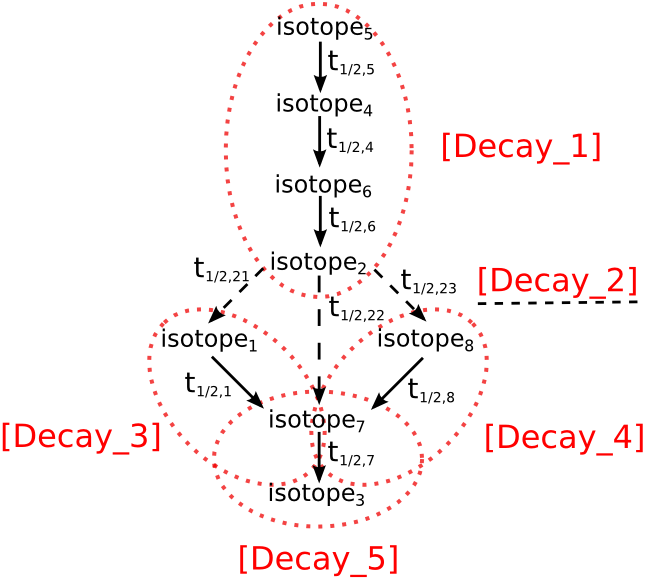
\includegraphics[width = 8cm]{\fig /decay_chain.png}
%  \caption{Decay chain with branches.}
%  \label{pic:dec_branches}
% \end{figure}
% 
% 
% When it comes to a simulation of first order reactions, the kinetic constant is given as an input. 
% The description of a kinetic chemical reaction has obviously two folowing forms
% \[
%   \begin{array}{l}
%     A\xrightarrow{k}B,\\
%     \frac{dc^A}{dt} = -k \cdot c^A.
%   \end{array}
% \]
% The first one description is a standard chemical one. The second equation describes temporal decrease in amount of concentrations of the specie $c^A$. The constant $k$ is so called kinetic constant and for the case of a first order reactions it is equal to so called reaction rate. The order of reaction with just one reactant is equal to the power of $c^A$ in partial diferential reaction.
% 
% For an inclusion of first order reaction into a reaction matrix a half-life needs to be computed from the corresponding kinetic constant $k$. The derivation follows
% \[
%   \begin{array}{l}
%     A\xrightarrow{k} B\\
%     \frac{dc^A}{d\tau} = -k\cdot c_A\\
%     \frac{dc^A}{c^A} = -k\cdot d\tau\\
%     \int\limits_{c^A_0/2}^{c^A_0}\frac{dc^A}{c^A} = -k\cdot\int\limits_{t_{1/2,A}}^{0} d\tau\\
%     \left[ ln c^A\right]_{c^A_0/2}^{c^A_0} = -[k\tau]_{t_{1/2,A}}^{0}\\
%     ln c^A_0 - \ln\frac{c^A_0}{2} = k\cdot t_{1/2,A}\\
% %     c^A (t) = c^A_0\cdot e^{-k\cdot t_{1/2,A}}\\
% %     {\bf substitution} \qquad c^A(t_{1/2,A}) = \frac{1}{2}\cdot c^A_0\\
% %     \frac{1}{2} c^A_0 = c^A_0\cdot e^{-k_1\cdot t_{1/2,A}}\\
%     \ln 2 = k \cdot t_{1/2,A}\\
%     t_{1/2,A} = \frac{ln 2}{k}
%   \end{array}                                                                                                                                                                                                                                                                                                            
% \]
% The matrix ${\bf R}$ is constructed in the same way as for the radioactive
% decay.

\subsection{General Chemical Reactions}
For a simulation of general chemical reactions as a part of reactive transport simulation, an application Semchem has been merged together with Flow123D. It enables to simulate following types of reactions:
\begin{itemize}
  \item Chemical equilibrium (solved using iterative Newtons method)
    \subitem mathematical description $K^{(r)} = \prod_i c_i^{\alpha_i^{(r)}},$

  \item Slow evolving chemical kinetics (solved using Runge-Kutta method)
    \subitem mathematical description $\frac{dc_i}{dt} = -k^{(r)}\prod_j c_j^{\beta_j^{(r)}},$

  \item Fast evolving chemical kinetics (discretized using implicit Eulerova method and solved using Newtons method)
     \subitem mathematical description $\frac{c_i^{(T+1)} - c_i^{T}}{\Delta t} = -k^{(r)}\prod_j c_j^{\beta_j^{(r),(T+1)}},$
  \item Radioactive decay can be simulated as a special case of first order reaction.
\end{itemize}

Further informations can be found in ``Snizeni poctu nelinearnich rovnic popisujicich chemicke reakce''.


\chapter{File formats}
%\section{Input format}


\chapter{New input files}
The input consists of the root input file given as the parameter on the command line and possibly several other 
files with large input data. In this section we shall describe format of the input files. At first, we specify syntax of
an extension to the JSON file format. Then we set rules for input of more specific data constructs. We continue by description of general scheme for input of
boundary conditions and material time-space variable data. And finally, we describe setting of particular equations and their solvers.

The aim of this draft is twofold. First, we want to outline the way how to translate current input file format (in version 1.6.5) into the new one without extending 
the existing functionality. Second, we want to propose a new way how to input general boundary and material data. Desired features are:
\begin{itemize}
 \item input simple data in simple way
 \item possibility to express very complex input data 
 \item possibility to generate data automatically, and input very large input sets
 \item input interface that provides uniform access to the data in program independent of the input format
\end{itemize}
[ ... something else?]

As this is a draft version there are lot of remarks, suggestions and questions in square brackets. Some keys are marked OBSOLETE, which means that 
we want to replace them by something else.

\section{Root file format}
The root input file is in the Humanized JSON file format. That is the JSON file format with few syntax extensions and several semantic rules particular to
Flow123d. The syntax extensions are
\begin{enumerate}
\item You can use one line comments using hash \verb'#'.
\item The quoting of the keys is optional if they do not contain spaces (holds for all Flow keys).
\item You can use equality sign \verb'=' instead of colon \verb':' for separation of keys and values in JSON objects.
\item You can use any whitespace to separate tokens in JSON object or JSON array.
\end{enumerate}
The aim of these extensions is to simplify writing input files manually. However these extensions can be easily filtered out and converted to 
the generic JSON format. (This way it can be also implemented in Flow123d.)

For those who are not familiar with the JSON file format, we give the brief description right here. The full description can be found at
\url{http://www.json.org/}. However, we use term {\it record} in the place of the {\it JSON object} in order to distinguish {\it JSON object}, 
which is merely a data structure written in the text, and the {\it C++ object}, i.e. instance of some class. 

\subsection{Humanized JSON}
The JSON format consists of four kind of basic entities: 
{\it null} token, {\it true} and {\it false} tokens, {\it number}, {\it string}. {\it Number} is either integer or float point number 
possibly in the exponential form and {\it string} is any sequence of characters quoted in \verb'""' (backslash \verb"\" is used as escape character and 
Unicode is supported, see full specification for details). 

In the following, we mean by white space characters:
space, tab, and new line. In particular the newline character (outside of comment or quoting) is just the white space character without any special meaning.

The basic entities can be combined in composed entities, in a {\it record} or in an {\it array}. The {\it record} is set of assignments enclosed in the curly brackets
\begin{verbatim}
{
        #basic syntax
        "some_number":124, 
        "some_string":"Hallo",
        "some_subrecord":{},
        "some_array":[],
        
        #extended syntax
        non_quoted_key_extension=123,
        separation_by_whitespace="a" sbw_1="b"
        sbw_2="c"
}
\end{verbatim}
One assignment is a pair of the {\it key} and the {\it value}. {\it Key} is {\it string} or token matching regexp\\
\verb'[a-zA-Z_][a-zA-Z_0-9]*'.
{\it Value} is basic or composed entity.
The key and the value are separated by the colon (generic syntax) or equality sign (extended syntax). Pairs are separated by a comma (generic syntax) or 
sequence of white space characters (extended syntax). The values stored in the record are accessed through the keys like in an associative array. Records are usually used for initialization of corresponding classes.

The second composed entity is the {\it array} which is sequence of (basic or composed) entities separated by comma (generic syntax) or whitespace sequence 
(extended syntax) and enclosed in the square brackets. 
The values stored in the array are accessed through the order. The Flow reader offers either initialization of a container from JSON array or
a sequential access. The latter one is the only possible access for the included arrays, which we discuss later.

On any place out of the quoted string you can use hash mark \verb'#' 
to start a one line comment. Everything up to the new line will be ignored and replaced by single white space.

[What about multiple line strings? (Should be allowed)]

\subsection{Special keys}
Apart from small extensions of JSON syntax, we impose further general rules on the interpretation of the input files by Flow123d reader.
First, the capital only keywords  
have a special meaning for Flow JSON reader. On the other hand, we use only small caps for keys interpreted through the reader.
The special keywords are:
\begin{description}

\item[TYPE]:\\ 
\begin{verbatim}
TYPE= <enum>
\end{verbatim}
The \verb'<enum>' is particular semantic construct described later on. 
When appears in the record, it specifies which particular class to instantiate. This only has meaning if the record initializes
an abstract class. In consistency with the source code, we shall call such records {\it polymorphic}. 


In fact we consider
that every record is of some {\it type} at least implicitly. The {\it type} of the record is specification of the keys that are
interpreted by the program Flow123d. At some places the program assumes a record of specific {\it type} so you need not to specify 
\verb'TYPE' key in those records.

\item[INCLUDE\_RECORD]:\\
This is a simple inclusion of another file as a content of a record:
\begin{verbatim}
{
        INCLUDE_RECORD = "<file name>"
}
\end{verbatim}

\item[INCLUDE\_ARRAY]:\\
\begin{verbatim}
array=
{
        INCLUDE_ARRAY = "<file name>"
        FORMAT = "<format string>"
}       
\end{verbatim}
The reader will substitute the include record by a sequentially accessible array. The file has fixed number of 
space separated data fields on every line. Every line becomes one element in the array of type record. Every line forms a 
record with key names given by the \verb'<format string>' 
and corresponding data taken form the line.

The key difference compared to regular JSON arrays is that included arrays can be accessed only sequentially 
within the program and thus we minimize reader memory overhead for large input data. The idea is to translate raw data into structured
format and use uniform access to the data.

Basic syntax for format string could be an array of strings --- formats of individual columns.
Every format string is an address of key that is given the column. Onother possibility is to give an arbitrary 
JSON file, where all values are numbers of columns where to take the value.

[\dots better specify format string]


[Possible extensions:
- have sections in the file for setting time dependent data
- have number of lines at the beginning
- have variable format
- allow vectors in the 'line records']

\item[REFERENCE]:\\
\begin{verbatim}
time_governor={
  REF=<address>
}
\end{verbatim}
This will set key \verb'time_governor' to the same value as the entity specified by the address.
The address is an array of strings for keys and integers for indices.
The address can be absolute or relative identification of an entity. The relative address is relative to the entity in which the reference record is contained.
One can use string \verb'".."' to move to parent entity and string \verb'"//"' to move to the root record of current file.
Indices in address starts from 0.

For example assume the file
\begin{verbatim}
mesh={
        file_name="xyz"
}
array=[
        {x=1, y=0}       
        {x=2, y=0}
        {x=3, y=0}
]               
outer_record={
        output_file="x_out"
        inner_record={
                output_file={REF=["..","output_file"]}  # value "x_out"
        }
        x={REF="/array/2/x"}                                    # value "3"
        f_name={REF=["//","mesh","file_name"]}                  # value "xyz"
}       
\end{verbatim}

Concept of addres should be better explained and used consistently in reader interface.
\end{description}

\subsection{Semantic rules}

\subsubsection{Implicit creation of composed entities}
Consider that there is a {\it type} of record in which all keys have default values (possibly except one). Then the specification
of the record {\it type} can contain a {\it default key}. Then user can use the value of the {\it default key} instead of the whole record.
All other keys apart from the {\it default key} will be initialized by default values. 
This allows to express simple tasks by simple inputs but still make complex inputs possible. 
In order to make this working, developers should provide default values everywhere it is possible.
 
Similar functionality holds for arrays. If the user sets a non-array value where an array is expected the reader provides an array with a unique element holding the given value.
See examples in the next section for application of these two rules.



\subsubsection{Enum construct}
Enum values can be integers or strings from particular set. Strings should be preferred for manual creating of input files, while 
the integer constants are suitable for automatic data preparation. 

The input reader provides a way how to define names of members of an enum class and then 
initialize this enum class from input file.  [Need better description]

\subsubsection{String types}
For purpose of this documentation we distinguish several string types with particular purpose and treatment. Those are:
\begin{description}
\item[input filename] This has to be valid absolute or relative path to an existing file. 
The string can contain variable \verb'${INPUT}' %$
which will be replaced by path given at command line through parameter \verb'-i'.

[In order to allow input of  time dependent data in individual files, we should 
 have also variable \verb'${TIME\_LEVEL}' %$
 From user point of view this is not property of general input filename string, however
 in implementation this should be done in the same way as \verb'${INPUT}'.
]
 
[? Shall we allow both Windows and UNIX slashes?]

[Developers should provide default names to all files. ]

\item[output filename] This has to be relative path. The path will be prefixed by
the path given at command line through the parameter \verb'-o'.
In some cases the path will be also postfixed by extension of particular file format.

\item[formula] Expression that will be parsed and evaluated runtime. Documentation of particular key should provide 
variables which can appear in the expression, however in general it can be function of the space coordinates $x$, $y$, $z$ and possibly also 
function of time $t$. For full specification of expression syntax see documentation of FParser library:
\url{http://warp.povusers.org/FunctionParser/fparser.html\#literals}

\item[text string] Just text without particular meaning.
\end{description}

\subsubsection{Record types}
A record type like particular definition of a class (e.g. in C++). One record type serves usually for initialization of 
one particular class. From this point of view one record type is set of keys that corresponding class can read.

For purpose of this manual the record type is given by specification of record's keys, their types, default values and meanings.
In the next two sections, we describe all record types that forms input capabilities of Flow123d. Description of a record type 
has form of table. Table heading consists of the name of the record type. Then for every key we present name, type of the value,
default value and text description of key meaning. Type of the value can be record type, array of record types, double, integer, enum or 
string type. Default value specification can be:
\begin{description} 
 \item[none] No default value given, but input is mandatory. You get an error if you don't set this key.
 \item[null] \verb'null' value. No particular default value, but you need not to set the key. Usually means feature turned off.
 \item[explicit value] For keys of type: string, double, integer, or enum, the default value is explicit value of this type.
 \item[type defaults] For keys of some record type we let that record to set its default values.
\end{description}

[? polymorphic record types]


\section{Record types for input of data fields}


\newenvironment{recordtype}[2]
{\par
 \vskip 2ex
 \noindent%
 record type: {\bf #1}#2
 \par%
 \vskip 0.5ex
 \hrule%
 \vskip 0.3ex
 \hrule
 \begingroup%records of steady field type which we describe right now 
  \addtolength{\leftskip}{3em}%
  %
  \gdef\keyitem##1##2##3{%
    \par
    \vskip 0.3ex
    %\hrule%
    \noindent%
    \hspace{-3em}{\bf\tt ##1} = {\it \textless ##2\textgreater} \hfill \makebox[0.4\textwidth][l]{DEFAULT: {##3}\hfil}%
    \par
  }%
}{%
  \vskip 0.7ex  
  \hrule%
  \vskip 0.5ex
  \endgroup%
}

\def\enumhead#1{
{\bf #1} enum cases:
}
\def\enumitem#1#2{
  \par{\tt #1=#2 \hspace{2em}}
}

In this section we describe record types used to describe general time-space scalar, vector, or tensor fields
and records for prescription of boundary conditions. Since one possibility how to prescribe input data fields is by 
discrete function spaces on computational mesh, we begin with mesh setting.

\subsection{Mesh type}
The mesh record and should provide a mesh consisting of points, lines, triangles and tetrahedrons in 3D space and further
definition of boundary segments and element connectivity.

\begin{recordtype}{Mesh}{}

\keyitem{file}{input filename}{mesh.msh}
The file with computational mesh in the ASCII GMSH format.\\
\url{http://geuz.org/gmsh/doc/texinfo/gmsh.html#MSH-ASCII-file-format}

\keyitem{boundary\_segments}{array of boundary segments}{null optional}
The set of 0,1, or 2 dimensional boundary faces of the mesh should be partitioned into boundary segments in order to prescribe unique boundary condition 
on every boundary face. 
The segments numbers are assigned to boundary faces by iterating through the array. Initially every boundary face has segment number $0$. 
Every record in the array use ``auxiliary'' physical domains, elements or direct face specification to specify some set of boundary faces. The new segment number
is assigned to each face in the set, possibly overwriting previous value.

Physical domains or its parts that appears in the boundary segment definitions are removed form the computational mesh, however, the element
numbers of removed elements are stored in the corresponding boundary face and can be used to define face-wise approximations of functions with 
support on the boundary.

\keyitem{neighbouring}{input file name}{neigbours.flw}
This should be removed as soon as we integrate ngh functionality into flow.
\end{recordtype}

\begin{recordtype}{Boundary segment}{}
 \keyitem{index}{integer}{index in outer array}
 The index of boundary segment can be used later to prescribe particular type of boundary condition on it.
 Indices must be greater or equal to $1$ and should form more or less continuous sequence. The zero boundary segment is reserved for remaining part
 of the boundary. By default we assign indices to boundary segments according to the order in their array in mesh, i.e. index (counted form $0$) plus $1$.
 \keyitem{physical\_domains}{array of integers}{null optional}
 Numbers of physical domains which form the boundary segment. All elements of these physical domains will be removed from actual computational mesh.
 \keyitem{elements}{array of integers}{null optional}
 The array contains element numbers which should be removed from computational mesh and added to boundary segment.
 \keyitem{sides}{array of integer pairs}{null optional}
 The array contains numbers of elements which outer faces will be added to the boundary segment or pairs $[element, side\_on\   _element]$ 
 identifying individual faces that will be added to the boundary segment.
\end{recordtype}

\subsection{Time-space field type}
A general time and space dependent, scalar, vector, or  tensor valued function is given by array
of {\it steady field data}, i.e. time slices. The time slice contains array of {\it space functions}
for individual materials. Then, the {\it space function} can by either analytical (given by formula)
or numerical, given by type of discrete space and array of {\it elemental functions}. {\it Elemental function} is
just array of values for every degree of freedom on one element.

The function described by this type is tensor values in general and dimensions of this tensor should be 
specified outside of the function data. For example in description of Transport record type you should specify that function
for initial condition is vector valued with vector size equal to number of substances. It is like template for Time-space field
type parametrized by shape of the value tensor given by number of lines $N$ and columnes $N$.


\begin{recordtype}{Steady field data}{}
\keyitem{time}{double}{-Inf}
  Start time for the spatial filed data. 
\keyitem{time\_interpolation}{enum}{constant}
  \enumhead{time interpolation}
  \enumitem{constant}{0} Keeps constant data until next time cut.
  \enumitem{linear}{1} Linear interpolation between current time cut and the next one.
\keyitem{materials}{array of Steady spatial functions}{null optional}
\end{recordtype}

\begin{recordtype}{Space function}{}
\keyitem{material}{integer}{0}
Material filter. The function has nonzero value only on elements with given material number. 
Function with filter $0$ takes place for all materials where no function is set.

\keyitem{analytic}{multi-array of function formulas}{null optional}
The shape of the multi-array is given by 
rank of the value of the function. Since formula parser can deal only with scalar functions, we
have to specify individual members of resulting tensor. Formulas can contain variables $x$, $y$, $z$, and $t$. 
The formula is used until the next time slice and is evaluated for every solved time step (can depend on equation).

Instead of constant formulas one can use double values.
Usage of formulas or doubles need not to be uniform over the tensor.


\keyitem{numeric\_type}{enum}{None}
  \enumhead{FE space}
  \enumitem{None}{0} Use analytic function.
  \enumitem{P0}{1} Zero order polynomial on element.

Currently we support only P0 base functions for data.

\keyitem{numeric}{array of element functions}{empty array}
Usually, this element-wise array should by included from an external file through \verb'INCLUDE_ARRAY' construct.

\end{recordtype}

\begin{recordtype}{Element function}{}
\keyitem{element\_id}{integer}{null optional}
Element ID in the mesh. By default the element is 
identified by the index in the array of element function.

\keyitem{values}{multi-array of doubles}{null mandatory}
Values for degrees of freedom of the base functions on the element. Currently we support 
only P0 functions which are given by value in the barycenter of the element. 
In general the value can be tensor, i.e. array of arrays of doubles.
However, in accordance to simplification rules, you can use only array of doubles for 
vector functions or mere double for scalar functions.
\end{recordtype}

[ tensor/vector valued element function should be given also as simple array of DOF values. But
  we have to provide ordering of tensor products of FE spaces]

[ As follows from next examples, there is no way how to simply set simply tensors.  We can introduce automatic conversion form scalar to  vector (constant vector) and vector to tensor 
(diagonal tensor). ]

[ we should also allow 'in place' array includes to simplify material tables etc.]

[How to allow parallel input of field data?]

[Should be there explicit mesh reference in the field specification?]


Examples:
\begin{verbatim}
constant_scalar_function = 1.0
# is same as
constant_scalar_function = {
  time = -Inf,
  time_interpolation= constant,
  materials = [
    {
      rank=0
      numeric_type=None
      analytic=1.0       # the only key withou default value
    }
  ]
}

conductivity_tensor = 
  [{ material = 1,
     rank = 2,
     analytic = [[1.0, 0.0, 0.0], [0.0, 1.0, 0.0], [0.0, 0.0, 1.0]]
   },
   { material = 2,
     rank = 2,
     analytic = [[10.0, 0.0, 0.0], [0.0, 10.0, 0.0], [0.0, 0.0, 10.0]]
   }
  ]
 
\end{verbatim}

\subsection{Boundary conditions}
Input of boundary conditions is similar to the Time-space fields. For description of one time slice we have 
type {\it steady boundary data}. This contains array of {\it boundary conditions} for individual boundary segments. 
{\it Boundary condition} is given by type and parameters that are analytic or numeric functions. However, numeric functions
are considered only on boundary elements.

\begin{recordtype}{steady boundary data}{}
\keyitem{time}{double}{0.0}
Time when the BC should be applied.
\keyitem{bc}{array of boundary conditions}{empty} 
\end{recordtype}

\begin{recordtype}{boundary condition}{}
 \keyitem{boundary\_segment}{integer}{0}
  Boundary segment where the boundary condition will be applied.
 \keyitem{bc\_type}{enum}{dirichlet}
  Currently there are just three types of boundary condition common to all equations, 
  but some equations can implement some specific boundary conditions. Common boundary condition  types are
  \enumhead{BC types}
  \enumitem{dirichlet}{0}
  \enumitem{neumann}{1}
  \enumitem{newton}{2} (also known as Robin boundary condition)


\keyitem{value}{space function}{type defaults}
Prescribed value for Dirichlet boundary condition and Newton boundary condition, the normal flux for the Neumann boundary condition.
Key \verb'material' of {\it space function} is irrelevant.

\keyitem{mean\_value}{scalar or vector constant}{0}
Prescribes flux for Neumann boundary condition by total flux over the boundary segment. If both {\it value} and {\it mean\_value} keys
are set, we use only {\it value} key. 
[How this interact with fracture opening?]


\keyitem{newton\_coef}{scalar space function}{type defaults}
Coefficient that appears in the Newton boundary condition. Key \verb'material' of {\it space function} is irrelevant.
\end{recordtype}

E.g. denoting $u$ the unknown scalar or vector field and $\prtl_n u$ density of the normal flux of this field,
the meaning of keys \verb'value' and \verb'newton_coef' is following:
$\vc{v}$ $\grad v$
\begin{align*}
 u &:= value &&\text{for Dirichlet boundary} \\
 A\grad u \cdot \vc{n} &:= value && \text{for Neumann  boundary} \\
A\grad u \cdot \vc{n} &:= newton_coef ( u - value ) && \text{for Newton boundary}
\end{align*}

Specific interpretation of the boundary conditions should be described in particular equations.

[How to allow both analytic  and numerical functions here?]

[ In order to allow changing BC type in time, the structure has to be: time array of BC segments array of BC type with data
alternatively we can have just one array of BC patches, where one patch has: time, BC segment, BC type, BC data
patches with non monotone time will be scratched]

[need vector valued Dirichlet (and Neuman, and Newton) for Transport boundary conditions]

[More examples...]


\section{Other record types recognized by Flow123d}

\subsection{Record types not related to equations}

\begin{recordtype}{Root record}{}
  \keyitem{system}{system type}{type defaults}
  Record with application setting.
  \keyitem{problem}{problem type}{null mandatory}
  Record with numerical problem to solve. 
  \keyitem{material}{input filename}{material.flw}
    Old material file still used for initialization of data fields in equations. 
    This should be replaced by material database type. Then certain input data fields in equations can be 
    constructed from material informations. Main obstacle are various adsorption algorithms depending on material number.
\end{recordtype}

Only these  keys are recognized directly at main level, however you can put here your own keys and then reference
to them. For example \verb'mesh' is part of problem type record, but you can put it on the main level and use reference 
inside \verb'problem'. 

[Should we put problem record to the main level?]

[Should we provide ``material database''? Possibility to specify properties of individual materials and use them to construct
 field data for equations.]

\begin{recordtype}{System}{}
\keyitem{pause\_after\_run}{bool}{no}
Wait for press of Enter after run. Good for Windows users, but dangerous for batch computations. 
Should be rather an command-line option.
\keyitem{verbosity}{bool}{no}
Turns on/off more verbose mode. 
\keyitem{output\_streams}{output stream}{null optional}
One or more output data streams.
There are two predefined output streams:


vtk ascii stream:
\begin{verbatim}
{
  name="dafault_vtk_ascii"
  file="flow_output"
  type="vtk_ascii"
}
\end{verbatim}

GMSH ascii stream:
\begin{verbatim}
{
  name="dafault_gmsh_ascii"
  file="flow_output"
  type="gmsh_ascii"
}
\end{verbatim}

\end{recordtype}

Possibly here could be variables for check-pointing, debugging, timers etc.

\begin{recordtype}{Output stream}{}
 \keyitem{name}{string}{null mandatory}
  Name of the output stream. This is used to set output stream for 
  individual output data. 
 \keyitem{file}{output filename string}{stream name}
  File name of the output file for the stream. The file name should be without extension, the correct extension
  will be appended according to the format type.
 \keyitem{format}{enum}{vtk\_ascii}
   \enumhead{output format}
   \enumitem{vtk\_ascii}{0} 
   \enumitem{gmsh\_ascii}{1}
 \keyitem{precision}{integer}{8}
 Number of valid decadic digits to output floating point data into the ascii file formats.
 \keyitem{copy\_file}{output filename string}{null optional}
 Optionally one can set copy file to output data into to different file formats.
 \keyitem{copy\_format}{enum}{null optional}
 \keyitem{copy\_precision}{integer}{8}
\end{recordtype}


\subsection{Equation related record types}
Up to now there is only one problem type: \verb'TYPE=sequential\_coupling', 
but in near future we should introduce full coupling e.g. for density driven flow.

The {\emph sequential coupling problem} has following keys:
\begin{recordtype}{Sequential coupling}{ implements {\it Problem type} }
\keyitem{description}{string}{null optional}
Short text description of solved problem. Now it is only reported on the screen, but could be 
written into output files or used somewhere else.
%
\keyitem{mesh}{mesh type}{type defaults}
The computational mesh common for both coupled equations.
%
\keyitem{time\_governor}{time governor type}{type defaults}
Common time governor  setting.
[ Future: allow different setting for each equation]
%
\keyitem{primary\_equation}{darcy flow type}{type defaults}
Independent equation.
%
\keyitem{secondary\_equation}{transport type}{null optional}
Equation with some data dependent on the primary equation.
\end{recordtype}

\begin{recordtype}{Time governor}{}
\keyitem{init\_time}{double}{0.0}
Time when an equation starts its simulation.
\keyitem{time\_step}{double}{1.0}
Initial time step.
\keyitem{end\_time}{double}{1.0}
End time for an equation. 
\end{recordtype}

This record type should initialize \verb'TimeGovernor' class, but there are still questions about steady TimeGovernor and 
if we allow user setting for other parameters.

There are three subtypes {\it steady saturated MH}, {\it unsteady saturated MH}, {\it unsteady saturated LMH}
The common keys are:

\begin{recordtype}{Darcy flow}{(abstract type)}
\keyitem{TYPE}{enum}{}
  There are three implementations of Darcy flow. Most keys are common but unsteady solvers accept some extra keys.
  \enumhead{darcy flow type}
  \enumitem{steady\_MH}{0}
  \enumitem{unsteady\_LMH}{1}
  \enumitem{unsteady\_MH}{2}
\keyitem{sources}{time-space field}{0} Density of water sources. Scalar valued field (1x1 tensor).
\keyitem{sources\_file}{input file name}{null optional}
File with sources in old format. (OBSOLETE)
%
\keyitem{coef\_tensor}{tensor steady field}{1.0}
Conductivity 3x3 tensor. [Should be always 3x3 and then restricted on 2d and 1d fractures.]
\keyitem{boundary\_condition}{array of steady boundary data}{null mandatory} 
New scheme for setting boundary conditions.
\keyitem{boundary\_file}{input file name}{null mandatory}
File with boundary conditions in old format. (OBSOLETE)
%
\keyitem{solver}{solver type}{type defaults}
\keyitem{n\_schurs}{integer}{2}
Number of Schur complements to make. Valid values are 0,1,2.
%
\keyitem{output}{darcy flow output type}{typ defaults}
This is just sub record to separate output setting. 
%
\keyitem{initial}{steady data type}{null mandatory}
Initial condition. Scalar valued field (1x1 tensor). (for unsteady only)
\keyitem{initial\_file}{input file name}{null mandatory}
File with initial condition in old format. (OBSOLETE)
%
\keyitem{storativity}{steady data type}{null mandatory}   
Storativity coefficient. Scalar valued field (1x1 tensor). (for unsteady only)
\end{recordtype}

\begin{recordtype}{Darcy flow output}{}
\keyitem{save\_step}{double}{null optional}
Time step between outputs.
\keyitem{output\_times}{array of doubles}{null optional}
Force output in prescribed times. Can be combined with regular otuptu given by \verb'save_step'.
\keyitem{velocity\_p0}{output stream name}{default\_vtk\_ascii}
\keyitem{pressure\_p0}{output stream name}{default\_vtk\_ascii}
\keyitem{pressure\_p1}{output stream name}{default\_vtk\_ascii} 
\end{recordtype}
 


\subsection{Solver type}
\begin{recordtype}{Solver type}{ (abstract)}
 \keyitem{TYPE}{enum}{petsc}
 \enumhead{solver types}
 \enumitem{petsc}{0} Use any PETSc solver for MPIAIJ matrices.
 \enumitem{bddc}{1} Use BDDC solver (need not to work with every equation).
 %
 \keyitem{accuracy}{double}{solvers defaults}
 Absolute residual tolerance. 
 \keyitem{max\_it}{integer}{1000}
 Maximum number of outer iterations.
 \keyitem{parameters}{string}{null optional}
 String with options for PETSc solvers.
 \keyitem{export\_to\_matlab}{bool}{no}
 Save every solved system in matlab format. Useful for debugging and numerical experiments.
 %
\end{recordtype}


\subsection{Transport type}
\begin{recordtype}{Transport type}{}
 \keyitem{sorption}{bool}{no}
 \keyitem{dual\_porosity}{bool}{no}
 \keyitem{transport\_reactions}{bool}{no}
 What kind of reactions is this? Age of water?
 %
 \keyitem{reactions}{reaction type}{null optional}
 Currently only Semchem is supported. [Interface to Phreaq ...]
 \keyitem{decays}{array of decays}{null optional}
 \keyitem{substances}{array of strings}{null mandatory}
 Names for transported substances. Number of substances is given implicitly by size of the array.
 %
 \keyitem{initial}{steady data type}{null mandatory}
 Vector valued initial condition for mobile phase of all species. 
 \keyitem{initial\_others}{steady data type}{null optional}
 Tensor valued initial condition for immobile, mobile-sorbed, immobile-sorbed phases and all species. (3 x n\_substances).
 [alternatively have separate key for each phase]
 \keyitem{initial\_file}{input file name}{null mandatory}
 File with initial condition in old format. (OBSOLETE)
 %
 \keyitem{boundary\_condition}{array of steady boundary data}{null mandatory} 
 New scheme for setting boundary conditions.
 \keyitem{boundary\_file}{input file name}{null mandatory}
 File with boundary condition in old format. (OBSOLETE)
 For time dependent boundary conditions, the filename is postfixed with 
 number of time level.
 \keyitem{bc\_times}{array of doubles}{null optional}
  Times for changing boundary conditions. If you set this variable, you have to prepare a separate file with boundary conditions for every 
  time in the list. Filenames for individual time level are formed from BC filename by appending underscore and three digits of time level number, e.g. 
  {\tt transport\_bcd\_000, transport\_bcd\_001, etc.} (OBSOLETE)
 \keyitem{output}{transport output}{type defaults}  

\end{recordtype}

\begin{recordtype}{Transport output}{}
\keyitem{save\_step}{double}{null optional}
Time step between outputs.
\keyitem{output\_times}{array of doubles}{null optional}
Force output in prescribed times. Can be combined with regular otuptu given by \verb'save_step'.
\keyitem{mobile\_p0}{output stream name}{default\_vtk\_ascii}
\keyitem{immobile\_p0}{output stream name}{default\_vtk\_ascii}
\keyitem{mobile\_sorbed\_p0}{output stream name}{default\_vtk\_ascii} 
\keyitem{immobile\_sorbed\_p0}{output stream name}{default\_vtk\_ascii} 
\keyitem{mobile\_p1}{output stream name}{default\_vtk\_ascii}
\keyitem{immobile\_p1}{output stream name}{default\_vtk\_ascii}
\keyitem{mobile\_sorbed\_p1}{output stream name}{default\_vtk\_ascii} 
\keyitem{immobile\_sorbed\_p1}{output stream name}{default\_vtk\_ascii} 
\end{recordtype}

\begin{recordtype}{Reaction}{}
% \key{Output\_precission} & \type{int} & 1 &
%Number of decimal places written to output file created by Semchem\_module.
%\\
%\hline
%\key{Number\_of\_further\_species} & \type{int} & 0 &
%Concentrations of these species are not computed, because they are ment to be unexghaustible.
%\\
%\hline
%\key{Temperature} & \type{double} & 0.0 &
%Temperature, one of state variables of the system.
%\\
%\hline
%\key{Temperature\_Gf} & \type{double} & 0.0 &
%Temperature at which Free Gibbs Energy is specified.
%\\
%\hline
%\key{Param\_Afi} & \type{double} & 0.0 &
%Parameter of the Debuy-H\"{u}ckel equation for activity coeficients computation.
%\\
%\hline
%\key{Param\_b} & \type{double} & 0.0 &
%Parameter of the Debuy-H\"{u}ckel equation for activity coeficients computation.
%\\
%\hline
%\key{Epsilon} & \type{double} & 0.0 &
%Epsilon specifies relative norm of residuum estimate to stop numerical algorithms used by Semchem\_module.
%\\
%\hline
%\key{Time\_steps} & \type{int} & 1 &
%Number of transport step subdivisions for Semchem\_module.
%\\
%\hline
%\key{Slow\_kinetics\_substeps} & \type{int} & 0 &
%Number of substeps performed by Runge-Kutta method used for slow kinetics simulation.
%\\
%\hline\\
%\key{Error\_norm\_type} & \type{string} & "Absolute" &
%Through wich kind of norm the error is measured.
%\\
%\hline\\
%\key{Scalling} & \type{boolean} & "No" &
%Type of the problem preconditioning for better convergence of numerical method.
%\\
%\hline\\
%\end{initable}
%\newpage
%\begin{initable}{Aqueous\_species}
%\key{El\_charge} & \type{int} & 0 &
%Electric charge of an Aqueous\_specie particleunder consideration.
%\\
%\hline
%\key{dGf} & \type{double} & 0.0 &
%Free Gibbs Energy valid for TemperatureGf.
%\\
%\hline
%\key{dHf} & \type{double} & 0.0 &
%Enthalpy
%\\
%\hline
%\key{Molar\_mass} & \type{double} & 0.0 &
%Molar mass of Aqueous\_species.
%\\
%\hline
%\end{initable}
%
%\begin{initable}{Further\_species}
%\key{Specie\_name} & \type{string} & "" &
%Name belonging to Further\_specie under consideration.
%\\
%\hline
%\key{dGf} & \type{double} & 0.0 &
%Free Gibbs Energy valid for TemperatureGf.
%\\
%\hline
%\key{dHf} & \type{double} & 0.0 &
%Enthalpy
%\\
%\hline
%\key{Molar\_mass} & \type{double} & 0.0 &
%Molar mass of Further\_species.
%\\
%\hline
%\key{Activity} & \type{double} & 0.0 &
%Activity of Further\_species.
%\\
%\hline
%\end{initable}
%
%\begin{initable}{Reaction\_i}
%\key{Reaction\_type} & \type{string} & "unknown" &
%Type of considered reaction (Equilibrium, Kinetics, Slow\_kinetics).
%\\
%\hline
%\key{Stoichiometry} & \type{int} & 0 &
%Stoichiometric coeficients of species taking part in $i$-th reaction.
%\\
%\hline
%\key{Kinetic\_constant} & \type{double} & 0.0 &
%Kinetic constant for determination of reaction rate.
%\\
%\hline
%\key{Order\_of\_reaction} & \type{int} & 0 &
%Order of kinetic reaction for participating species.
%\\
%\hline
%\key{Equilibrium\_constant} & \type{double} & 0.0 &
%Equilibrium constant defining i-th reaction.
%
\end{recordtype}

\begin{recordtype}{Decay chain}{}
\keyitem{substance\_ids}{array of integers}{empty}
Sequence of $N$ ids of transported substances describing the order of isotopes in the decay chain.
\keyitem{half\_lives}{array of doubles}{empty}
This array of $N-1$ half-lives of individual decays.
If there are no bifurcation key specified, the decay chain is linear $1\to 2 \to 3$.
If there is the bifurcation key, the decay chain is branched $1\to 2, 1\to 3$.
\keyitem{bifurcation}{array of double}{null optional}
Contains $N-1$ probabilities for individual branches of the bifurcation decay.
They should sum to one.
\end{recordtype}




\section{Other input files}
% Copyright (C) 2007 Technical University of Liberec.  All rights reserved.
%
% Please make a following refer to Flow123d on your project site if you use the program for any purpose,
% especially for academic research:
% Flow123d, Research Centre: Advanced Remedial Technologies, Technical University of Liberec, Czech Republic
%
% This program is free software; you can redistribute it and/or modify it under the terms
% of the GNU General Public License version 3 as published by the Free Software Foundation.
%
% This program is distributed in the hope that it will be useful, but WITHOUT ANY WARRANTY;
% without even the implied warranty of MERCHANTABILITY or FITNESS FOR A PARTICULAR PURPOSE.
% See the GNU General Public License for more details.
%
% You should have received a copy of the GNU General Public License along with this program; if not,
% write to the Free Software Foundation, Inc., 59 Temple Place - Suite 330, Boston, MA 021110-1307, USA.


\subsection{Mesh file format version 2.0}
\label{mesh_file}

The only supported format for the computational mesh is MSH ASCII format produced 
by the GMSH software. You can find its documentation on:

\url{http://geuz.org/gmsh/doc/texinfo/gmsh.html#MSH-ASCII-file-format}

Comments concerning Flow123d:
\begin{itemize}
  \item Every inconsistency of the file stops the calculation.
    These are:
      \begin{itemize}
        \item Existence of nodes with the same \vari{node-number}.
        \item Existence of elements with the same \vari{elm-number}.
        \item Reference to non-existing node.
        \item Reference to non-existing material (see below).
        \item Difference between \vari{number-of-nodes} and actual number of
          lines in nodes' section.
        \item Difference between \vari{number-of-elements} and actual number of
          lines in elements' section.
      \end{itemize}
  \item By default Flow123d assumes meshes with \vari{number-of-tags} = 3. 
    \begin{description}
    \item[\vari{tag1}] is number of material (reference to {\tt
    .MTR} file) in the element.
    \item[\vari{tag2}] is number of geometry region in which the element lies. 
    \item[\vari{tag3}] is partition number (CURRENTLY NOT USED).
    \end{description}
    In accordance with specification of GMSH mesh format.
  \item Currently, line (\vari{type} = 1), triangle (\vari{type} = 2) and
    tetrahedron (\vari{type} = 4) are the only supported types
    of elements. Existence of an element of different type stops the calculation.
  \item Wherever possible, we use the file extension {\tt .MSH}. It is not
    required, but highly recomended.
  \item This file format can be used also for storing simple dicrete scalar or vector fields. We support output
   into this format (see Section \ref{section_output})
\end{itemize}

%%%%%%%%%%%%%%%%%%%%%%%%%%%%%%%%%%%%%%%%%%%%%%%%%%%%%%%%%%%%%%%%%%%%%%%%%%%%%%%%%%%%%%%%%%%%%
\subsection{Neighbouring file format, version 1.0}
\label{ngh_file}

The file is divided in two sections, header and data.
The extension {\tt .NGH} is highly recomended for files of this type.
\begin{fileformat}
\$NeighbourFormat\\
  1.0 \vari{file-type} \vari{data-size}\\
\$EndNeighbourFormat\\
\$Neighbours\\
  \vari{number-of-neighbours}\\
  \vari{neighbour-number} \vari{type} \vari{$<$type-specific-data$>$}\\
  \dots\\
\$EndNeighbours\\
\end{fileformat}
where
\begin{description}
 \ditem{file-type}{int} --- is equal 0 for the ASCII file format.
 \ditem{data-size}{int} --- the size of the floating point numbers used in
  the file. Usually \vari{data-size} = sizeof(double).
 \ditem{number-of-neighbours}{int} --- Number of neighbouring defined in the
  file.
 \ditem{neighbour-number}{int} --- is the number (index) of the n-th
  neighbouring. These numbers do not have to be given in a consecutive (or even an
  ordered) way. Each number has to be given only onece, multiple definition
  are treated as inconsistency of the file and cause stopping the
  calculation.
 \ditem{type}{int} --- is type of the neighbouring. 
 \ditem{$<$type-specific-data$>$}{} --- format of this list depends on the
  \vari{type}.
\end{description}
\subsection*{Types of neighbouring and their specific data}
    \begin{description}
      \ditem{type =}{10} --- ``Edge with common nodes'', i.e. sides of
        elements with common nodes. (Possible many elements)
      \ditem{type =}{11} --- ``Edge with specified sides'', i.e. sides of
        the edge are explicitly defined. (Possible many elements)
      \ditem{type =}{20} --- ``Compatible'', i.e. volume of an element with a
        side of another element. (Only two elements)
      \ditem{type =}{30} --- ``Non-compatible'' i.e. volume od an element with
        volume of another element. (Only two elements)
   \end{description}
   \begin{tabular}{|c|l|l|}
      \hline
      \vari{type} & \vari{type-specific-data} & Description \\
      \hline
      \hline
      10 & \vari{n\_elm} \vari{eid1} \vari{eid2} \dots & number of elements
      and their ids \\
      \hline
      11 & \vari{n\_sid} \vari{eid1} \vari{sid1} \vari{eid2} \vari{sid2} \dots
      & number of sides, their elements and local ids \\
      \hline
      20 & \vari{eid1} \vari{eid2} \vari{sid2} \vari{coef} & Elm 1 has to have
      lower dimension\\
      \hline 
      30 & \vari{eid1} \vari{eid2} \vari{coef} & Elm 1 has to have
      lower dimension\\
      \hline
   \end{tabular}

   \vari{coef} is of the {\tt double} type, other variables are {\tt int}s.
\subsection*{Comments concerning {\tt Flow123d}:}
\begin{itemize}
  \item Every inconsistency or error in the {\tt .NGH} file causes stopping
    the calculation. These are especially:
    \begin{itemize}
      \item Multiple usage of the same \vari{neighbour-number}.
      \item Difference between \vari{number-of-neighbours} and actual number
        of data lines.
      \item Reference to nonexisting element.
      \item Nonsence number of side.
    \end{itemize}
  \item The variables \vari{sid?} must be nonegative and lower than the number
    of sides of the particular element. 
\end{itemize}


%%%%%%%%%%%%%%%%%%%%%%%%%%%%%%%%%%%%%%%%%%%%%%%%%%%%%%%%%%%%%%%%%%%%%%%%%%%%%%
\subsection{Material properties file format, version 1.0}
\label{material_file}

The file is divided in two sections, header and data.
The extension {\tt .MTR} is highly recomended for files of this type.
\begin{fileformat}
\$MaterialFormat\\
  1.0 \vari{file-type} \vari{data-size}\\
\$EndMaterialFormat\\
\$Materials\\
  \vari{number-of-materials}\\
  \vari{material-number} \vari{material-type} \vari{$<$material-type-specific-data$>$}
  \vari{[text]}\\
  \dots\\
\$EndMaterials \\
\$Storativity \\
  \vari{material-number} \vari{$<$storativity-coefficient$>$}
  \vari{[text]}\\
  \dots\\
\$EndStorativity \\
\$Geometry\\
  \vari{material-number} \vari{geometry-type} \vari{$<$geometry-type-specific-coefficient$>$}
  \vari{[text]}\\
  \dots\\
\$EndGeometry \\
\$Sorption\\
  \vari{material-number} \vari{substance-id} \vari{sorption-type} \vari{$<$sorption-type-specific-data$>$}
  \vari{[text]}\\
  \dots\\
\$EndSorption \\
\$SorptionFraction\\
  \vari{material-number} \vari{$<$sorption-fraction-coefficient$>$}
  \vari{[text]}\\
  \dots\\
\$EndSorptionFraction \\
\$DualPorosity\\
  \vari{material-number} \vari{$<$mobile-porosity-coefficient$>$} \vari{$<$immobile-porosity-coefficient$>$}
  \vari{$<$nonequillibrium-coefficient-substance(0)$>$} \dots \vari{$<$nonequilibrium-coefficient-substance(n-1)$>$} 
  \vari{[text]}\\
  \dots\\
\$EndDualPorosity \\

\$Reactions\\
  \vari{reaction-type} \vari{$<$reaction-type-specific-coefficient$>$} 
  \vari{[text]}\\
  \dots\\
\$EndReactions \\

\end{fileformat}
where:
\begin{description}
 \ditem{file-type}{int} --- is equal 0 for the ASCII file format.
 \ditem{data-size}{int} --- the size of the floating point numbers used in
  the file. Usually \vari{data-size} = sizeof(double).
 \ditem{number-of-materials}{int} --- Number of materials defined in the
  file.
 \ditem{material-number}{int} --- is the number (index) of the n-th
  material. These numbers do not have to be given in a consecutive (or even an
  ordered) way. Each number has to be given only onece, multiple definition
  are treated as inconsistency of the file and cause stopping the
  calculation (exception \$Sorption section).
 \ditem{material-type}{int} --- is type of the material, see table.
 \ditem{$<$material-type-specific-data $>$}{} --- format of this list depends on the
  \vari{material~-~type}.
 \ditem{$<$storativity-coefficient$>$}{double} --- coefficient of storativity  
 \ditem{geometry-type}{int} --- type of complement dimension parameter (only for 1D and 2D material), 
 for 1D element is supported type 1 - cross-section area, for 2D element is supported type 2
 - thickness.  
 \ditem{$<$geometry-type-specific-coefficient$>$}{double} --- cross-section for 1D
 element or thickness for 2D element. 
 
 \ditem{substance-id}{int} --- refers to number of transported substance, numbering starts on \vari{0}.
 \ditem{sorption-type}{int} --- type 1 - linear sorption isotherm,
                             type 2 - Freundlich sorption isotherm,
                             type 3 - Langmuir sorption isotherm.
 \ditem{$<$sorption-type-specific-data $>$}{} --- format of this list depends on the
  \vari{sorption~-~type}, see table. 
  
 Note: Section \$Sorption is needed for calculation only if \vari{Sorption} is
   turned on in the \vari{ini} file.
 
 \ditem{$<$sorption-fraction-coefficient$>$}{double} --- ratio of the "mobile" solid surface in the contact with "mobile" water to the total solid
 surface (this parameter (section) is needed for calculation only if \vari{Dual\_porosity} and \vari{Sorption} is 
 together turned on in the ini file).                        
  
 \ditem{$<$mobile-porosity-coefficient$>$}{double} --- ratio of the mobile pore volume to the
 total volume (this parameter is needed only if \vari{Transport\_on} is turned on in the ini file).  
                       
 \ditem{$<$immobile-porosity-coefficient$>$}{double} --- ratio of the immobile pore volu-me to the
 total pore volume (this parameter is needed only if \vari{Dual\_porosity} is turned on in the ini file).                      
 
 \ditem{$<$nonequilibrium-coefficient-substance(i)$>$}{double} --- nonequilibrium
 coefficient for substance i, $ \forall i \in \langle 0, n-1 \rangle $ where $n$ is
 number of transported substances (this parameter is needed only if \vari{Dual\_porosity} is turned on in the ini file).
 
 \ditem{reaction-type}{int} --- type 0 - zero order reaction
                                             
 \ditem{$<$reaction-type-specific-data $>$}{} --- format of this list depends on the
  \vari{reaction~-~type}, see table. 

    \begin{tabular}{|c|l|l|}
      \hline
      \vari{material-type} & \vari{material-type-specific-data} & Description \\
      \hline
      \hline
      11 & $k$ & 
        $\mathbf{K}=(k)$ \\
      \hline 
      -11 & $a$ &
        $\mathbf{A}=\mathbf{K}^{-1}=(a)$ \\
      \hline 
      21 & $k$ &
       $\mathbf{K}=\left(\begin{array}{cc} k & 0 \\ 0 & k\end{array}\right)$ \\
      \hline
      22 & $k_{x}\quad k_{y}$ &
       $\mathbf{K}=\left(\begin{array}{cc} k_x & 0 \\ 0 & k_y\end{array}\right)$ \\
      \hline
       23 & $k_{x}\quad k_{y}\quad k_{xy} $ & 
        $\mathbf{K}=\left(\begin{array}{cc} k_x & k_{xy} \\ k_{xy} & k_y\end{array}\right)$ \\
      \hline
       -21 & $a$  & 
        $\mathbf{A}=\mathbf{K}^{-1}=\left(\begin{array}{cc} a & 0 \\ 0 & a\end{array}\right)$ \\
      \hline
       -22 & $a_{x}\quad a_{y}$ & 
        $\mathbf{A}=\mathbf{K}^{-1}=\left(\begin{array}{cc} a_x & 0 \\ 0 & a_y\end{array}\right)$ \\
      \hline 
       -23 & $a_{x}\quad a_{y}\quad a_{xy} $ &
        $\mathbf{A}=\mathbf{K}^{-1}=\left(\begin{array}{cc} a_x & a_{xy} \\ a_{xy} & a_y\end{array}\right)$ \\
      \hline
      31 & $k$ &
       $\mathbf{K}=\left(\begin{array}{ccc} k & 0 & 0 \\ 0 & k & 0 \\ 0 & 0 & k \end{array}\right)$ \\
      \hline
      33 & $k_{x}\quad k_{y}$\quad $k_{z}$ &
       $\mathbf{K}=\left(\begin{array}{ccc} k_x & 0 & 0 \\ 0 & k_y & 0 \\ 0 & 0
       & k_z \end{array}\right)$ \\
      \hline
       36 & $k_{x}\quad k_{y}\quad k_{z}\quad k_{xy}\quad k_{xz}\quad k_{yz}$ & 
        $\mathbf{K}=\left(\begin{array}{ccc} k_x    & k_{xy} & k_{xz} \\ 
                                            k_{xy} & k_y    & k_{yz} \\
                                            k_{xz} & k_{yz} & k_z \end{array}\right)$ \\
      \hline
      -31 & $a$ &
       $\mathbf{A}=\mathbf{K}^{-1}=\left(\begin{array}{ccc} a & 0 & 0 \\ 0 & a & 0 \\ 0 & 0 & a \end{array}\right)$ \\
      \hline
      -33 & $a_{x}\quad a_{y}$\quad $a_{z}$ &
       $\mathbf{A}=\mathbf{K}^{-1}=\left(\begin{array}{ccc} a_x & 0 & 0 \\ 0 & a_y & 0 \\ 0 & 0
       & a_z \end{array}\right)$ \\
      \hline
      -36 & $a_{x}\quad a_{y}\quad a_{z}\quad a_{xy}\quad a_{xz}\quad a_{yz}$ & 
        $\mathbf{A}=\mathbf{K}^{-1}=\left(\begin{array}{ccc} a_x    & a_{xy} & a_{xz} \\ 
                                            a_{xy} & a_y    & a_{yz} \\
                                            a_{xz} & a_{yz} & a_z \end{array}\right)$ \\
      \hline
    \end{tabular}

    Note: all variables ( $k$, $k_{x}$, $k_{y}$, $k_{z}$, $k_{xy}$, $k_{xz}$,
    $k_{yz}$, $a$, $a_{x}$, $a_{y}$, $a_{z}$, $a_{xy}$, $a_{xz}$, $a_{yz}$ ) are of the {\tt double} type.
    
    
 \begin{tabular}{|c|l|l|}
      \hline
      \vari{sorption-type} & \vari{sorption-type-specific-data} & Description \\
      \hline
      \hline
      1 & $k_D [1]$ & 
        $s = k_D c$ \\
      \hline 
      2 & $k_F [(L^{-3} \cdot M^{1})^{(1-\alpha)}] \quad \alpha [1]$  &
        $s = k_F c^{\alpha}$ \\
      \hline 
      3 & $K_L [L^{3} \cdot M^{-1}] \quad s^{max} [L^{-3} \cdot M^{1}]$ &
       $s=\frac{K_{L} s^{max}_{} \ c}{1+K^{}_{L} c} $ \\
      \hline
\end{tabular}

Note: all variables ( $k_D$, $k_F$, $\alpha$, $K_L$, $s^{max}$ ) are of the {\tt double} type.   

 \begin{tabular}{|c|l|l|}
      \hline
      \vari{reaction-type} & \vari{reaction-type-specific-data} & Description \\
      \hline
      \hline
      0 & $\textrm{\it{substance-id}}[1] \qquad k [M \cdot L^{-3} \cdot T^{-1}] $ & 
        $\frac{\partial c_m^{[\textrm{\it{substance-id}}]}}{\partial t} =  k $ \\
      \hline 
%      2 & $k_F [(L^{-3} \cdot M^{1})^{(1-\alpha)}] \quad \alpha [1]$  &
%        $s = k_F c^{\alpha}$ \\
%      \hline 
%      3 & $K_L [L^{3} \cdot M^{-1}] \quad s^{max} [L^{-3} \cdot M^{1}]$ &
%       $s=\frac{K_{L} s^{max}_{} \ c}{1+K^{}_{L} c} $ \\
%      \hline
\end{tabular}

Where $c_m^{[\textrm{\it{substance-id}}]}$ is mobile concentration of substance with id $\textrm{\it{substance-id}}$ and $\Delta t $ is the internal transport time step defined by CFL condition.

 \ditem{text}{char[]} --- is a text description of the material, up to 256
   chars. This parameter is optional.
\end{description}
\subsection*{Comments concerning {\tt Flow123d}:}
\begin{itemize}
  \item If \vari{number-of-materials} differs from actual number of material
    lines in the file, it stops the calculation.
\end{itemize}


%%%%%%%%%%%%%%%%%%%%%%%%%%%%%%%%%%%%%%%%%%%%%%%%%%%%%%%%%%%%%%%%%%%%%%%%%%%%%%
\subsection{Boundary conditions file format, version 1.0}
\label{boundary_file}

The file is divided in two sections, header and data.
\begin{fileformat}
\$BoundaryFormat\\
  1.0 \vari{file-type} \vari{data-size}\\
\$EndBoundaryFormat\\
\$BoundaryConditions\\
  \vari{number-of-conditions}\\
  \vari{condition-number} \vari{type} \vari{$<$type-specific-data$>$}
  \vari{where} \vari{$<$where-data$>$}
  \vari{number-of-tags} \vari{$<$tags$>$} \vari{[text]}\\
  \dots\\
\$EndBoundaryConditions\\
\end{fileformat}
where
\begin{description}
 \ditem{file-type}{int} --- is equal 0 for the ASCII file format.
 \ditem{data-size}{int} --- the size of the floating point numbers used in
  the file. Usually \vari{data-size} = sizeof(double).
 \ditem{number-of-conditions}{int} --- Number of boundary conditions defined in the
  file.
 \ditem{condition-number}{int} --- is the number (index) of the n-th boundary
  condition. These numbers do not have to be given in a consecutive (or even an
  ordered) way. Each number has to be given only onece, multiple definition
  are treated as inconsistency of the file and cause stopping the
  calculation.
 \ditem{type}{int} --- is type of the boundary condition. See below for
   definitions of the types.
 \ditem{$<$type-specific-data$>$}{} --- format of this list depends on the
   \vari{type}. See below for specification of the \vari{type-specific-data}
   for particular types of the boundary conditions.
 \ditem{where}{int} --- defines the way, how the place for the contidion is
   prescribed. See below for details.
 \ditem{$<$where-data$>$}{} --- format of this list depends on \vari{where}
   and actually defines the place for the condition. See below for details.
 \ditem{number-of-tags}{int} --- number of integer tags of the boundary
  condition. It can be zero.
 \ditem{$<$ tags $>$}{{\vari{number-of-tags}*}int} --- list of tags of the
   boundary condition. Values are
   separated by spaces or tabs. By default we set
   \vari{number-of-tags}=1, where \vari{tag1} defines group of boundary
   conditions, "type of water" in our jargon. This can be used to calculate total fluxes through 
   the boundary group.
 \ditem{[text]}{char[]} --- arbitrary text, description of the fracture, notes,
   etc., up to 256 chars. This is an optional parameter.
\end{description}
\subsection*{Types of boundary conditions and their data}
    \begin{description}
      \ditem{type =}{1} --- Boundary condition of the Dirichlet's type
      \ditem{type =}{2} --- Boundary condition of the Neumann's type
      \ditem{type =}{3} --- Boundary condition of the Newton's type
   \end{description}
   \begin{tabular}{|c|l|l|}
      \hline
      \vari{type} & \vari{type-specific-data} & Description \\
      \hline
      \hline
      1 & \vari{scalar} & Prescribed value of pressure  (in meters [m]) \\
      \hline
      2 & \vari{flux} & Prescribed value of flux through the boundary \\
      \hline 
      3 & \vari{scalar} \vari{sigma} & Scalar value and the $\sigma$
      coefficient \\
      \hline
   \end{tabular}

   \vari{scalar}, \vari{flux} and \vari{sigma} are of the {\tt double} type.
\subsection*{Ways of defining the place for the boundary condition}
    \begin{description}
      \ditem{where =}{1} --- Condition on a node
      \ditem{where =}{2} --- Condition on a (generalized) side
      \ditem{where =}{3} --- Condition on side for element with only one
        external side. 
   \end{description}
   \begin{tabular}{|c|l|l|}
     \hline
     \vari{where} & \vari{$<$where-data$>$} & Description \\
     \hline
     \hline
     1 & \vari{node-id} & Node id number, according to {\tt .MSH} file \\
     \hline
     2 & \vari{elm-id} \vari{sid-id} & Elm. id number, local number of side \\
     \hline
     3 & \vari{elm-id} & Elm. id number \\
     \hline
   \end{tabular}

     The variables \vari{node-id}, \vari{elm-id}, \vari{sid-id} are of the
     {\tt int} type. 
   
   %------------------------------------------------------------
\subsection*{Comments concerning {\tt Flow123d}:}
\begin{itemize}
  \item We assume homegemous Neumman's condition as the default one. Therefore
    we do not need to prescribe conditions on the whole boundary.
  \item If the condition is given on the inner edge, it is treated as an error
    and stops calculation.
  \item Any inconsistence in the file stops calculation. (Bad number of
    conditions, multiple definition of condition, reference to non-existing
    node, etc.)
  \item At least one of the conditions has to be of the Dirichlet's or
    Newton's type. This is well-known fact from the theory of the PDE's.
  \item Local numbers of sides for \vari{where} = 2 must be lower than the 
    number of sides of the particular element and greater then or equal to zero.
  \item The element specified for \vari{where} = 3 must have only one external
    side, otherwise the program stops.
\end{itemize}


%%%%%%%%%%%%%%%%%%%%%%%%%%%%%%%%%%%%%%%%%%%%%%%%%%%%%%%%%%%%%%%%%%%%%%%%%%%%%%%%%%%%%%%%%%%%%
\subsection{Transport boundary conditions file format, version 1.0}
\label{transport_boundary_file}

The file is divided in two sections, header and data.
\begin{fileformat}
\$Transport\_BCDFormat\\
1.0 \vari{file-type} \vari{data-size}\\
\$EndTransport\_BCDFormat\\
\$Transport\_BCD\\
  \vari{number-of-conditions}\\
  \vari{transport-condition-number} \vari{boundary-condition-number} \vari{value1} \vari{value2} \dots\\
\$EndTransport\_BCD
\end{fileformat}

where
\begin{description}
\ditem{file-type}{int} - is equal 0 for the ASCII file format.
\ditem{data-size}{int} - the size of the floating point numbers used in the file. Usually data-size = sizeof(double)
\ditem{number-of-conditions}{int} - Number of conditions defined in the file.
\ditem{transport-condition-number}{int} - is the number (index) of the n-th transport condition. These numbers do not have to be given in a consecutive (or even an ordered) way. Each number has to be given only once, multiple definition are treated as inconsistency of the file and cause stopping the calculation.
\ditem{boundary-condition-number}{int} - id number of the boundary-condition where transport boundary condition is prescribed.
\ditem{valueN}{double} - prescribed boundary concentration of substance $N$ (should be from interval $[0,1]$).
\end{description}

Comments concerning FLOW123d:
        Number of transport boundary conditions has to be same as number of boundary conditions. Program stops computation in the other case.

%%%%%%%%%%%%%%%%%%%%%%%%%%%%%%%%%%%%%%%%%%%%%%%%%%%%%%%%%%%%%%%%%%%%%%%%%%%%%%%%%%%%%%%%%%%%%
\subsection{Element data file format, version 1.0}
\label{element_data_file}

Several input data fields are given as constant scalars on every element. In particular this is used for water sources, initial condition of pressure,
initial condition for concentrations and substance sources in transport. Common file format of these files is:

\begin{fileformat}
\$FieldName\\
  \vari{number-of-lines}\\
  \vari{eid} \vari{value1} \vari{value2} \dots\\
  \dots\\ 
\$EndFieldName\\
\end{fileformat}
where
\begin{description}
 \item[{\tt \$FieldName}] --- Unique name of the input field. Since all field data are enclosed by \verb'$FieldName' and \verb'$EndFieldName' one can even have different fields in one common file.
 \ditem{number-of-sources}{int} --- Number of data lines that has to match number of elements in the mesh.
 \ditem{eid}{int} --- is id-number of the element (in the input mesh file).
 \ditem{valueN}{double} --- list of field values. Number of values is specific for each particular type of input.
\end{description}

Description of individual input fields.
\begin{description}
 \item[water sources] FieldName=\verb'Sources', there is only one value per line --- the density of water source on the element.
 \item[pressure initial condition] FieldName=\verb'PressureHead', there is only one value per line --- the initial pressure value on the element.
 \item[substance sources] FieldName=\verb'TransportSources', number of values is 3 times number of substances. The density of one substance source is given by formula:
\[
   f = d + \sigma(c - c_N)
\]
where $f$ is total source, the first term  is fixed Neuman-like source density $d$. The second term is Newton-like source density, where $\sigma$ is transmisitvity, 
$c$ is actual concentration, and $c_N$ is prescribed concentration. For every substance there is triplet of three parameters: $d$, $\sigma$, $c_N$. The order of substances is 
same as in the main INI file.

 \item[concentration initial conditions] FieldName=\verb'Concentrations', number of values equal to number of transported substances, the order of substances is 
same as in the main INI file.
\end{description}

\subsection*{Comments concerning {\tt Flow123d}:}
\begin{itemize}
  \item Every inconsistency or error in the {\tt .SRC} file causes stopping
    the calculation. These are especially:
    \begin{itemize}
      \item Difference between \vari{number-of-lines} and actual number
        of data lines.
      \item Reference to nonexisting element.
    \end{itemize}
\end{itemize}



\section{Output files}
% Copyright (C) 2007 Technical University of Liberec.  All rights reserved.
%
% Please make a following refer to Flow123d on your project site if you use the program for any purpose,
% especially for academic research:
% Flow123d, Research Centre: Advanced Remedial Technologies, Technical University of Liberec, Czech Republic
%
% This program is free software; you can redistribute it and/or modify it under the terms
% of the GNU General Public License version 3 as published by the Free Software Foundation.
%
% This program is distributed in the hope that it will be useful, but WITHOUT ANY WARRANTY;
% without even the implied warranty of MERCHANTABILITY or FITNESS FOR A PARTICULAR PURPOSE.
% See the GNU General Public License for more details.
%
% You should have received a copy of the GNU General Public License along with this program; if not,
% write to the Free Software Foundation, Inc., 59 Temple Place - Suite 330, Boston, MA 021110-1307, USA.

\section{Output files}
\label{section_output}

Flow123d supports output of scalar, vector and tensor data fields into two formats. The first is the native format of the GMSH software (usually with extension \verb'msh')
which contains computational mesh followed by data fields for sequence of time levels. The second is the XML version of VTK files. These files can be 
viewed and post-processed by several visualization software packages. However, our primal goal is to support data transfer into the Paraview visualization software.
See key \hyperA{OutputStream::format}{{\tt format}}.

Input record of every equation (flow, transport, reactions, heat) contains the keys {\tt output\_stream} and {\tt output\_fields}.
In {\tt output\_stream}, the name and type of the output file is specified.
Further, in {\tt output\_fields}, one determines the list of fields intended for output.
The available output fields include input data as well as the simulation results.

Below we mention the most important output fields of all equations and link to the complete lists.

\begin{tabular}{|l|p{10cm}|}
\hline
\multicolumn{2}{|l|}{\bf Darcy flow}\\
\hline
\tt pressure\_p0 & Pressure head \units{}{1}{}, piecewise constant on every element. This field is directly produced by the MH method and thus contains no postprocessing error. \\
\hline
\tt pressure\_p1 & Same pressure head field, but interpolated into $P1$ continuous scalar field. Namely you lost dicontinuities on fractures.\\
\hline
\tt velocity\_p0 & Vector field of water flux \units{}{3}{-1}. For every element we evaluate discrete flux field in barycenter.\\
\hline
\tt piezo\_head\_p0 & Piezometric head \units{}{1}{}, piecewise constant on every element. This is just pressure on element  plus z-coordinate of the barycenter. This field is produced only on demand
 (see key \hyperA{DarcyMHOutput::piezo-head-p0}{\tt piezo\_head\_p0}).\\
 \hline
complete list & See \hyperlink{IT::DarcyMHOutput-Selection}{Darcy flow output fields}.\\
\hline
% \end{tabular}
% 
% \begin{tabular}{|l|p{10cm}|}
% \hline
\multicolumn{2}{|l|}{\bf Convection transport}\\
\hline
\tt conc & Concentration \units{1}{-3}{}, piecewise constant on every element.\\
 \hline
complete list & See \hyperlink{IT::ConvectionTransport-Output}{Convection transport output fields}.\\
\hline
% \end{tabular}
% 
% \begin{tabular}{|l|p{10cm}|}
% \hline
\multicolumn{2}{|l|}{\bf Transport with dispersion}\\
\hline
\tt conc & Concentration \units{1}{-3}{}, piecewise linear on every element. Even if higher order polynomial approximation is used in simulation, the results are saved only in element corners.\\
 \hline
complete list & See \hyperlink{IT::SoluteTransport-DG-Output}{Transport with dispersion output fields}.\\
\hline
% \end{tabular}
% 
% \begin{tabular}{|l|p{10cm}|}
% \hline
\multicolumn{2}{|l|}{\bf Dual porosity}\\
\hline
\tt conc\_immobile & Concentration \units{1}{-3}{} in immobile zone, piecewise linear on every element.\\
 \hline
complete list & See \hyperlink{IT::DualPorosity-Output}{Dual porosity output fields}.\\
\hline
% 
\multicolumn{2}{|l|}{\bf Sorption, Mobile sorption, Immobile sorption}\\
\hline
\tt conc\_solid & Concentration [mol\,$\mathrm{kg}^{-1}$] of sorbed substance, piecewise linear on every element.\\
 \hline
complete list & See \hyperlink{IT::Sorption-Output}{Sorption output fields}, \hyperlink{IT::SorptionMobile-Output}{Mobile sorption output fields}, \hyperlink{IT::SorptionImmobile-Output}{Immobile sorption output fields}.\\
\hline
% 
\multicolumn{2}{|l|}{\bf Heat transfer}\\
\hline
\tt temperature & Temperature [K], piecewise linear on every element. Even if higher order polynomial approximation is used in simulation, the results are saved only in element corners.\\
 \hline
complete list & See \hyperlink{IT::HeatTransfer-DG-Output}{Heat transfer output fields}.\\
\hline
\end{tabular}




% \subsection{Output data fields of water flow module}
% Water flow module provides output of four data fields. 
% \begin{description}
%  \item[pressure on elements] Pressure head in length units $[L]$ piecewise constant on every element. This field is directly produced by the MH method and thus contains no postprocessing error.
%  \item[pressure in nodes] Same pressure head field, but interpolated into $P1$ continuous scalar field. Namely you lost dicontinuities on fractures.
%  \item[velocity on elements] Vector field of water flux volume unit per time unit $[L^3 / T]$. For every element we evaluate discrete flux field in barycenter.
%  \item[piezometric head on elements] Piezometric head in length units $[L]$ piecewise constant on every element. This is just pressure on element  plus z-coordinate of the barycenter. This field is produced only on demand
%  (see key \hyperA{DarcyMHOutput::piezo-head-p0}{\tt piezo\_head\_p0}).
% \end{description}
% 
% \subsection{Output data fields of transport}
% Transport module provides output only for concentrations (in mobile phase) as a field piecewise constant over elements. There is one field for every substance and names of those fields contain 
% names of substances given by key \hyperA{TransportOperatorSplitting::substances}{{\tt substances}}. The physical unit is mass unit over volume unit $[M / L^3]$.



%\subsection{GMSH viewer remarks}

%\subsection{Paraview viewer remarks}

\subsection{Auxiliary output files}

\subsubsection{Profiling information}
On every run we collect some basic profiling informations. After all computations these data are written into the file
\verb'profiler%y%m%d_%H.%M.%S.out' where \verb'%y', \verb'%m', \verb'%d', \verb'%H', \verb'%M', \verb'%S' are 
two digit numbers representing year, month, day, hour, minute, and second of the program start time.

\subsubsection{Water flux information}
File contains water flow balance, total inflow and outflow over boundary segments. 
Further there is total water income due to sources (if they are present).


\subsubsection{Raw water flow data file}
You can force Flow123d to write raw data about results of MH method. The file format is:
\begin{verbatim}
$FlowField
T=<time>
<number fo elements>
<eid> <pressure> <flux x> <flux y> <flux z> <number of sides> <pressures on sides> <fluxes on sides> 
...
$EndFlowField
\end{verbatim}

where 
\begin{description}
 \item \verb'<time>' --- is simulation time of the raw output.
 \item \verb'<number of elements>' --- is number of elements in mesh, which is same as number of subsequent lines.
 \item \verb'<eid>' --- element id same as in the input mesh.
 \item \verb'<flux x,y,z>' --- components of water flux interpolated to barycenter of the element
 \item \verb'<number of sides>' --- number of sides of the element, infulence number of remaining values
 \item \verb'<pressures on sides>' --- for every side average of the pressure over the side
 \item \verb'<fluxes on sides>' --- for ever side total flux through the side 
\end{description}


%\input{tso_10} 
%% Copyright (C) 2007 Technical University of Liberec.  All rights reserved.
%
% Please make a following refer to Flow123d on your project site if you use the program for any purpose,
% especially for academic research:
% Flow123d, Research Centre: Advanced Remedial Technologies, Technical University of Liberec, Czech Republic
%
% This program is free software; you can redistribute it and/or modify it under the terms
% of the GNU General Public License version 3 as published by the Free Software Foundation.
%
% This program is distributed in the hope that it will be useful, but WITHOUT ANY WARRANTY;
% without even the implied warranty of MERCHANTABILITY or FITNESS FOR A PARTICULAR PURPOSE.
% See the GNU General Public License for more details.
%
% You should have received a copy of the GNU General Public License along with this program; if not,
% write to the Free Software Foundation, Inc., 59 Temple Place - Suite 330, Boston, MA 021110-1307, USA.
\parindent = 0pt

\section*{ASCII post-processing file format version 1.2}
File format of this file comes from the GMSH system. 
Following text is copied from the GMSH documentation.\\[0.5em]

{\tt =============== BEGIN OF INSERTED TEXT ===============}\\[0.3em] 

The ASCII post-processing file is divided in several sections: one format
section, enclosed between {\tt \$PostFormat}-{\tt \$EndPostFormat} tags, and
one or more post-processing views, enclosed between
{\tt \$View}-{\tt \$EndView} tags:

\begin{fileformat}
\$PostFormat\\
1.2 \vari{file-type} \vari{data-size}\\
\$EndPostFormat\\
\$View\\
\vari{view-name} \vari{nb-time-steps}\\
\vari{nb-scalar-points} \vari{nb-vector-points} \vari{nb-tensor-points}\\
\vari{nb-scalar-lines} \vari{nb-vector-lines} \vari{nb-tensor-lines}\\
\vari{nb-scalar-triangles} \vari{nb-vector-triangles} \vari{nb-tensor-triangles}\\
\vari{nb-scalar-quadrangles} \vari{nb-vector-quadrangles} \vari{nb-tensor-quadrangles} \\
\vari{nb-scalar-tetrahedra} \vari{nb-vector-tetrahedra} \vari{nb-tensor-tetrahedra} \\
\vari{nb-scalar-hexahedra} \vari{nb-vector-hexahedra} \vari{nb-tensor-hexahedra}\\
\vari{nb-scalar-prisms} \vari{nb-vector-prisms} \vari{nb-tensor-prisms}\\
\vari{nb-scalar-pyramids} \vari{nb-vector-pyramids} \vari{nb-tensor-pyramids}\\
\vari{nb-text2d} \vari{nb-text2d-chars} \vari{nb-text3d} \vari{nb-text3d-chars}\\
$<$\vari{time-step-values}$>$\\
$<$\vari{scalar-point-values}$>$\\
$<$\vari{vector-point-values}$>$\\
$<$\vari{tensor-point-values}$>$\\
$<$\vari{scalar-line-values}$>$\\
$<$\vari{vector-line-values}$>$\\
$<$\vari{tensor-line-values}$>$\\
$<$\vari{scalar-triangle-values}$>$\\
$<$\vari{vector-triangle-values}$>$\\
$<$\vari{tensor-triangle-values}$>$\\
$<$\vari{scalar-quadrangle-values}$>$\\
$<$\vari{vector-quadrangle-values}$>$\\
$<$\vari{tensor-quadrangle-values}$>$\\
$<$\vari{scalar-tetrahedron-values}$>$\\
$<$\vari{vector-tetrahedron-values}$>$\\
$<$\vari{tensor-tetrahedron-values}$>$\\
$<$\vari{scalar-hexahedron-values}$>$\\
$<$\vari{vector-hexahedron-values}$>$\\
$<$\vari{tensor-hexahedron-values}$>$\\
$<$\vari{scalar-prism-values}$>$\\
$<$\vari{vector-prism-values}$>$\\
$<$\vari{tensor-prism-values}$>$\\
$<$\vari{scalar-pyramid-values}$>$\\
$<$\vari{vector-pyramid-values}$>$\\
$<$\vari{tensor-pyramid-values}$>$\\
$<$\vari{text2d}$>$ $<$\vari{text2d-chars}$>$\\
$<$\vari{text3d}$>$ $<$\vari{text3d-chars}$>$\\
\$EndView
\end{fileformat}

where:
\begin{description}
\item[\vari{file-type}]
is an integer equal to 0 in the ASCII file format.

\item[\vari{data-size}]
is an integer equal to the size of the floating point numbers used in the
file (usually, \vari{data-size} = sizeof(double)).

\item[\vari{view-name}]
is a string containing the name of the view (max. 256 characters).

\item[\vari{nb-time-steps}]
is an integer giving the number of time steps in the view.

\item[\vari{nb-scalar-points}, \vari{nb-vector-points}, \vari{\dots}]
are integers giving the number of scalar points, vector points,\dots
in the view.

\item[\vari{nb-text2d}, \vari{nb-text3d}]
are integers giving the number of 2D and 3D text strings in the
view. 

\item[\vari{nb-text2d-chars}, \vari{nb-text3d-chars}]
are integers giving the total number of characters in the 2D and 3D strings.

\item[\vari{time-step-values}]
is a list of \vari{nb-time-steps} double precision numbers giving the value
of the time (or any other variable) for which an evolution was saved.

\item[\vari{scalar-point-value}, \vari{vector-point-value}, \vari{\dots}]
are lists of double precision numbers giving the node coordinates and the
values associated with the nodes of the \vari{nb-scalar-points} scalar
points, \vari{nb-vector-points} vector points,\dots, for each of the
\vari{time-step-values}.

For example, \vari{vector-triangle-value} is defined as:
\begin{fileformat}
\vari{coord1-node1} \vari{coord1-node2} \vari{coord1-node3}\\
\vari{coord2-node1} \vari{coord2-node2} \vari{coord2-node3}\\
\vari{coord3-node1} \vari{coord3-node2} \vari{coord3-node3}\\
\vari{comp1-node1-time1} \vari{comp2-node1-time1} \vari{comp3-node1-time1}\\
\vari{comp1-node2-time1} \vari{comp2-node2-time1} \vari{comp3-node2-time1}\\
\vari{comp1-node3-time1} \vari{comp2-node3-time1} \vari{comp3-node3-time1}\\
\vari{comp1-node1-time2} \vari{comp2-node1-time2} \vari{comp3-node1-time2}\\
\vari{comp1-node2-time2} \vari{comp2-node2-time2} \vari{comp3-node2-time2}\\
\vari{comp1-node3-time2} \vari{comp2-node3-time2} \vari{comp3-node3-time2}\\
\dots
\end{fileformat}

\item[\vari{text2d}]
is a list of 4 double precision numbers:
\begin{fileformat}
\vari{coord1} \vari{coord2} \vari{style} \vari{index}
\end{fileformat}
where \vari{coord1} and \vari{coord2} give the coordinates of the leftmost
element of the 2D string in screen coordinates, \vari{index} gives the
starting index of the string in \vari{text2d-chars} and \vari{style} is
currently unused.

\item[\vari{text2d-chars}]
is a list of \vari{nb-text2d-chars} characters. Substrings are separated with
the `$^\wedge$' character (which is a forbidden character in regular strings).

\item[\vari{text3d}]
is a list of 5 double precision numbers
\begin{fileformat}
\vari{coord1} \vari{coord2} \vari{coord3} \vari{style} \vari{index}
\end{fileformat}
where \vari{coord1}, \vari{coord2} and \vari{coord3} give the coordinates of
the leftmost element of the 3D string in model (real world) coordinates,
\vari{index} gives the starting index of the string in \vari{text3d-chars} and
\vari{style} is currently unused.

\item[\vari{text3d-chars}]
is a list of \vari{nb-text3d-chars} chars. Substrings are separated with the
`$^\wedge$' character.
\end{description}
 
{\tt =============== END OF INSERTED TEXT ===============}\\[0.5em]

More information about GMSH can be found at its homepage:\\
{\tt http://www.geuz.org/gmsh/}\\

\subsection*{Comments concerning {\tt FFLOW20}:}
\begin{itemize}
  \item {\tt FFLOW20} generates {\tt .POS} file with four views: Elements'
     pressure, edges' pressure, interelement fluxes and complex view. First
     three views shows "raw data", results obtained by the solver without any
     interpolations, smoothing etc. The fourth view contains data processed in
     this way.
     \begin{description}
       \item[Elements' pressure:] Contains only \vari{scalar-triangle-values}.
         Triangles are the same as the elements of the original mesh. We
         prescribe constant value of the pressure on the element, as it was
         calculated by the solver as the unknown $p$. Therefore, the three
         values on every triangle are the same.
       \item[Edge pressure:]  Contains only \vari{scalar-line-values}. The
         lines are the same as the edges of the elements of the original
         mesh. We prescribe constant value of the pressure on the edge, as it
         was calculated by the solver as the unknown $\lambda$. Therefore, the
         two values on every edge are the same.
       \item[Interelement flux:] Contains \vari{vector-point-values} and
         \vari{scalar-triangle-values}. The \vari{scalar-triangle-values}
         carry no information, all values are set to 0, these are in the file
         only to define a shape of the elements. The points for the
         \vari{vector-point-values} are midpoints of the sides of the
         elements. The vectors are calculated as $u{\bf n}$, where $u$ is
         value of the flux calculated by the solver and ${\bf n}$ is
         normalized vector of outer normal of the element's side.
       \item[Complex view:] Contains \vari{scalar-triangle-values} and
         \vari{vector-point-values}. The \vari{scalar-triangle-values} shows the
         shape of the pressure field. The triangles are the the same as the
         elements of the original mesh. Values of pressure in nodes are
         interpolated from $p$s and $\lambda$s. The \vari{vector-point-values}
         shows the velocity of the flow in the centres of the elements.
     \end{description}
\end{itemize}

   


\chapter{Test and tutorial problems}
% Copyright (C) 2007 Technical University of Liberec.  All rights reserved.
%
% Please make a following refer to Flow123d on your project site if you use the program for any purpose,
% especially for academic research:
% Flow123d, Research Centre: Advanced Remedial Technologies, Technical University of Liberec, Czech Republic
%
% This program is free software; you can redistribute it and/or modify it under the terms
% of the GNU General Public License version 3 as published by the Free Software Foundation.
%
% This program is distributed in the hope that it will be useful, but WITHOUT ANY WARRANTY;
% without even the implied warranty of MERCHANTABILITY or FITNESS FOR A PARTICULAR PURPOSE.
% See the GNU General Public License for more details.
%
% You should have received a copy of the GNU General Public License along with this program; if not,
% write to the Free Software Foundation, Inc., 59 Temple Place - Suite 330, Boston, MA 021110-1307, USA.

% \chapter{Units}
% \begin{table}
%   \label{tab:units}
%   \begin{center}
%     \begin{tabular}{|l|c|}
%       \hline
%       \textbf{Quantity} & \textbf{Unit} \\
%       \hline 
%       lenght & $L$ \\
%       time & $T$ \\
%       conductivity & $ $ \\
%       concentration & $ $ \\
%       diffusivity & $ $ \\
%       \hline
%     \end{tabular}
%   \caption{The table of units used in the document.}
%   \end{center}
% \end{table}


%=====================================================
%                   TEST  1
%=====================================================

\section{Test 01 -- Steady flow}
\label{sec:test01}
This test considers steady Darcy flow in a cube domain which is cutted by 2D fractures which are further 
separated by a~1D channel in their cross section. The multidimensional connections between 1D, 2D and 3D 
elements are involved in the computation. A~Dirichlet boundary condition is prescribed for flow.
  \begin{itemize} 
    \item \emph{problem type} -- sequential coupling
    \item \emph{primary equation} -- steady mixed hybrid
  \end{itemize}

\subsection*{Geometry and boundary conditions}
A~cube with its side 1.0~\unitss{}{1}{} is cutted by two diagonal 2D fractures which are further separated 
by a~1D channel in their cross section.

Geometry parameters are defined for different physical domains. Thickness of the 2D fractures is set to 
1.0~\unitss{}{1}{} and the area of the cross section is set to 1.0~\unitss{}{2}{}. These parameters are 
unrealistic (the side of the cube is 1.0~\unitss{}{1}{} long) but it is compensated in the equation in 
the fraction with conductivity.

There are only simple Dirichlet boundary conditions. Pressure gradient in direction from one corner of the 
cube to the opposite corner is applied on all boundary faces of all dimensions.
%
\begin{figure}[htb!]
\centering
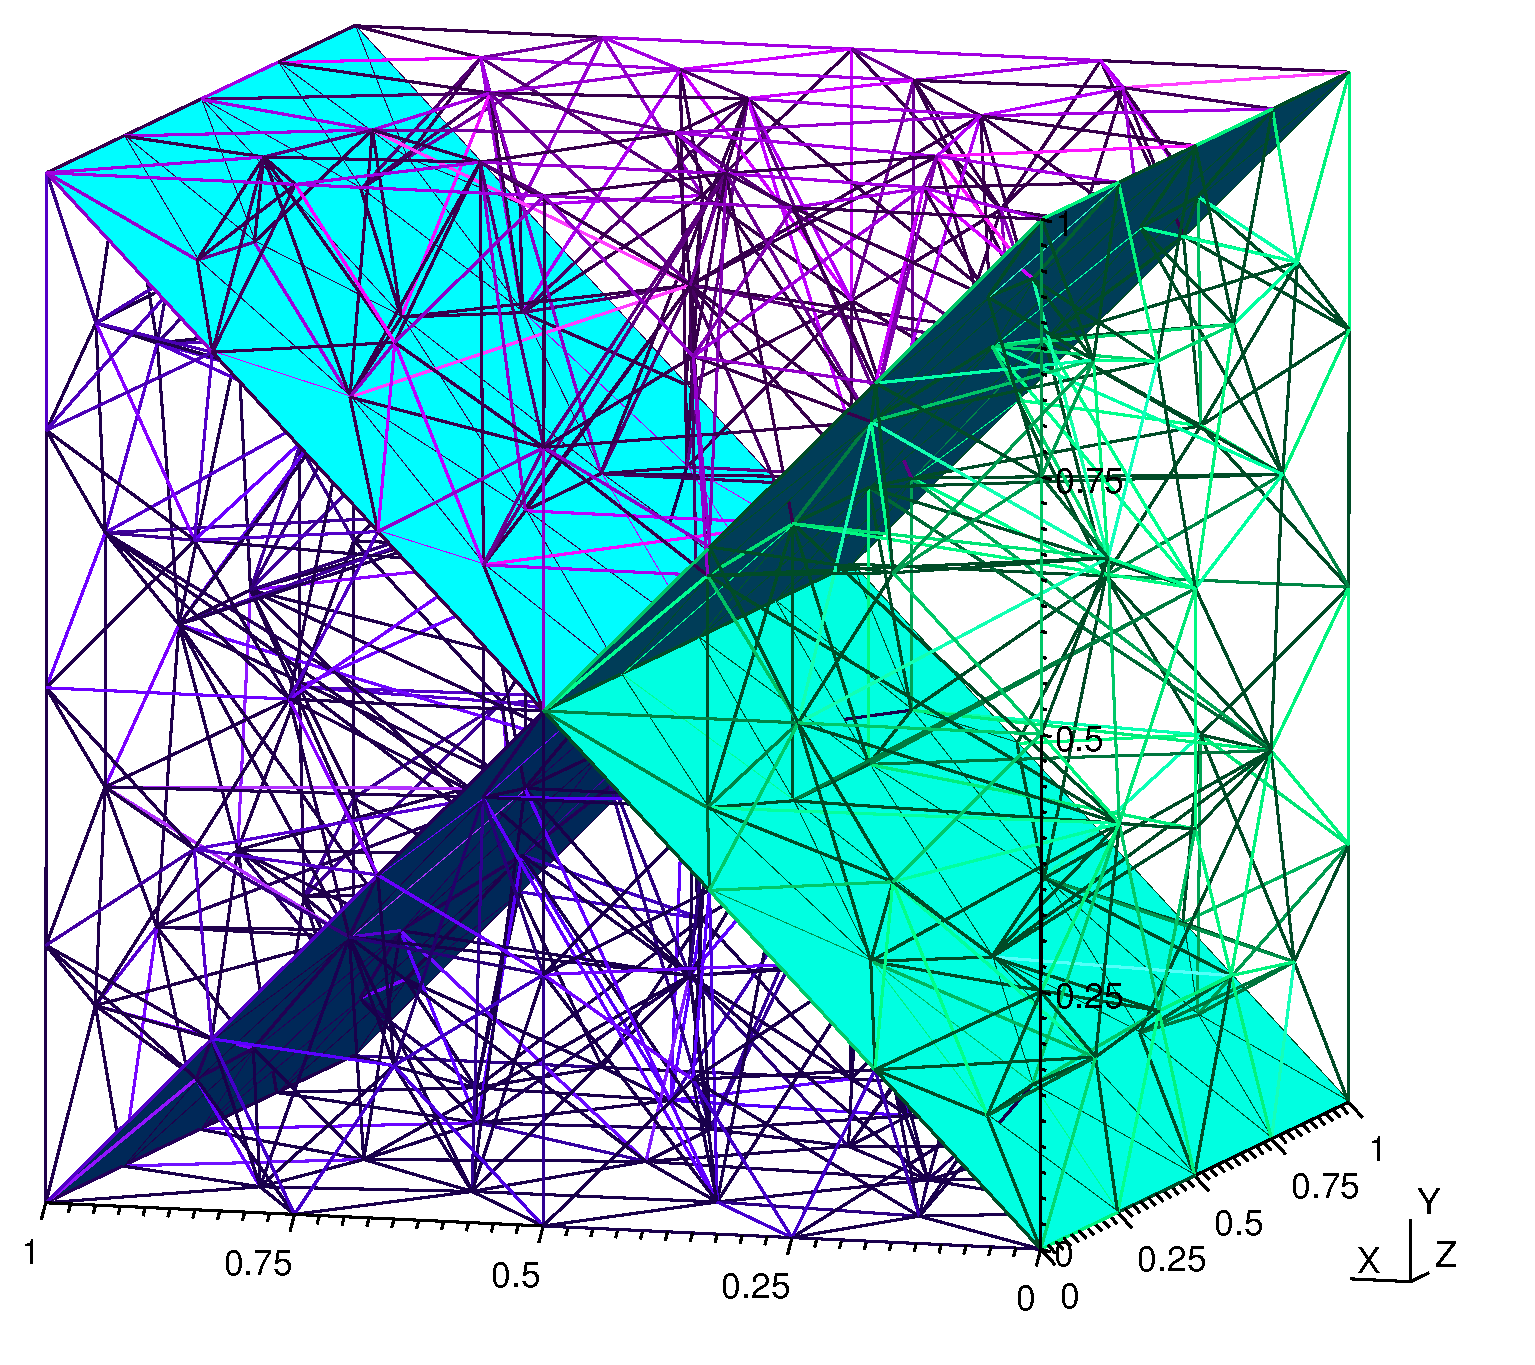
\includegraphics[width=13cm]{tests_graphics/01_mesh.pdf}
\caption{Test 01 -- mesh}
\label{fig:test1_mesh}
\end{figure}
%
%
\subsection*{Parameters}
\begin{itemize}
  \item \textbf{Cross section area:} 1D channel is set to 1.0~\unitss{}{2}{}.
  \item \textbf{Thickness:} 2D fractures are set to 1.0~\unitss{}{1}{}.
  \item \textbf{Conductivity:} The conductivity of materials:
    \begin{itemize}
      \item 1D channel is set to $K=10$~\unitss{}{1}{-1}.
      \item 2D fractures are set to $\mathbf{K}=\left(\begin{array}{cc} 1 & 0 \\ 0 & 1\end{array} \right)$~\unitss{}{1}{-1}.
      \item cube material is set to $\mathbf{K}=\left(\begin{array}{ccc} 0.1 & 0 & 0 \\ 0 & 0.1 & 0 \\ 0 & 0 & 0.1\end{array} \right)$~\unitss{}{1}{-1}.
    \end{itemize}
  \item There is no transport so there are not any other parameters.
\end{itemize}

\subsection*{Verification}
This test verifies solving steady Darcy flow by the mixed hybrid method. There are different dimensional connections 
which are 2D-3D connection between the cube and the flat fractures and 1D-2D connection between the 1D channel 
and the two flat fractures in their crossection. 

Following will not be commented in other examples and use of the functionalities will be considered apparent. No special test
programs are needed to test these as these are partially checked in the unit tests.

The input files \verb'flow_gmsh.con' and \verb'flow_vtk.con' give the same result, however the output is written in different 
formats. Also one can find an example of region set in \verb'flow_gmsh.con'.

Setting a Dirichlet boundary condition using piezometric head values is used in the input file \verb'flow_vtk_piezo.con'.
One can also notice using of the boundary set \verb'BOUNDARY' in this file. We use \emph{FieldFormula} to prescribe boundary
condition so this type of field and the function parser are also verified.

The remaining two files \verb'flow_old_vtk.con' and \verb'flow_vtk_fbc.con' use the obsolete way of defining boundary conditions.
The first one uses the old mesh without any named regions and the boundary condition file \verb'.fbc'. The second one combines
new mesh with named regions and the boudanry condition file created the old way. These tests ensure partially the backward 
compatibility of Flow123d with older input files.

%=====================================================
%                   TEST  2
%=====================================================

\section{Test 02 -- Steady flow in 2D and transport}
\label{sec:test02}
This test involves steady Darcy flow in 2D, connections of 1D-2D elements, Dirichlet boundary condition for flow and transport, 
transport of two substances with zero initial condition for concentration. There are actually two different cases computed in this test. 
Dual porosity and sorption features are present in the explicit transport. Dispersion is defined in the implicit transport.

The coefficient of diffusive transfer through a fracture (means between the fracture and the surrounding material) is set to 
zero so the substance cannot be diffused through the fracture's boundary.

  \begin{itemize} 
    \item \emph{problem type} -- sequential coupling 
    \item \emph{primary equation} -- steady mixed hybrid
    \item \emph{secondary equation} -- transport operator splitting (explicit), discontinuous Galerkin method (implicit)
  \end{itemize}

\subsection*{Geometry and boundary conditions}
The domain is two-dimensional slice through a part of a relief which involves several one-dimensional fractures.

Simple Dirichlet flow boundary condition is defined on left and right side where pressure heads are prescribed. 
There is no flow through the upper and lower boundary of the model. This all causes a flow along the x axis.

Dirichlet boundary condition for transport is prescribed on both sides as it is for flow boundary condition and 
the value of concentration is 1.0~\unitss{1}{-3}{} for both substances. Initial concentration of the substances 
is zero in the whole area. 
%
\begin{figure}[htb!]
\centering
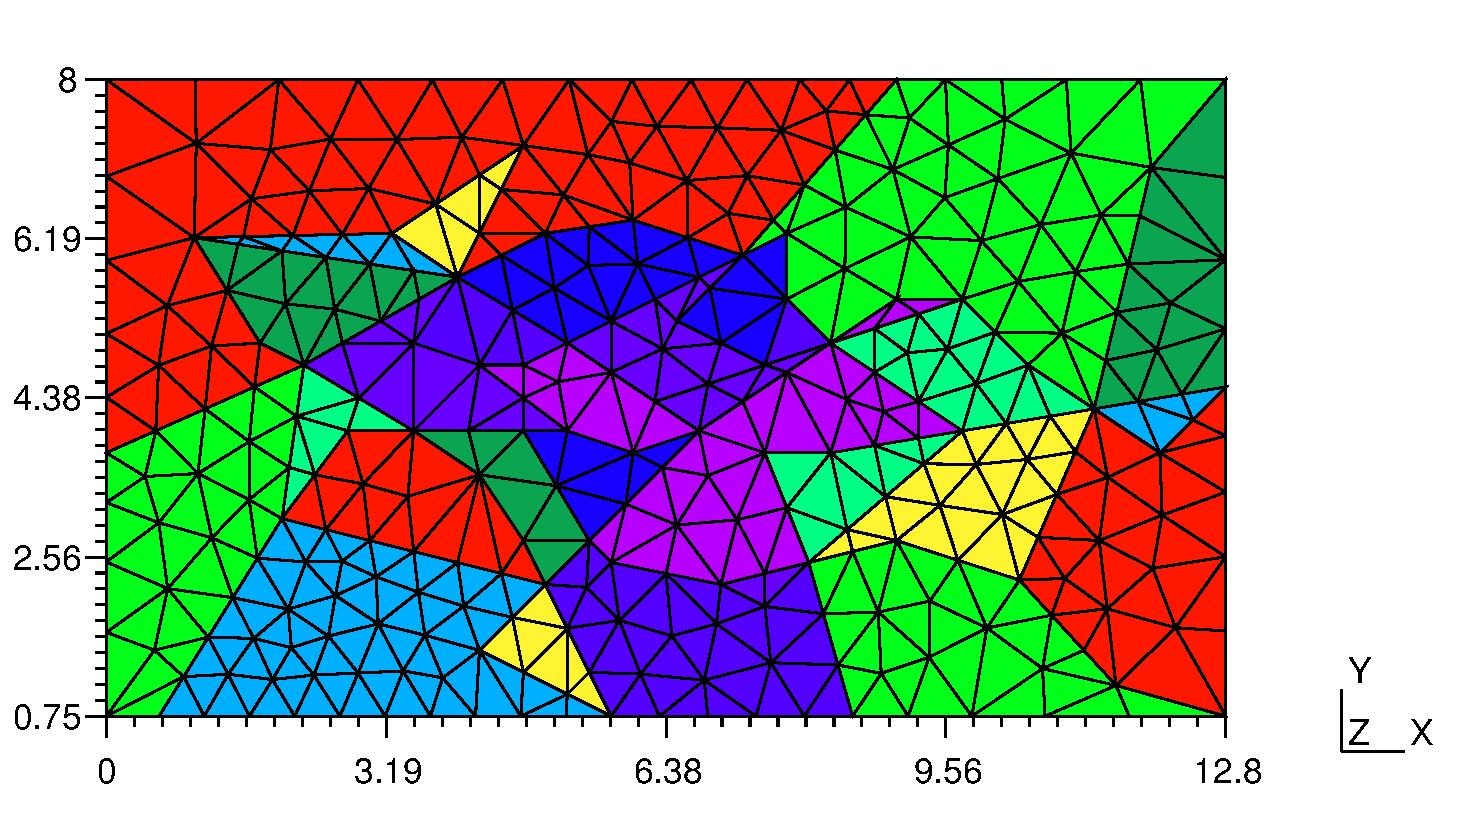
\includegraphics[width=15cm]{tests_graphics/02_mesh.pdf}
\caption{Test 02 -- mesh}
\label{fig:test2_mesh}
\end{figure}
%
%
\subsection*{Parameters}
The flow is steady and the transport is solved in time interval $(0,5.0)$~\unitss{}{}{1}. The output is written every 0.5~\unitss{}{}{1}. 
Time parameters for implicitly computed transport are the same only initial time step is set to 0.5~\unitss{}{}{1}.
\begin{itemize}
  \item \textbf{Cross section area:} 1D fractures are set to 1.0~\unitss{}{2}{}.
  \item \textbf{Thickness:} domain is set to 1.0~\unitss{}{1}{}.
  \item \textbf{Conductivity:} The conductivity of materials:
    \begin{itemize}
      \item fracture material is set to $K=10$~\unitss{}{1}{-1}.
      \item plane material is set to $\mathbf{K}=\left(\begin{array}{cc} 1 & 0 \\ 0 & 1\end{array} \right)$~\unitss{}{1}{-1}.
    \end{itemize}
  \item \textbf{Sorption:} The sorption parameters are for both materials equal:
    \begin{itemize}
      \item linear sorption isotherm parameter of the first substance is set to $k_l=0.02$.
      \item Freundlich sorption isotherm parameters of the second substance are set to $k_F=0.02$, $\alpha=0.5$  
    \end{itemize}
  \item \textbf{Dual porosity:} The dual porosity parameters are for both materials equal:
    \begin{itemize}
      \item mobile porosity coefficient is set to $0.25$
      \item immobile porosity coefficient is set to $0.25$
      \item nonequilibrium coefficient of both substances $0.01$
    \end{itemize}
  \item \textbf{Dispersion coefficients:} No dispersion is involved.
\end{itemize}

\subsection*{Verification}
This test verifies explicitly computed transport considering only convection with dual porosity and sorption and implicitly 
computed transport considering both convection and dispersion. Transport through 1D-2D element connections is computed in addition to the first test.



%=====================================================
%                   TEST  03
%=====================================================

\section{Test 03 -- Steady flow in 2D and transport}
\label{sec:test03}
This test differs from the previous one only by simpler structure of its geometry. It shows how the substace flows in the main fracture and divides in two other fractures. The substance spreads in the fractures much faster in comparision to transport in the plane.
\subsection*{Geometry and boundary conditions}
There is a plane with side 1.0 which is cutted by fractures. The main fracture divides in two other fractures.
\subsection*{Parameters}
The flow is steady and the transport is solved in time interval $(0,1.0)$. The output is written every 0.01. Initial time step for transport computed implicitly is set to 0.1 and the output is written every 0.1.

Other parameters are the same as in test 02.
\subsection*{Verification}
This test verifies the same features as the test 02 does but on a simpler geometry.



%=====================================================
%                   TEST  05
%=====================================================

\section{Test 05 -- Darcy flow boundary conditions}
\label{sec:test05}
There are three types of boundary conditions -- Dirichlet, Neumann and Robin that are tested. All three test have the same geometry and boundary conditions are derived from the same analytical solution.

We will prescribe analytical solution $u=xy$ of Laplace equation $-\Lapl{}u = 0$.
\begin{itemize} 
    \item \emph{problem type} -- sequential coupling 
    \item \emph{primary equation} -- steady mixed hybrid
  \end{itemize}

\subsection*{Geometry and boundary conditions}
The geometry is simple -- square plane in xy coordinates with corner points [0,0] and [1,1]. Each side has its own boundary regions called \verb0.bc_south0, \verb0.bc_east0, \verb0.bc_north0, \verb0.bc_west0.

\textbf{Dirichlet test.} All sides have pressure prescribed. These are south: $u_D=0$; east: $u_D=y$; north: $u_D=x$; west: $u_D=0$.

\textbf{Neumann test.} Two sides have pressure prescribed for the Dirichlet boundary condition: east: $u_D=y$; west: $u_D=0$. Two other sides have flux prescribed: south: $q_N=x$; north $q_N=-x$.

\textbf{Robin test.} Two sides have pressure prescribed  for the Dirichlet boundary condition: east: $u_D=y$; west: $u_D=0$.
For Robin boundary condition we get from the equation boundary pressure
\begin{equation} 
u_R=\frac{1+\sigma_R}{\sigma_R}x. 
\end{equation}
We choose $\sigma_R=0.5$ and then we get $u_R=-2x$ on the south side and $u_R=3x$ on the north side. 

\subsection*{Parameters}
\begin{itemize}
  \item \textbf{Conductivity:} on region \verb0plane0 is $1.0$~\unitss{}{1}{-1}.
  \item \textbf{Thickness:} on region \verb0plane0 is by default 1.0~\unitss{}{1}{}.
  \item There are no other regions, no transport so there are not any other parameters.
\end{itemize}

\subsection*{Verification}
This test verifies prescribing different types boundary conditions.


%=====================================================
%                   TEST  06
%=====================================================

\section{Test 06 -- Coupling between dimensions in Darcy flow}
\label{sec:test06}
There are two tests -- \verb'flow_32d.con' for compatible coupling between 3D-2D and \verb'flow_21d.con' for compatible coupling between 2D-1D.

\begin{itemize} 
    \item \emph{problem type} -- sequential coupling 
    \item \emph{primary equation} -- steady mixed hybrid
  \end{itemize}

We will discuss both the geometry and parameters at once.

%
\begin{figure}[h!]
\centering
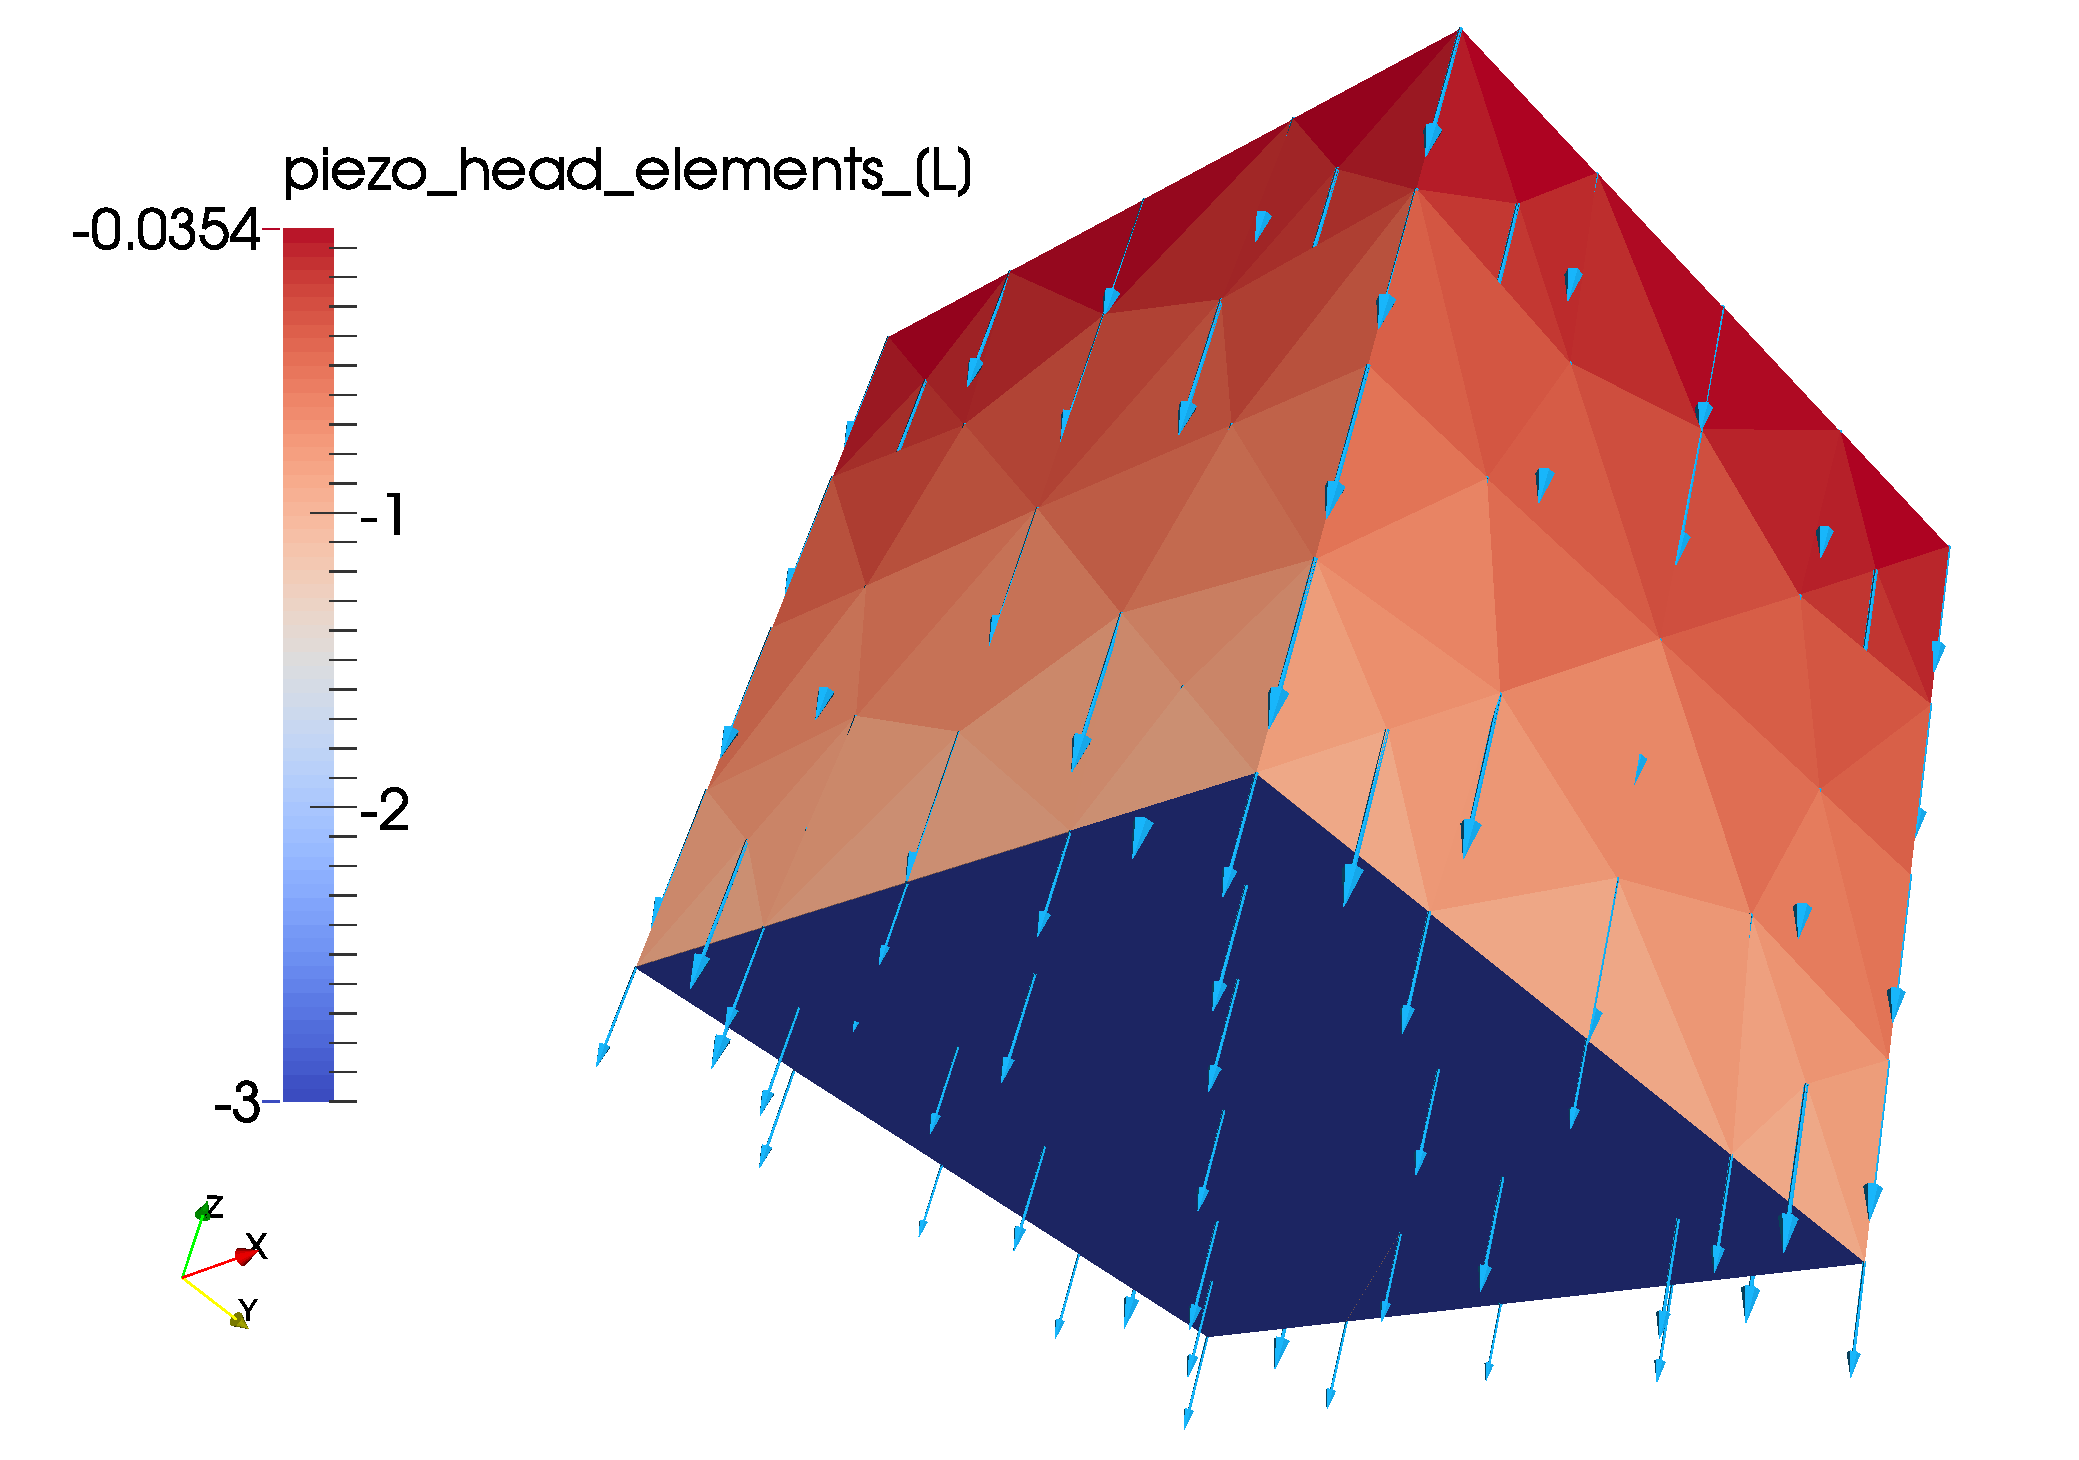
\includegraphics[width=0.6\textwidth]{tests_graphics/06_result_32d.pdf}
\caption{Test 06 -- solution. For verification see the blue plate where the constant piezometric head is.}
\label{fig:test6_solution_32d}
\end{figure}
%
\textbf{3D-2D.}
There is a cube with vertices [0,0,0] [-1,-1,-1] which couples with a 2D crack in the bottom (i.e. $z=-1$~\unitss{}{1}{}).
We consider solution of the piezometric head in the cube $p_3(x,y,z) = z$. We will use it to prescribe Dirichlet boundary condition on the non-coupling parts of the cube.
There are no sources of a flow in the cube. 
We can write the outflow through the bottom of the cube in following term $q_{32} = \mathbf{q_3} \cdot \mathbf{n} = (- K_3 \nabla p_3(x,y,-1))\cdot \mathbf{n}$,
where $\mathbf{n}=(0,0,-1)$.
To obtain Laplace equation with zero right hand side on the 2D crack, we prescribe a new source term (\ref{eqn:test06_f2}) that eliminates the inflow coming from the cube.         
\begin{eqnarray}
    F_2 &=& \delta_2  f_2 + q_{32} = 0   \nonumber\\
    f_2(x,y) &=& -\frac{q_{32}}{\delta_2}   \label{eqn:test06_f2}.
\end{eqnarray}
When $\delta_2 = 10$~\unitss{}{1}{}, $K_3 = 2$~\unitss{}{1}{-1} are choosed then the source term is equal $f_2 = -0.2$~\unitss{}{}{-1}.
Homogenous Neumann condition is prescribed on the boundary of the fraction (zero outflow and inflow).

From the flow coupling equation we can get the piezometric head (\ref{eqn:test06_p2}) on the crack which we can verify.
\begin{eqnarray} 
     \sigma_{32}  ( p_3(x,y,-1) - p_2(x,y) ) &=& q_{32} \nonumber\\
     p_2(x,y) &=& -\frac{q_{32}}{\sigma_{32}} + p_3(x,y,-1) \label{eqn:test06_p2}.
\end{eqnarray}   
When $\sigma_{32} = 1$~\unitss{}{}{-1} is set then the piezometric head in the crack is constant and equal $p_2(x,y) = -3$~\unitss{}{1}{}.

%
\begin{figure}[h!]
\centering
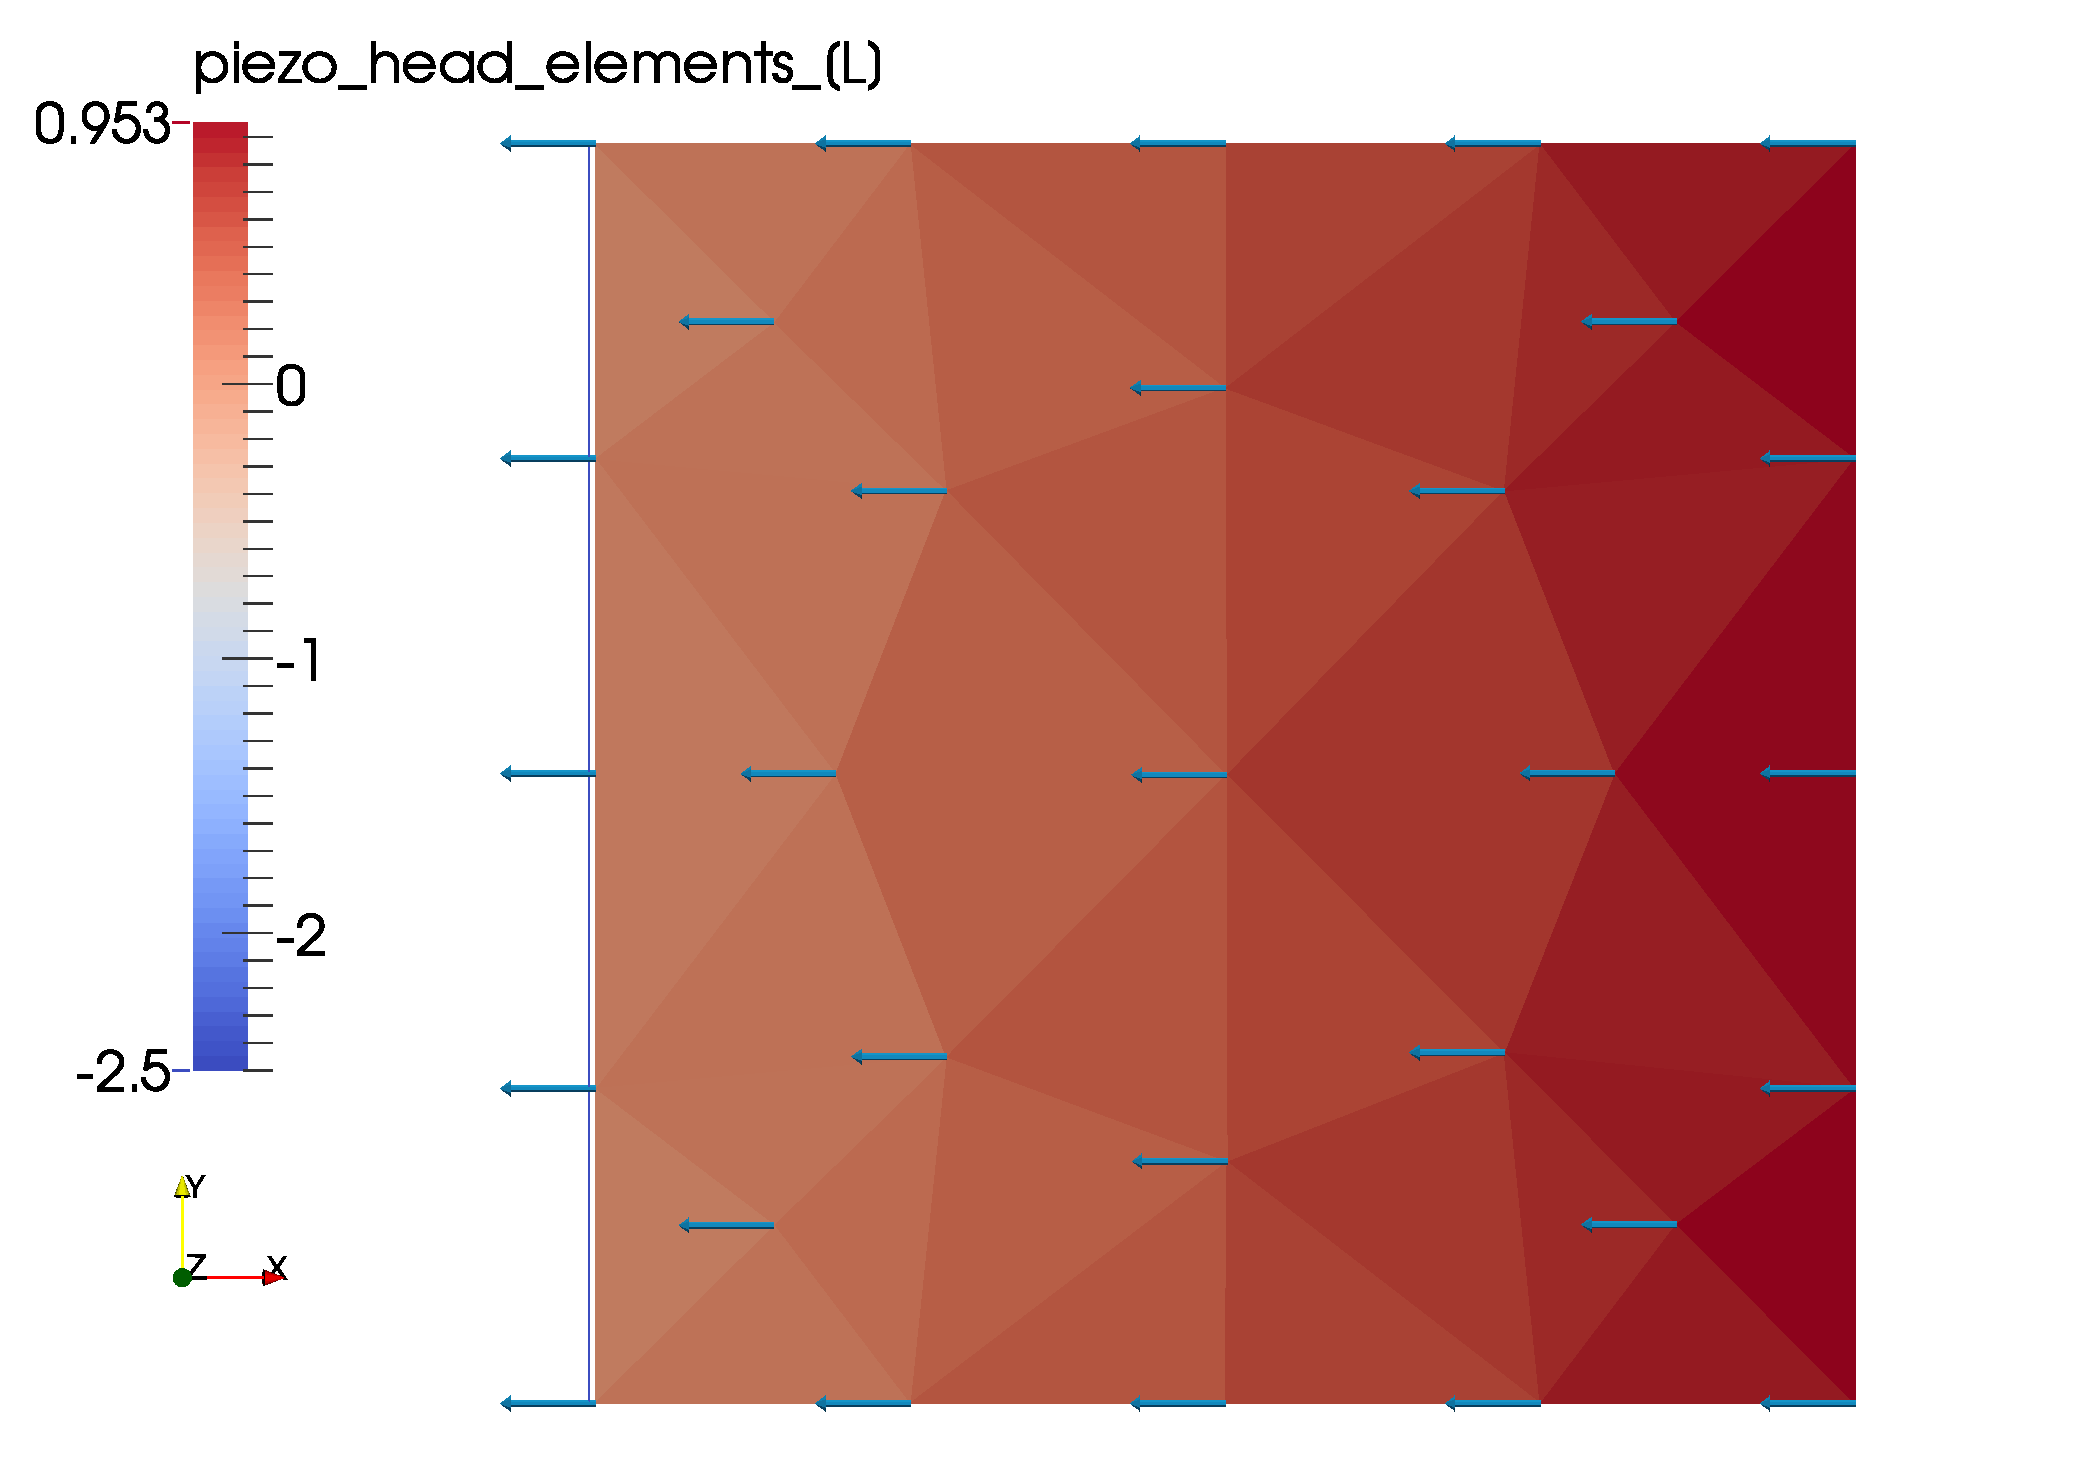
\includegraphics[width=0.6\textwidth]{tests_graphics/06_result_21d.pdf}
\caption{Test 06 -- solution. For verification see the blue channel on the left side of the plane where the constant piezometric head is.}
\label{fig:test6_solution_32d}
\end{figure}
%
\textbf{2D-1D.}
The other tests geometry consists of a 2D crack in $xy$ plane with vertices [0,0] [1,1] and a 1D channel coupling with the crack on the left side ($x=0$). 
Everything is then analogical to the first test.
We consider solution of the pressure in the crack $p_2(x,y) = x$. We will use it to prescribe Dirichlet boundary condition on the non-coupling parts of the crack.
There are no sources of a flow in the crack. 
We can write the outflow through the left side of the crack in the following term $q_{21} = \mathbf{q_2} \cdot \mathbf{n} = (- \delta_2 K_2 \nabla p_2(0,y))\cdot \mathbf{n}$,
where $\mathbf{n}=(-1,0)$.
To obtain Laplace equation with zero right hand side on the channel, we prescribe a new source term (\ref{eqn:test06_f1}) that eliminates the inflow coming from the crack.         
\begin{eqnarray}
    F_1 &=& \delta_1  f_1 + q_{21} = 0   \nonumber\\
    f_1(x,y) &=& -\frac{q_{21}}{\delta_1}   \label{eqn:test06_f1}.
\end{eqnarray}
When $\delta_1 = 20$~\unitss{}{2}{}, $\delta_2 = 10$~\unitss{}{1}{} and $K_2 = 5$~\unitss{}{1}{-1} are choosed then the source term is equal $f_2 = -2.5$~\unitss{}{}{-1}.
Homogenous Neumann condition is prescribed on the boundary of the fraction (zero outflow and inflow).

From the flow coupling equation we can get the pressure (\ref{eqn:test06_p1}) on the plane which we can verify.
\begin{eqnarray} 
     \delta_2 \sigma_{21} ( p_2(0,y) - p_2(y) ) &=& q_{21} \nonumber\\
     p_1(y) &=& -\frac{q_{21}}{\delta_2 \sigma_{21}} + p_2(0,y) \label{eqn:test06_p1}.
\end{eqnarray}   
When $\sigma_{21} = 1$~\unitss{}{}{-1} is set then the pressure in the crack is constant and equal $p_1(y) = -2.5$~\unitss{}{1}{}.

% \subsection*{Parameters}
% Parameters where discussed above.

\subsection*{Verification}
This test verifies correct communication between dimensions 3D-2D and 2D-1D in compatible coupling.
We can also observe the results in the \verb'water_balance' file. We should see that all the inflow 
to the cube should be fully compensated by the negative source. Homogenous Neumann boundary condition 
is prescribed on the crack so there should be no outflow or inflow through the boundary of the crack.
The situation in the second test is similar. The inflow to the crack should be fully compensated by 
the negative source in the channel which should have no other inflow or outflow.


%=====================================================
%                   TEST  8
%=====================================================

\section{Test 08 -- Steady Darcy flow with source}
\label{sec:test08}
This test is aimed at verifying steady Darcy flow with source which is prescribed by function formula. 
We will solve Laplace equation $-\Lapl{}u = f$ where source $f$ is prescribed by function $f = 2(1-y^2) + 2(1-x^2)$.
We can easily prove that (\ref{eqn:test8}) is the analytic solution by replacing it in the Laplace equation.
\begin{equation}
u = (1-x^2)(1-y^2) \label{eqn:test8}
\end{equation}

  \begin{itemize} 
    \item \emph{problem type} -- sequential coupling 
    \item \emph{primary equation} -- steady mixed hybrid
  \end{itemize}

\subsection*{Geometry and boundary conditions}
The domain is a square with opposite vertices $[-1,-1]$ and $[1,1]$. Zero dirichlet boundary condition is prescribed 
on all boundaries -- along the circumference of the square.
 
\subsection*{Parameters}
\begin{itemize}
  \item \textbf{Conductivity:} The conductivity of plane material is $1.0$~\unitss{}{1}{-1}.
  \item There are no other materials, no transport so there are not any other parameters.
\end{itemize}
%
\begin{figure}[h!]
\centering
\includegraphics[width=0.8\textwidth]{tests_graphics/08_result.pdf}
\caption{Test 08 -- solution. Distribution of the pressure matches the analytical solution (\ref{eqn:test8}).}
\label{fig:test8_solution}
\end{figure}
%
\subsection*{Verification}
The solution (pressure) is a paraboloid with a top in $[0,0,1]$ as we can see in the figure \ref{fig:test8_solution}. 
One can verify the equality in Paraview using the prepared state file.


%=====================================================
%                   TEST  10
%=====================================================

\section{Test 10 -- Unsteady flow in 2D}
\label{sec:test10}
Unsteady flow in 2D domain is simulated in this test and is computed by both mixed hybrid and 
lumped mixed hybrid method. No transport is involved. 

\begin{itemize} 
    \item \emph{problem type} -- sequential coupling
    \item \emph{primary equation} -- unsteady mixed hybrid, unsteady lumped mixed hybrid
  \end{itemize}

\subsection*{Geometry and boundary conditions}
The domain is a square with oposite vertices $[0,0]$ and $[1,1]$. Different Dirichlet boundary condition for 
pressure is prescribed on two opposite sides -- 0.0~\unitss{}{1}{} on the left and 100.0~\unitss{}{1}{} on the right.

\subsection*{Parameters}
The flow is solved in time interval $(0,0.5)$ with step 0.01~\unitss{}{}{1}. The output is written every 0.1~\unitss{}{}{1}.
\begin{itemize}
  \item \textbf{Conductivity:} The conductivity of plane material is $0.02$~\unitss{}{1}{-1}.
  \item Initial pressure is set to zero everywhere.
  \item There are no other materials, no transport so there are not any other parameters.
\end{itemize}

\subsection*{Verification}
This test verifies two different numerical methods -- the problem is computed by both mixed hybrid and lumped mixed hybrid method.

%=====================================================
%                   TEST  11
%=====================================================

\section{Test 11 -- Radioactive decay chain with more branches}
8 isotopes are members of considered decay chain with three branches. Transport boundary conditions does not matter 
because zero presure gradient is considered. Final concentrations of all isotopes except C decrease to zero after 20 
time steps, whereas C concentration grows to 0.36.
\[
 E\xrightarrow{}D\xrightarrow{}F\xrightarrow{}B
 \quad
 \begin{matrix}
    0.2B\xrightarrow{}A & A\xrightarrow{}G \\
    0.6B\xrightarrow{}H & H\xrightarrow{}G \\
    0.2B\xrightarrow{}G &\\
 \end{matrix}
 \quad
 G\xrightarrow{}C 
\]

\begin{itemize} 
    \item \emph{problem type} -- sequential coupling
    \item \emph{primary equation} -- steady mixed hybrid
    \item \emph{secondary equation} -- transport operator splitting
    \item \emph{reactions} -- linear reactions
  \end{itemize}

\subsection*{Geometry}
The domain is a prism which base is a right-angled triangle with its ordinates 3.0~\unitss{}{1}{}. 
There are only three tetrahedron elements in the mesh.

\subsection*{Parameters}
The flow is steady and the transport is solved in time interval $(0,10.0)$~\unitss{}{}{1}. The output is written every 0.5~\unitss{}{}{1}.

Half-lives are equal to 0.5 for all isotopes. Initial concentrations are summarized in the table below:
  \begin{center}
    \begin{tabular}[c]{|l|c|c|c|c|c|c|c|c|}
      \hline
      isotop & A & B  & C & D & E & F & G & H \\[4pt]
      initial concentration & 0.01 & 0.02 & 0.03 & 0.04 & 0.05 & 0.06 & 0.07 & 0.08 \\[4pt]
      \hline
    \end{tabular}
  \end{center}


\subsection*{Verification}


%=====================================================
%                   TEST  12
%=====================================================

\section{Test 12 -- Radioactive decay}
There are actually two tests of the radioactive decay. The first one considers first order reaction of two isotopes 
determined by kinetic constant and the other one describes radioactive decay chain of three isotopes.

\begin{itemize} 
    \item \emph{problem type} -- sequential coupling
    \item \emph{primary equation} -- steady mixed hybrid
    \item \emph{secondary equation} -- transport operator splitting
    \item \emph{reactions} -- linear reactions
  \end{itemize}

\subsection*{Geometry and boundary conditions}
The domain is a prism which base is a right-angled triangle with its ordinates 3.0 units long. There are then only three tetrahedron elements in the mesh.

There are two Dirichlet boundary conditions for flow prescribed.

\begin{itemize}
  \item \textbf{Conductivity:} The conductivity of the prism material is $0.01$~\unitss{}{1}{-1}. 
  \item There is no other parameter for flow or transport.
\end{itemize}



\subsection{First order reaction determined by kinetic constant}
The only linear reaction between D and F substances.
\[
D\xrightarrow{k}F
\]

\subsection*{Parameters}
The flow is steady and the transport is solved in time interval $(0,10.0)$. The output is written every 0.5~\unitss{}{}{1}.  
\begin{itemize}
  \item \textbf{Substances:} 6 substances to be transported -- A, B, C, D, E, F
  \item \textbf{Kinetic constant:} $k = 0.277258872$
\end{itemize}

\subsection*{Verification}

\subsection{Radioactive decay chain}
The considered radioctive decay chain is:
\[
 D\xrightarrow{t_{1/2,D}}F\xrightarrow{t_{1/2,F}}B
\]
\subsection*{Parameters}
Time parameters are the same as they are above.
\begin{itemize}
  \item \textbf{Substances:} 6 substances to be transported -- A, B, C, D, E, F
  \item \textbf{Decay half-lives:} $t_{1/2,D} = t_{1/2,F} = 2.5$
\end{itemize}

\subsection*{Verification}

% Both following tests are realized without combination with transport (zero pressure gradient).
% verification of:
% - first order reaction A->B determined by kinetic constant,
% -- 6 chemical species (A, B, .., F) are transported but just 2 of them take a part in considered first order kinetic reaction wich looks as follows
% --- D->F, appropriate kinetic constant is k = 0.277258872.
% --- Initail conditions look as follows, A(0) = 0.01, B(0) = 0.02, C(0) = 0.03, D(0) = 0.04, E(0) = 0.05, F(0) = 0.06.
% --- Transport boundary conditions does not matter because zero presure gradient is considered.
% --- Final concentrations of all isotopes except A, B, C, E do not change. Concentrations of D decreases to 0.003. Concentration of F increase to 0.85 in 20 time steps.

% - narrow radioctive decay chain without branches, A -> B -> C,
% -- 6 isotopes (A, B, .., F) are transported but just 3 of them are members of considered decay chain which looks as folows
% --- D->F->B
% --- Initail conditions look as follows, A(0) = 0.01, B(0) = 0.02, C(0) = 0.03, D(0) = 0.04, E(0) = 0.05, F(0) = 0.06.
% --- Transport boundary conditions does not matter because zero presure gradient is considered.
% --- Final concentrations of all isotopes except A, C, E do not change. Concentrations of D and B decrease to 0.004 and 0.012 respectively. Concentration of B increase to 0.1 in 20 time steps.

%=====================================================
%                   TEST  13
%=====================================================

\section{Test 13 -- Solute mixing on the edge}
This test realizes mixing of substances on the edges of planes and also does quantitative test on a trivial 
transport problem. The problem is computed with both explicit and implicit transport.

\begin{itemize} 
    \item \emph{problem type} -- sequential coupling 
    \item \emph{primary equation} -- steady mixed hybrid
    \item \emph{secondary equation} -- transport operator splitting (explicit), discontinuous Galerkin method (implicit)
  \end{itemize}

\subsection*{Geometry and boundary conditions}
The domain is a fork where the main branch with the incoming solute is 5~\unitss{}{1}{} long and lies in 
the $xy$ plane. Then it is divided into two other branches $5\sqrt{2}$~\unitss{}{1}{} long, one with 
positive and the another with negative $z$ coordinate. There are different conductivities in each branch.

Dirichlet boundary conditions for flow and transport are prescribed at the beginning of the main 
plane ($x=0$~\unitss{}{1}{}) and at the ends of the secondary branches ($x=10$~\unitss{}{1}{}).

flow: $h_D=-x-z+10.0$ which gives 10.0~\unitss{}{1}{} at point [0,0,0] and $\pm5$~\unitss{}{1}{} at points [10,0,$\mp5$]\\
transport: concentration is 1.0 at point [0,0,0] and 0.0 at points [10,0,$\mp5$]

Initial concentration of the substances is zero in the whole area. 
%
\begin{figure}[htb!]
\centering
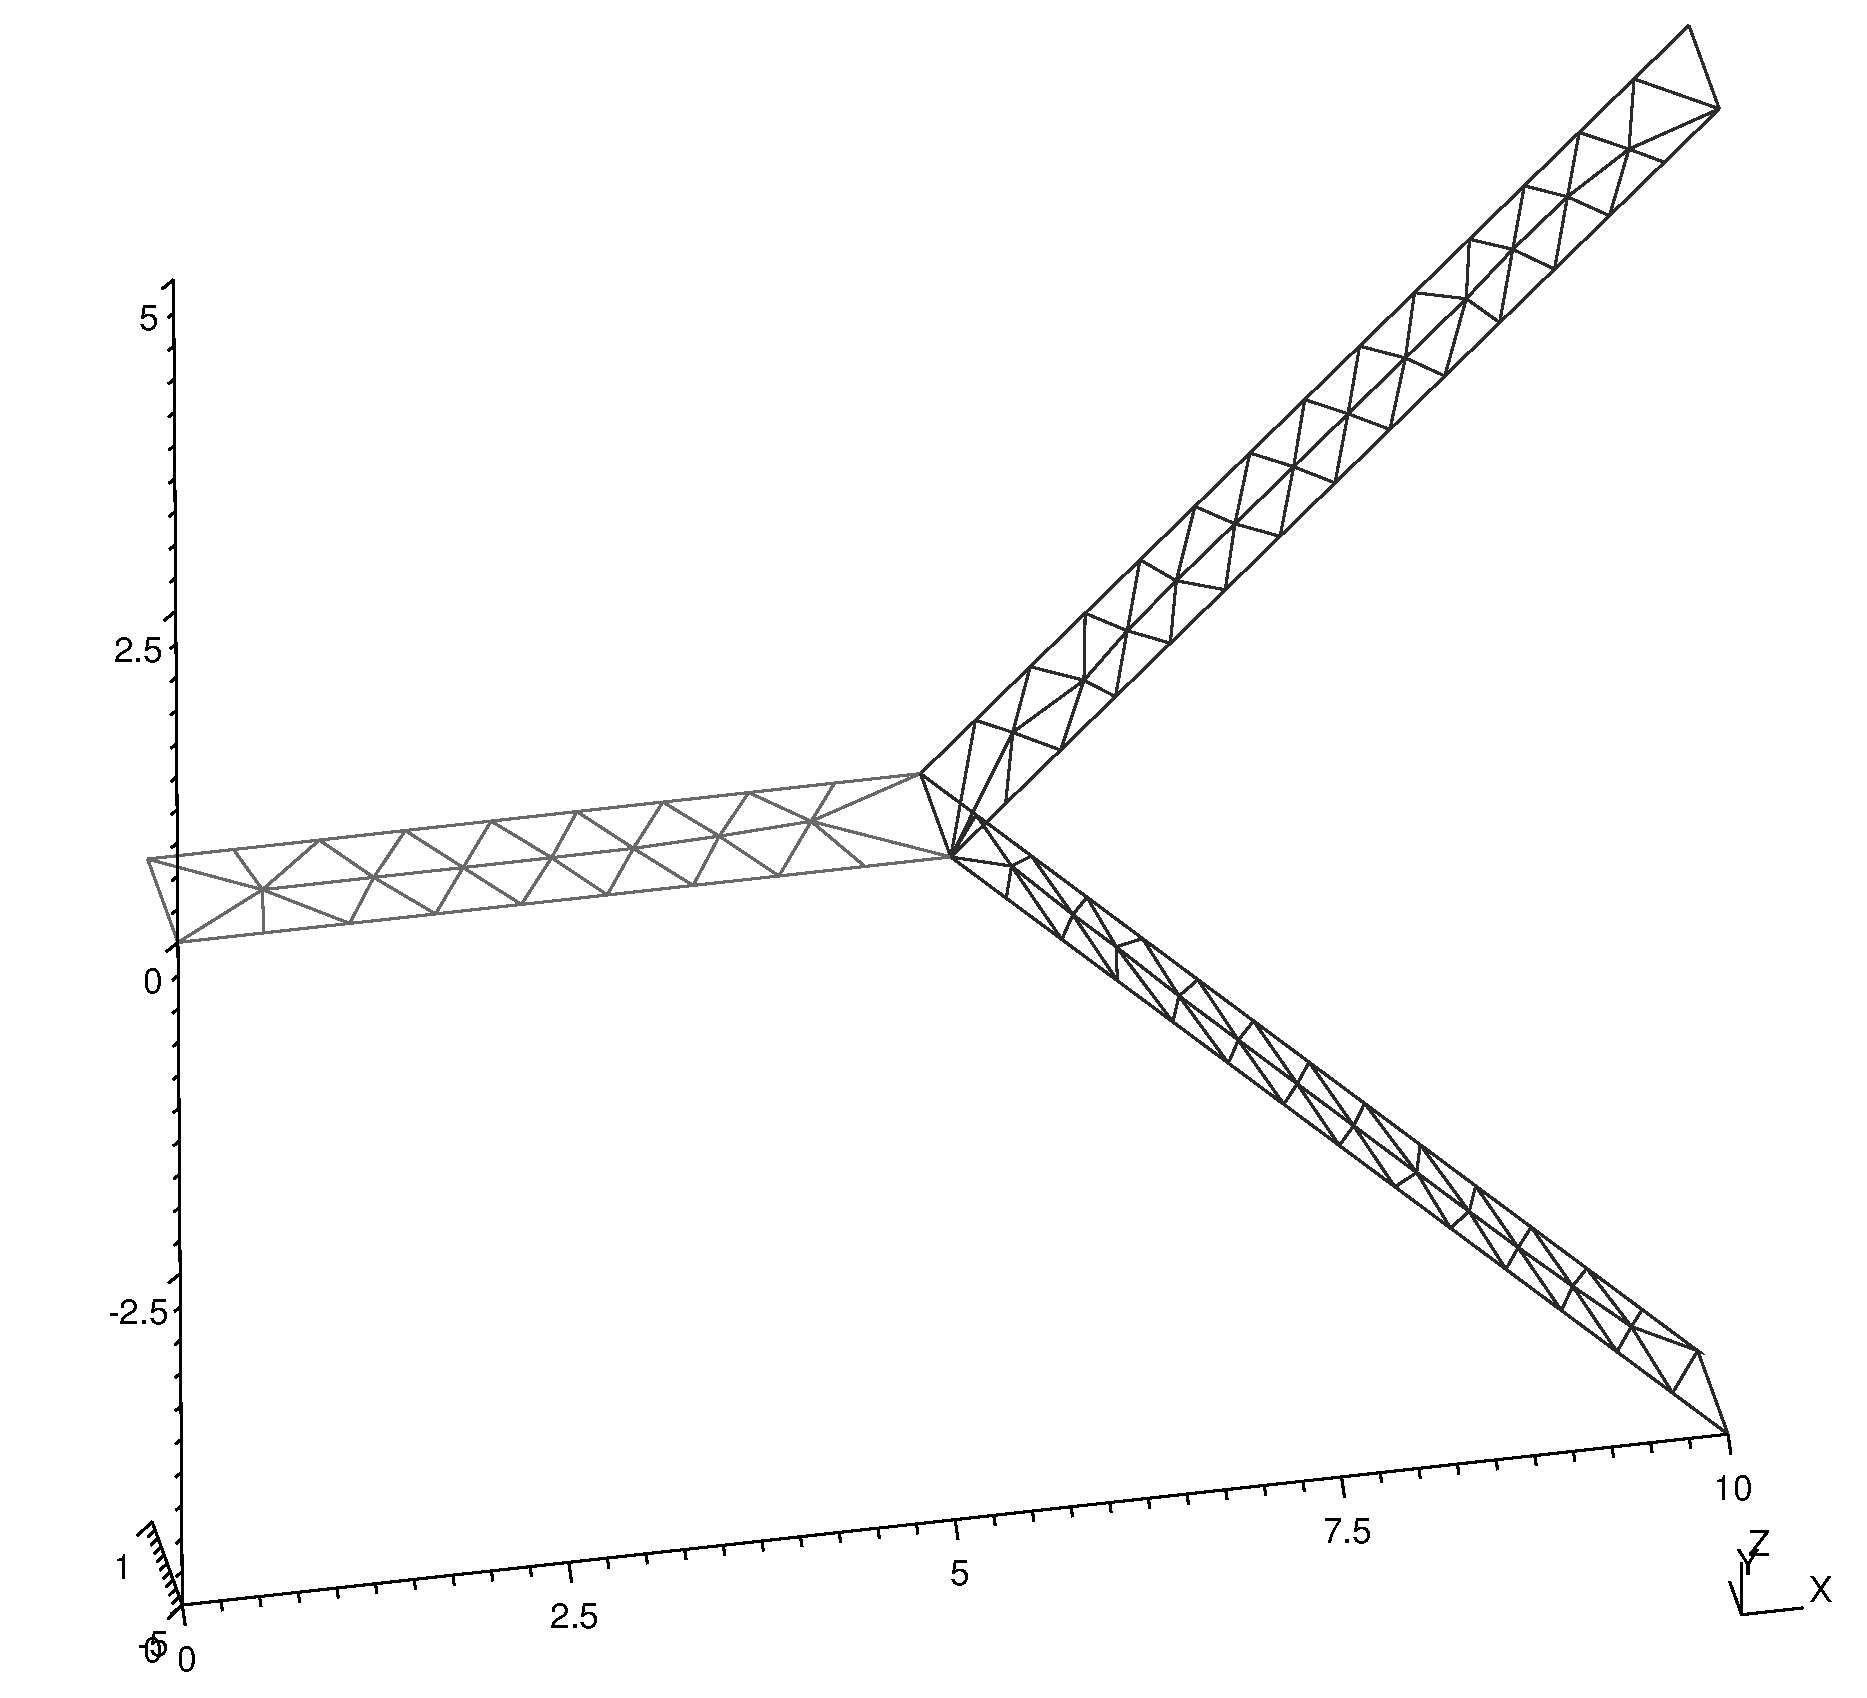
\includegraphics[width=12cm]{tests_graphics/13_mesh.pdf}
\caption{Test 13 -- mesh}
\label{fig:test13_mesh}
\end{figure}
%
%
\subsection*{Parameters}
The flow is steady and the transport is solved in time interval $(0,100.0)$~\unitss{}{}{1}. 
The output is written every 0.5~\unitss{}{}{1}. 
Time parameters for implicitly computed transport are the same only initial time step and output time is set to 5.0~\unitss{}{}{1}.
\begin{itemize}
  \item \textbf{Thickness:} all planes are set to 1.0~\unitss{}{1}{}.
  \item \textbf{Conductivity:} The conductivity of materials (isotropic planes):
    \begin{itemize}
      \item main branch (material num. 17): $K=1$~\unitss{}{1}{-1}.
      \item branch (positive $z$, material num. 18): $K=0.1$~\unitss{}{1}{-1}.
      \item branch (negative $z$, material num. 19): $K=0.1$~\unitss{}{1}{-1}.
    \end{itemize}
  \item \textbf{Dispersion coefficients:} Default parameters are set in implicit transport, so no dispersion is present. 
        For more details see \hyperlink{IT::TransportDG-BulkData}{TransportDG\_BulkData} in the input reference.
\end{itemize}

\subsection*{Verification}
This test verifies qualitatively both the problem of flow and transport.

%=====================================================
%                   TEST  14
%=====================================================

\section{Test 14 -- Variable transport boundary condition}
We consider a time variable boundary condition for transport in this test. Steady flow with constant velocity is caused by a pressure 
gradient from one side of a 2D strip to the another. Dirichlet boundary condition for transport evolving in time is prescribed on the 
right side using set of older \verb'.tbc' files. 

\begin{itemize} 
    \item \emph{problem type} -- sequential coupling, 
    \item \emph{primary equation} -- steady mixed hybrid
    \item \emph{secondary equation} -- transport operator splitting (explicit), discontinuous Galerkin method (implicit)
  \end{itemize}

\subsection*{Geometry and boundary conditions}

Dirichlet boundary condition for pressure is prescribed $x$ all around the plane and causes constant flow from right to left 
(pressure prescribed on the upper and lower sides are equal along x axis so causes no flow). Transport boundary condition has 
the same prescribtion as for the pressure, only the values evolves in time.

Initial concentration is zero on the whole plane. Two pulses of nonzero concentration are applied on the boundary. The changes 
of the boundary condition at specified times are shown in the following table:
%
\begin{center}
  \begin{tabular}{|l|c|c|c|c|c|}
    \hline
    time \units{}{1}{} & $0$ & $1$ & $3$ & $6$ & $7$\\
    concentration & $0$ & $20$ & $0$ & $40$ & $0$\\
    \hline
  \end{tabular}
\end{center}

\begin{figure}[htb!]
\centering
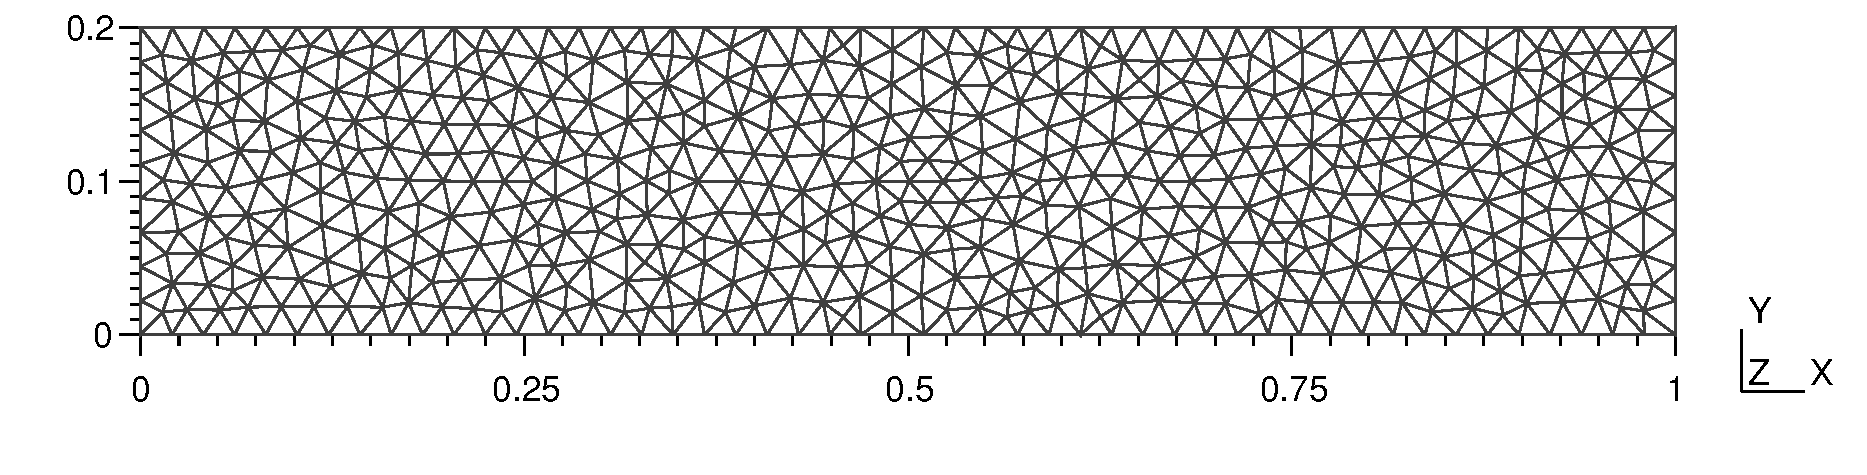
\includegraphics[width=15cm]{tests_graphics/14_mesh.pdf}
\caption{Test 14 -- mesh}
\label{fig:test14_mesh}
\end{figure}
%
%
\subsection*{Parameters}
The flow is steady and the transport is solved in time interval $(0,10.0)$~\unitss{}{}{1}. The output is written every 
1.0~\unitss{}{}{1}. Time parameters for implicitly computed transport are the same only initial time step is set to 1.0~\unitss{}{}{1}.
%
\begin{itemize}
  \item \textbf{Thickness:} all planes are set to 1.0~\unitss{}{1}{}.
  \item \textbf{Conductivity:} The conductivity of material (isotropic plane): $K=0.1$~\unitss{}{1}{-1}.
  \item \textbf{Dispersion coefficients:} Default parameters are set in implicit transport, so no dispersion is present. 
        For more details see \hyperlink{IT::TransportDG-BulkData}{TransportDG\_BulkData} in the input reference.
\end{itemize}
%

\subsection*{Verification}



%=====================================================
%                   TEST  15
%=====================================================

\section{Test 15 -- Unsteady flow with transport}
Transport of a single pulse of concentration moving along a 2D strip is solved. This test involves unsteady flow computed by lumped hybrid method, transport is solved both with explicit and implicit (involves dispersion) scheme.
 
\begin{itemize} 
    \item \emph{problem type} -- sequential coupling, 
    \item \emph{primary equation} -- unsteady lumped mixed hybrid
    \item \emph{secondary equation} -- transport operator splitting (explicit), discontinuous Galerkin method (implicit)
  \end{itemize}

\subsection*{Geometry and boundary conditions}
The domain is a 2D strip with dimensions $1.0$x$16.0$. Zero Dirichlet boundary for flow is prescribed at $x=0$, zero Neumann boundary is elsewhere. 

Dirichlet transport boundary condition is set on the left side to 10.0 only at the beginning. Then is this boundary condition zero.

\subsection*{Parameters}
Initial pressure is zero everywhere. 
The source is prescribed with function $f=-x$ along the strip.
%
\begin{itemize}
  \item \textbf{Thickness:} all planes are set to 1.0~$L$.
  \item \textbf{Conductivity:} The conductivity of material (isotropic plane): $K=1.0$.
  \item \textbf{Source formula:} $f = -x$
  \item \textbf{Diffusivity coefficients:} are used in implicit transport wth dispersion. 
	Default parameters are set ($d_m=1e-6$, others are zero, see manual or parameters in test02 in ~\ref{sec:test02}).
\end{itemize}
%
\begin{figure}[htb!]
\centering
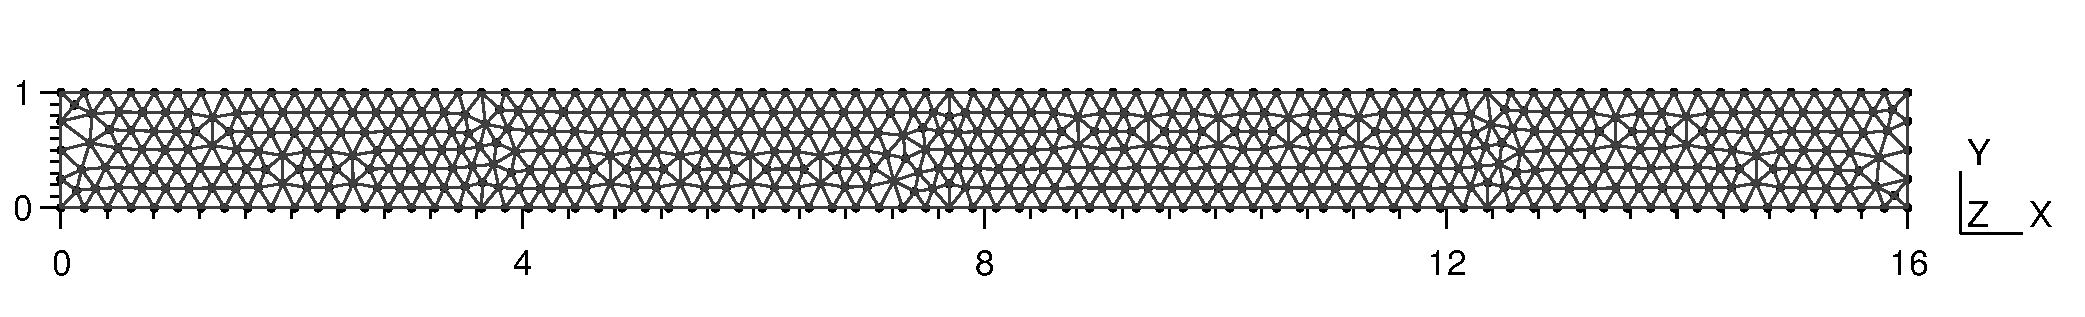
\includegraphics[width=15cm]{tests_graphics/15_mesh.pdf}
\caption{Test 15 -- mesh}
\label{fig:test15_mesh}
\end{figure}
%
%
\subsection*{Verification}
The test is similar to the test 10 but here in addition the computation of a transport in an unsteady flow field is verified.


%=====================================================
%                   TEST  16
%=====================================================

\section{Test 16 -- Substance concentration source in transport}
This test include a source of concentration of a substance. The domain is a 2D strip in vertical direction. There is a steady flow with constant velocity in the vertical direction. Two sources are situated on two elements at the top of the strip and the substance is transported down along the strip. The concentration values of the sources are defined in the \verb0tso0 input file.

\begin{itemize} 
    \item \emph{problem type} -- sequential coupling, 
    \item \emph{primary equation} -- steady mixed hybrid
    \item \emph{secondary equation} -- transport operator splitting
  \end{itemize}

\subsection*{Geometry}


\subsection*{Parameters}

\subsection*{Verification}



%=====================================================
%                   TEST  17
%=====================================================

\section{Test 17 -- Radioactive decay -- Pade approximation}
This test solves radioactive decay chain of five isotopes using Pade approximation.
The considered radioctive decay chain is:
\[
 A\xrightarrow{t_{1/2,A}}B\xrightarrow{t_{1/2,B}}C\xrightarrow{t_{1/2,C}}D\xrightarrow{t_{1/2,D}}E
\]

\begin{itemize} 
    \item \emph{problem type} -- sequential coupling, 
    \item \emph{primary equation} -- steady mixed hybrid
    \item \emph{secondary equation} -- transport operator splitting
    \item \emph{reactions} -- Pade approximation
  \end{itemize}

\subsection*{Geometry}
The geometry and material and transport parameters are the same as in test 12.


\subsection*{Parameters}
\begin{itemize}
  \item \textbf{Substances:} 5 substances to be transported -- A, B, C, D, E
  \item Polynomial degree of the nominator and the denominator of Pade approximation is~3.
  \item \textbf{Decay half-lives:} 
    \begin{tabular}[c]{|c|c|c|c|}
      \hline
      $t_{1/2,A}$ & $t_{1/2,B}$  & $t_{1/2,C}$ & $t_{1/2,D}$\\[4pt]
      $1.3863$ & $2.3105$ & $1.5403$ & $1.1552$\\[4pt]
      \hline
    \end{tabular}
\end{itemize}

\subsection*{Verification}


%=====================================================
%                   TEST  18
%=====================================================

\section{Test 18 -- Diffusion through fractures}
This test is aimed at transport caused just by diffusion. 

There is a triangular domain with zero pressure everywhere so no flow is present. Triangular element with high concentration of a substance lies in the middle of the domain and its sides neighbour with fractures.
The coeffients of molecular diffusion and diffusive transfer through fractures are the parameters of the implicit transport and are set in the configuration file.

\subsection*{Geometry}

\subsection*{Parameters}

\subsection*{Verification}






% ===================  PREPARING  ==================
% \section{Test 20 -- Dirichlet boundary condition}
% \label{sec:test20}
% This test involves steady Darcy flow in 3D determined by Dirichlet boundary condition. The analytic solution is prescribed $u = xyz$. We can see from the formula that there are no sources $-\Lapl{}u = 0$ (zero right hand side) and we can easily define Dirichlet boundary conditions on the sides of the cube just by evaluating the solution there.
% 
% \subsection*{Geometry}
% The domain is a cube with its side 1.0~$L$ long.
% Dirichlet boundary conditions are summarized in the following table. Physical domains corresponds with the numbers in \verb0geo0 file, the row \emph{plane} contains equations of the planes (sides of the cube). The row \emph{Dirichlet} contains solution on the planes. The row \emph{boundary} segment contains numbers of segments defined in \verb0con0 file.
% 
% \begin{center}
%   \begin{tabular}{|l|c|c|c|c|c|c|}
%       \hline
%       boundary segment & 1 & 2 & 3 & 4 & 5 & 6 \\ 
%       physical domain & 27 & 28 & 29 & 30 & 31 & 32 \\ 
%       plane & $z-1=0$  & $x-1=0$ & $z=0$ & $x=0$ & $y-1=0$& $y=0$\\
%       Dirichlet [$u_D$] & $xy$ & $yz$ & $0$ & $0$ & $xz$ & $0$\\
%       \hline
%   \end{tabular}
% \end{center}
% 
% \subsection*{Parameters}
% \begin{itemize}
%   \item \textbf{Conductivity:} cube material is set to $\mathbf{K}=\left(\begin{array}{ccc} 1.0 & 0 & 0 \\ 0 & 1.0 & 0 \\ 0 & 0 & 1.0\end{array} \right)$.
%   \item There is no transport so there are not any other parameters.
% \end{itemize}
% 
% \subsection*{Verification}
% This test verifies prescribing Dirichlet boundary condition.
% 
% 
% \section{Test 21 -- Neumann boundary condition}
% \label{sec:test21}
% This test uses the same geometry and parameters as in the test 20 (viz~\ref{sec:test20}) but there are prescribed both Dirichlet and Neumann boundary conditions. 
% 
% The table of the boundary conditions is below. The row \emph{Dirichlet} contains contains solution on the planes and the row \emph{Neumann} contains flow through the planes.
% 
% \begin{center}
%   \begin{tabular}{|l|c|c|c|c|c|c|}
%       \hline
%       boundary segment & 1 & 2 & 3 & 4 & 5 & 6 \\ 
%       physical domain & 27 & 28 & 29 & 30 & 31 & 32 \\ 
%       plane & $z-1=0$  & $x-1=0$ & $z=0$ & $x=0$ & $y-1=0$& $y=0$\\
%       Dirichlet [$u_D$] 
% 	  &   -   & $yz$ & $0$ & $0$ &   -   & $0$\\
%       Neumann [$-\nabla{}u\cdot{}\mathbf{n}$] 
% 	  & $-xy$ &   -  &  -  &  -  & $-xz$ & - \\
%       \hline
%   \end{tabular}
% \end{center}
% 
% \subsection*{Verification}
% This test verifies prescribing Neumann boundary condition.
% 
% \section{Test 22 -- Newton boundary condition}
% \label{sec:test21}
% This test uses the same geometry and parameters as in the test 20 (viz~\ref{sec:test20}) but there is prescribed Newton boundary condition $-\nabla{}u\cdot{}\mathbf{n} = \sigma(u-u_T)$.
% 
% The table of the boundary conditions where parameters $\sigma$ and $u_T$ are written is below. The values of parameters were chosen to satisfy condition $-\nabla{}u\cdot{}\mathbf{n} = -(yz,xz,xy)\cdot\mathbf{n} = \sigma(u-u_T)$
% 
% \begin{center}
%   \begin{tabular}{|l|c|c|c|c|c|c|}
%       \hline
%       boundary segment & 1 & 2 & 3 & 4 & 5 & 6 \\ 
%       physical domain & 27 & 28 & 29 & 30 & 31 & 32 \\ 
%       plane & $z-1=0$  & $x-1=0$ & $z=0$ & $x=0$ & $y-1=0$& $y=0$\\
%       $-\nabla{}u\cdot{}\mathbf{n}$ & $-xy$ & $-yz$ & $xy$ & $yz$ & $-xz$ &\\
%       $\sigma$ & $xy$ & $yz$ & $0$ & $0$ & $xz$ & $0$\\
%       $u_T$ & $u_T=xy$ & $u=yz$ & $u=0$ & $u=0$ & $u=xz$ & $u=0$\\
%       \hline
%   \end{tabular}
% \end{center}
% 
% \subsection*{Verification}
% This test verifies prescribing Newton boundary condition.


\chapter{Main input file reference}
% support macros



%%%%%%%%%%%%%%%%%%%%%%%%%%%%%%%%%%%%%%%%%%%%%%%%%%%%%%%
% RecordType environment
%
% usage:
% \begin{RecordType}
%       {<record name>}                 % name of the record, used for header and for hypertarget in form IT::<record name>
%       {<parent abstract record>}      % possible parent abstract record
%       {<default conversion key>}      % possible auto conversion key
%       {<link>}                        % possible hyperlink into hand written text
%       {< record description>}         % description of the record
%
%       \KeyItem{<name>}                % name of the key
%               {<type>}                % type of the key 
%               {<default value>}       % type of default value and possibly the value itself
%               {<link>}                %  possible hyperlink to hand written text
%               {<key description>}     % description of the key
%       ...
% \end{RecordType}

\def\AddDoc#1{}

\newenvironment{RecordType}[5]
{
 \ifstrequal{#4}{\relax}{%
    % turn off
    \begingroup
    \gdef\KeyItem##1##2##3##4##5{}
 }{
    \par
    \vskip 2ex
    \hrule%
    \vskip 0.3ex
    \hrule
    \noindent%
    record: {\bf #1}%
    \ifstrempty{#2}{}{ implements abstract type: #2}%
    \ifstrempty{#3}{}{ constructible from key: #3}%
    {#4}
    \par%
    \vskip 0.5ex
    \hrule%
    \vskip 0.3ex
    \hrule
    {#5}
    \begingroup%records of steady field type which we describe right now 
    \addtolength{\leftskip}{3em}%
    %
    \gdef\KeyItem##1##2##3##4##5{%
        \par
        \vskip 0.3ex
        %\hrule%
        \noindent%
        \hspace{-3em}{\bf\tt ##1} = {\it \textless ##2\textgreater}% \hfill \makebox[0.4\textwidth][l]{DEFAULT: {##3}\hfil}%
        \par
        Default: {##3} \hfill [##4]
        \par
        {##5}
    }%
  }
}{%
  \vskip 2ex  
  \endgroup%
}

%%%%%%%%%%%%%%%%%%%%%%%%%%%%%%%%%%%%%%%%%%%%%%%%%%%%%%%
% AbstractType environment
%
% usage:
% \begin{AbstractType}
%       {<record name>}
%       {<default descendant>}
%       {<link>}
%       {<description>}         % Description paragraph of the abstract type.
%       \Descendant{<type name>}
% \end{AbstractType}

\newenvironment{AbstractType}[3]
{\par
 \vskip 2ex
 \hrule%
 \vskip 0.3ex
 \hrule
 \noindent%
 abstract type: {\bf #1}%
 \ifstrempty{#2}{}{ default descendant: #2}%
 \par%
 \vskip 0.5ex
 \hrule%
 \vskip 0.3ex
 \hrule
 #3
 \par\noindent
 Descendants:
 \par
 \begingroup%records of steady field type which we describe right now 
  \addtolength{\leftskip}{3em}%
  %
  \gdef\Descendant##1{%
    \par
    \vskip 0.3ex
    %\hrule%
    \noindent%
    \hspace{-3em}{\bf\tt ##1}%
    \par
  }%
}{%
  \vskip 0.7ex  
  \endgroup%
}

%%%%%%%%%%%%%%%%%%%%%%%%%%%%%%%%%%%%%%%%%%%%%%%%%%%%%%%
% SelectionType environment
%
% usage:
% \begin{SelectionType}{<selection name>}    
%       \KeyItem{<value name>}{<value>}
%       Key value description.
% \end{SelectionType}

\newenvironment{SelectionType}[1]
{\par
 \vskip 2ex
 \hrule%
 \vskip 0.3ex
 \hrule
 \noindent%
 selection type: {\bf #1}%
 \par%
 \vskip 0.5ex
 \hrule%
 \vskip 0.3ex
 \hrule
 Possible values:
 \par
 \begingroup%records of steady field type which we describe right now 
  \addtolength{\leftskip}{3em}%
  %
  \gdef\KeyItem##1##2{%
    \par
    \vskip 0.3ex
    %\hrule%
    \noindent%
    \hspace{-3em}{\bf\tt ##1} : { ##2 }%%
    \par
  }%
}{%
  \vskip 0.7ex  
  \endgroup%
}


% generated file

\begin{RecordType}{\HTRaised{IT::Root}{Root}}{}{}{\relax}{Root record of JSON input for Flow123d.}
\KeyItem{\hyperB{Root::problem}{problem}}{abstract type: \hyperlink{IT::Problem}{Problem}}{\textless\it obligatory\textgreater}{}{Simulation problem to be solved.}
\KeyItem{\hyperB{Root::pause-after-run}{pause\_after\_run}}{Bool}{false}{}{If true, the program will wait for key press before it terminates.}
\KeyItem{\hyperB{Root::output-streams}{output\_streams}}{Array  of record: \hyperlink{IT::OutputStream}{OutputStream}}{\textless\it optional\textgreater}{}{Array of formated output streams to open.}
\end{RecordType}

\begin{AbstractType}{\HTRaised{IT::Problem}{Problem}}{}{}{The root record of description of particular the problem to solve.}
\Descendant{\hyperlink{IT::SequentialCoupling}{SequentialCoupling}}
\end{AbstractType}

\begin{RecordType}{\HTRaised{IT::SequentialCoupling}{SequentialCoupling}}{\hyperlink{IT::Problem}{Problem}}{}{}{Record with data for a general sequential coupling.
}
\KeyItem{\hyperB{SequentialCoupling::TYPE}{TYPE}}{selection: Problem\_TYPE\_selection}{SequentialCoupling}{}{Sub-record selection.}
\KeyItem{\hyperB{SequentialCoupling::description}{description}}{String (generic)}{\textless\it optional\textgreater}{}{Short description of the solved problem.\\Is displayed in the main log, and possibly in other text output files.}
\KeyItem{\hyperB{SequentialCoupling::mesh}{mesh}}{record: \hyperlink{IT::Mesh}{Mesh}}{\textless\it obligatory\textgreater}{}{Computational mesh common to all equations.}
\KeyItem{\hyperB{SequentialCoupling::time}{time}}{record: \hyperlink{IT::TimeGovernor}{TimeGovernor}}{\textless\it optional\textgreater}{}{Simulation time frame and time step.}
\KeyItem{\hyperB{SequentialCoupling::primary-equation}{primary\_equation}}{abstract type: \hyperlink{IT::DarcyFlowMH}{DarcyFlowMH}}{\textless\it obligatory\textgreater}{}{Primary equation, have all data given.}
\KeyItem{\hyperB{SequentialCoupling::secondary-equation}{secondary\_equation}}{abstract type: \hyperlink{IT::Transport}{Transport}}{\textless\it optional\textgreater}{}{The equation that depends (the velocity field) on the result of the primary equation.}
\end{RecordType}

\begin{RecordType}{\HTRaised{IT::Mesh}{Mesh}}{}{}{\hyperlink{}{}}{Record with mesh related data.}
\KeyItem{\hyperB{Mesh::mesh-file}{mesh\_file}}{input file name}{\textless\it obligatory\textgreater}{\hyperlink{}{}}{Input file with mesh description.}
\KeyItem{\hyperB{Mesh::regions}{regions}}{Array  of record: \hyperlink{IT::Region}{Region}}{\textless\it optional\textgreater}{}{List of additional region definitions not contained in the mesh.}
\KeyItem{\hyperB{Mesh::sets}{sets}}{Array  of record: \hyperlink{IT::RegionSet}{RegionSet}}{\textless\it optional\textgreater}{}{List of region set definitions. There are three region sets implicitly defined:\\ALL (all regions of the mesh), BOUNDARY (all boundary regions), and BULK (all bulk regions)}
\KeyItem{\hyperB{Mesh::partitioning}{partitioning}}{record: \hyperlink{IT::Partition}{Partition}}{any\_neighboring}{}{Parameters of mesh partitioning algorithms.\\}
\end{RecordType}

\begin{RecordType}{\HTRaised{IT::Region}{Region}}{}{}{}{Definition of region of elements.}
\KeyItem{\hyperB{Region::name}{name}}{String (generic)}{\textless\it obligatory\textgreater}{}{Label (name) of the region. Has to be unique in one mesh.\\}
\KeyItem{\hyperB{Region::id}{id}}{Integer [0, ]}{\textless\it obligatory\textgreater}{}{The ID of the region to which you assign label.}
\KeyItem{\hyperB{Region::element-list}{element\_list}}{Array  of Integer [0, ]}{\textless\it optional\textgreater}{}{Specification of the region by the list of elements. This is not recomended}
\end{RecordType}

\begin{RecordType}{\HTRaised{IT::RegionSet}{RegionSet}}{}{}{}{Definition of one region set.}
\KeyItem{\hyperB{RegionSet::name}{name}}{String (generic)}{\textless\it obligatory\textgreater}{}{Unique name of the region set.}
\KeyItem{\hyperB{RegionSet::region-ids}{region\_ids}}{Array  of Integer [0, ]}{\textless\it optional\textgreater}{}{List of region ID numbers that has to be added to the region set.}
\KeyItem{\hyperB{RegionSet::region-labels}{region\_labels}}{Array  of String (generic)}{\textless\it optional\textgreater}{}{List of labels of the regions that has to be added to the region set.}
\KeyItem{\hyperB{RegionSet::union}{union}}{Array [2, 2] of String (generic)}{\textless\it optional\textgreater}{}{Defines region set as a union of given pair of sets. Overrides previous keys.}
\KeyItem{\hyperB{RegionSet::intersection}{intersection}}{Array [2, 2] of String (generic)}{\textless\it optional\textgreater}{}{Defines region set as an intersection of given pair of sets. Overrides previous keys.}
\KeyItem{\hyperB{RegionSet::difference}{difference}}{Array [2, 2] of String (generic)}{\textless\it optional\textgreater}{}{Defines region set as a difference of given pair of sets. Overrides previous keys.}
\end{RecordType}

\begin{RecordType}{\HTRaised{IT::Partition}{Partition}}{}{\hyperlink{Partition::graph-type}{graph\_type}}{}{Setting for various types of mesh partitioning.}
\KeyItem{\hyperB{Partition::tool}{tool}}{selection: \hyperlink{IT::PartTool}{PartTool}}{METIS}{}{Software package used for partitioning. See corresponding selection.}
\KeyItem{\hyperB{Partition::graph-type}{graph\_type}}{selection: \hyperlink{IT::GraphType}{GraphType}}{any\_neighboring}{}{Algorithm for generating graph and its weights from a multidimensional mesh.}
\end{RecordType}

\begin{SelectionType}{\HTRaised{IT::PartTool}{PartTool}}{Select the partitioning tool to use.}
\KeyItem{PETSc}{Use PETSc interface to various partitioning tools.}
\KeyItem{METIS}{Use direct interface to Metis.}
\end{SelectionType}

\begin{SelectionType}{\HTRaised{IT::GraphType}{GraphType}}{Different algorithms to make the sparse graph with weighted edges
from the multidimensional mesh. Main difference is dealing with 
neighborings of elements of different dimension.}
\KeyItem{any\_neighboring}{Add edge for any pair of neighboring elements.}
\KeyItem{any\_wight\_lower\_dim\_cuts}{Same as before and assign higher weight to cuts of lower dimension in order to make them stick to one face.}
\KeyItem{same\_dimension\_neghboring}{Add edge for any pair of neighboring elements of same dimension (bad for matrix multiply).}
\end{SelectionType}

\begin{RecordType}{\HTRaised{IT::TimeGovernor}{TimeGovernor}}{}{}{}{Setting of the simulation time. (can be specific to one eqaution)}
\KeyItem{\hyperB{TimeGovernor::start-time}{start\_time}}{Double }{0.0}{}{Start time of the simulation.}
\KeyItem{\hyperB{TimeGovernor::end-time}{end\_time}}{Double }{\textless\it obligatory\textgreater}{}{End time of the simulation.}
\KeyItem{\hyperB{TimeGovernor::init-dt}{init\_dt}}{Double [0, ]}{\textless\it optional\textgreater}{}{Initial guess for the time step. The time step is fixed if hard time step limits are not set.}
\KeyItem{\hyperB{TimeGovernor::min-dt}{min\_dt}}{Double [0, ]}{"Machine precision or 'init\_dt' if specified"}{}{Hard lower limit for the time step.}
\KeyItem{\hyperB{TimeGovernor::max-dt}{max\_dt}}{Double [0, ]}{"Whole time of the simulation or 'init\_dt' if specified"}{}{Hard upper limit for the time step.}
\end{RecordType}

\begin{AbstractType}{\HTRaised{IT::DarcyFlowMH}{DarcyFlowMH}}{}{}{Mixed-Hybrid  solver for saturated Darcy flow.}
\Descendant{\hyperlink{IT::Steady-MH}{Steady\_MH}}
\Descendant{\hyperlink{IT::Unsteady-MH}{Unsteady\_MH}}
\Descendant{\hyperlink{IT::Unsteady-LMH}{Unsteady\_LMH}}
\end{AbstractType}

\begin{RecordType}{\HTRaised{IT::Steady-MH}{Steady\_MH}}{\hyperlink{IT::DarcyFlowMH}{DarcyFlowMH}}{}{}{Mixed-Hybrid  solver for STEADY saturated Darcy flow.}
\KeyItem{\hyperB{Steady-MH::TYPE}{TYPE}}{selection: DarcyFlowMH\_TYPE\_selection}{Steady\_MH}{}{Sub-record selection.}
\KeyItem{\hyperB{Steady-MH::n-schurs}{n\_schurs}}{Integer [0, 2]}{2}{}{Number of Schur complements to perform when solving MH sytem.}
\KeyItem{\hyperB{Steady-MH::solver}{solver}}{abstract type: \hyperlink{IT::Solver}{Solver}}{\textless\it obligatory\textgreater}{}{Linear solver for MH problem.}
\KeyItem{\hyperB{Steady-MH::output}{output}}{record: \hyperlink{IT::DarcyMHOutput}{DarcyMHOutput}}{\textless\it obligatory\textgreater}{}{Parameters of output form MH module.}
\KeyItem{\hyperB{Steady-MH::mortar-method}{mortar\_method}}{selection: \hyperlink{IT::MH-MortarMethod}{MH\_MortarMethod}}{None}{}{Method for coupling Darcy flow between dimensions.}
\KeyItem{\hyperB{Steady-MH::bc-data}{bc\_data}}{Array  of record: \hyperlink{IT::DarcyFlowMH-Steady-BoundaryData}{DarcyFlowMH\_Steady\_BoundaryData}}{\textless\it obligatory\textgreater}{}{}
\KeyItem{\hyperB{Steady-MH::bulk-data}{bulk\_data}}{Array  of record: \hyperlink{IT::DarcyFlowMH-Steady-BulkData}{DarcyFlowMH\_Steady\_BulkData}}{\textless\it obligatory\textgreater}{}{}
\end{RecordType}

\begin{AbstractType}{\HTRaised{IT::Solver}{Solver}}{}{}{Solver setting.}
\Descendant{\hyperlink{IT::Petsc}{Petsc}}
\Descendant{\hyperlink{IT::Bddc}{Bddc}}
\end{AbstractType}

\begin{RecordType}{\HTRaised{IT::Petsc}{Petsc}}{\hyperlink{IT::Solver}{Solver}}{}{}{Solver setting.}
\KeyItem{\hyperB{Petsc::TYPE}{TYPE}}{selection: Solver\_TYPE\_selection}{Petsc}{}{Sub-record selection.}
\KeyItem{\hyperB{Petsc::a-tol}{a\_tol}}{Double [0, ]}{1.0e-9}{}{Absolute residual tolerance.}
\KeyItem{\hyperB{Petsc::r-tol}{r\_tol}}{Double [0, 1]}{1.0e-7}{}{Relative residual tolerance (to initial error).}
\KeyItem{\hyperB{Petsc::max-it}{max\_it}}{Integer [0, ]}{10000}{}{Maximum number of outer iterations of the linear solver.}
\KeyItem{\hyperB{Petsc::options}{options}}{String (generic)}{}{}{Options passed to the petsc instead of default setting.}
\end{RecordType}

\begin{RecordType}{\HTRaised{IT::Bddc}{Bddc}}{\hyperlink{IT::Solver}{Solver}}{}{}{Solver setting.}
\KeyItem{\hyperB{Bddc::TYPE}{TYPE}}{selection: Solver\_TYPE\_selection}{Bddc}{}{Sub-record selection.}
\KeyItem{\hyperB{Bddc::a-tol}{a\_tol}}{Double [0, ]}{1.0e-9}{}{Absolute residual tolerance.}
\KeyItem{\hyperB{Bddc::r-tol}{r\_tol}}{Double [0, 1]}{1.0e-7}{}{Relative residual tolerance (to initial error).}
\KeyItem{\hyperB{Bddc::max-it}{max\_it}}{Integer [0, ]}{10000}{}{Maximum number of outer iterations of the linear solver.}
\end{RecordType}

\begin{RecordType}{\HTRaised{IT::DarcyMHOutput}{DarcyMHOutput}}{}{}{}{Parameters of MH output.}
\KeyItem{\hyperB{DarcyMHOutput::save-step}{save\_step}}{Double [0, ]}{1.0}{}{Regular step between MH outputs.}
\KeyItem{\hyperB{DarcyMHOutput::output-stream}{output\_stream}}{record: \hyperlink{IT::OutputStream}{OutputStream}}{\textless\it obligatory\textgreater}{}{Parameters of output stream.}
\KeyItem{\hyperB{DarcyMHOutput::velocity-p0}{velocity\_p0}}{String (generic)}{\textless\it optional\textgreater}{}{Output stream for P0 approximation of the velocity field.}
\KeyItem{\hyperB{DarcyMHOutput::pressure-p0}{pressure\_p0}}{String (generic)}{\textless\it optional\textgreater}{}{Output stream for P0 approximation of the pressure field.}
\KeyItem{\hyperB{DarcyMHOutput::pressure-p1}{pressure\_p1}}{String (generic)}{\textless\it optional\textgreater}{}{Output stream for P1 approximation of the pressure field.}
\KeyItem{\hyperB{DarcyMHOutput::piezo-head-p0}{piezo\_head\_p0}}{String (generic)}{\textless\it optional\textgreater}{}{Output stream for P0 approximation of the piezometric head field.}
\KeyItem{\hyperB{DarcyMHOutput::balance-output}{balance\_output}}{output file name}{water\_balance.txt}{}{Output file for water balance table.}
\KeyItem{\hyperB{DarcyMHOutput::subdomains}{subdomains}}{String (generic)}{\textless\it optional\textgreater}{}{Output stream for subdomain indices (partitioning of mesh elements) used by DarcyFlow module.}
\KeyItem{\hyperB{DarcyMHOutput::raw-flow-output}{raw\_flow\_output}}{output file name}{\textless\it optional\textgreater}{}{Output file with raw data form MH module.}
\end{RecordType}

\begin{RecordType}{\HTRaised{IT::OutputStream}{OutputStream}}{}{}{}{Parameters of output.}
\KeyItem{\hyperB{OutputStream::name}{name}}{String (generic)}{\textless\it obligatory\textgreater}{}{The name of this stream. Used to reference the output stream.}
\KeyItem{\hyperB{OutputStream::file}{file}}{output file name}{\textless\it obligatory\textgreater}{}{File path to the connected output file.}
\KeyItem{\hyperB{OutputStream::format}{format}}{abstract type: \hyperlink{IT::OutputFormat}{OutputFormat}}{\textless\it optional\textgreater}{}{Format of output stream and possible parameters.}
\end{RecordType}

\begin{AbstractType}{\HTRaised{IT::OutputFormat}{OutputFormat}}{}{}{Format of output stream and possible parameters.}
\Descendant{\hyperlink{IT::vtk}{vtk}}
\Descendant{\hyperlink{IT::gmsh}{gmsh}}
\end{AbstractType}

\begin{RecordType}{\HTRaised{IT::vtk}{vtk}}{\hyperlink{IT::OutputFormat}{OutputFormat}}{}{}{Parameters of vtk output format.}
\KeyItem{\hyperB{vtk::TYPE}{TYPE}}{selection: OutputFormat\_TYPE\_selection}{vtk}{}{Sub-record selection.}
\KeyItem{\hyperB{vtk::variant}{variant}}{selection: \hyperlink{IT::VTK variant (ascii or binary)}{VTK variant (ascii or binary)}}{ascii}{}{Variant of output stream file format.}
\KeyItem{\hyperB{vtk::parallel}{parallel}}{Bool}{false}{}{Parallel or serial version of file format.}
\KeyItem{\hyperB{vtk::compression}{compression}}{selection: \hyperlink{IT::Type of compression of VTK file format}{Type of compression of VTK file format}}{none}{}{Compression used in output stream file format.}
\end{RecordType}

\begin{SelectionType}{\HTRaised{IT::VTK variant (ascii or binary)}{VTK variant (ascii or binary)}}{}
\KeyItem{ascii}{ASCII variant of VTK file format}
\KeyItem{binary}{Binary variant of VTK file format (not supported yet)}
\end{SelectionType}

\begin{SelectionType}{\HTRaised{IT::Type of compression of VTK file format}{Type of compression of VTK file format}}{}
\KeyItem{none}{Data in VTK file format are not compressed}
\KeyItem{zlib}{Data in VTK file format are compressed using zlib (not supported yet)}
\end{SelectionType}

\begin{RecordType}{\HTRaised{IT::gmsh}{gmsh}}{\hyperlink{IT::OutputFormat}{OutputFormat}}{}{}{Parameters of gmsh output format.}
\KeyItem{\hyperB{gmsh::TYPE}{TYPE}}{selection: OutputFormat\_TYPE\_selection}{gmsh}{}{Sub-record selection.}
\end{RecordType}

\begin{SelectionType}{\HTRaised{IT::MH-MortarMethod}{MH\_MortarMethod}}{}
\KeyItem{None}{Mortar space: P0 on elements of lower dimension.}
\KeyItem{P0}{Mortar space: P0 on elements of lower dimension.}
\KeyItem{P1}{Mortar space: P1 on intersections, using non-conforming pressures.}
\end{SelectionType}

\begin{RecordType}{\HTRaised{IT::DarcyFlowMH-Steady-BoundaryData}{DarcyFlowMH\_Steady\_BoundaryData}}{}{}{}{Record to set BOUNDARY fields of the equation 'DarcyFlowMH\_Steady'.
The fields are set only on the domain specified by one of the keys: 'region', 'rid', 'r\_set'
and after the time given by the key 'time'. The field setting can be overridden by
 any DarcyFlowMH\_Steady\_BoundaryData record that comes later in the boundary data array.}
\KeyItem{\hyperB{DarcyFlowMH-Steady-BoundaryData::r-set}{r\_set}}{String (generic)}{\textless\it optional\textgreater}{}{Name of region set where to set fields.}
\KeyItem{\hyperB{DarcyFlowMH-Steady-BoundaryData::region}{region}}{String (generic)}{\textless\it optional\textgreater}{}{Label of the region where to set fields. }
\KeyItem{\hyperB{DarcyFlowMH-Steady-BoundaryData::rid}{rid}}{Integer [0, ]}{\textless\it optional\textgreater}{}{ID of the region where to set fields.}
\KeyItem{\hyperB{DarcyFlowMH-Steady-BoundaryData::time}{time}}{Double [0, ]}{0.0}{}{Apply field setting in this record after this time.\\These times have to form an increasing sequence.}
\KeyItem{\hyperB{DarcyFlowMH-Steady-BoundaryData::bc-type}{bc\_type}}{abstract type: \hyperlink{IT::Field:R3 - Enum}{Field:R3 $\rightarrow$ Enum}}{\textless\it optional\textgreater}{}{Default Field value: none \\ Boundary condition type, possible values:}
\KeyItem{\hyperB{DarcyFlowMH-Steady-BoundaryData::bc-pressure}{bc\_pressure}}{abstract type: \hyperlink{IT::Field:R3 - Real}{Field:R3 $\rightarrow$ Real}}{\textless\it optional\textgreater}{}{Dirichlet BC condition value for pressure.}
\KeyItem{\hyperB{DarcyFlowMH-Steady-BoundaryData::bc-flux}{bc\_flux}}{abstract type: \hyperlink{IT::Field:R3 - Real}{Field:R3 $\rightarrow$ Real}}{\textless\it optional\textgreater}{}{Flux in Neumman or Robin boundary condition.}
\KeyItem{\hyperB{DarcyFlowMH-Steady-BoundaryData::bc-robin-sigma}{bc\_robin\_sigma}}{abstract type: \hyperlink{IT::Field:R3 - Real}{Field:R3 $\rightarrow$ Real}}{\textless\it optional\textgreater}{}{Conductivity coefficient in Robin boundary condition.}
\KeyItem{\hyperB{DarcyFlowMH-Steady-BoundaryData::bc-piezo-head}{bc\_piezo\_head}}{abstract type: \hyperlink{IT::Field:R3 - Real}{Field:R3 $\rightarrow$ Real}}{\textless\it optional\textgreater}{}{Boundary condition for pressure as piezometric head.}
\KeyItem{\hyperB{DarcyFlowMH-Steady-BoundaryData::flow-old-bcd-file}{flow\_old\_bcd\_file}}{input file name}{\textless\it optional\textgreater}{}{}
\end{RecordType}

\begin{AbstractType}{\HTRaised{IT::Field:R3 - Enum}{Field:R3 $\rightarrow$ Enum}}{\hyperlink{IT::FieldConstant}{FieldConstant}}{}{Abstract record for all time-space functions.}
\Descendant{\hyperlink{IT::FieldConstant}{FieldConstant}}
\Descendant{\hyperlink{IT::FieldFormula}{FieldFormula}}
\Descendant{\hyperlink{IT::FieldPython}{FieldPython}}
\Descendant{\hyperlink{IT::FieldInterpolatedP0}{FieldInterpolatedP0}}
\Descendant{\hyperlink{IT::FieldElementwise}{FieldElementwise}}
\end{AbstractType}

\begin{RecordType}{\HTRaised{IT::FieldConstant}{FieldConstant}}{\hyperlink{IT::Field:R3 - Enum}{Field:R3 $\rightarrow$ Enum}}{\hyperlink{FieldConstant::value}{value}}{}{R3 $\rightarrow$ Enum Field constant in space.}
\KeyItem{\hyperB{FieldConstant::TYPE}{TYPE}}{selection: Field:R3 $\rightarrow$ Enum\_TYPE\_selection}{FieldConstant}{}{Sub-record selection.}
\KeyItem{\hyperB{FieldConstant::value}{value}}{selection: \hyperlink{IT::EqData-bc-Type}{EqData\_bc\_Type}}{\textless\it obligatory\textgreater}{}{Value of the constant field.\\For vector values, you can use scalar value to enter constant vector.\\For square NxN-matrix values, you can use:\\* vector of size N to enter diagonal matrix\\* vector of size (N+1)*N/2 to enter symmetric matrix (upper triangle, row by row)\\* scalar to enter multiple of the unit matrix.}
\end{RecordType}

\begin{SelectionType}{\HTRaised{IT::EqData-bc-Type}{EqData\_bc\_Type}}{}
\KeyItem{none}{Homogeneous Neoumann BC.}
\KeyItem{dirichlet}{}
\KeyItem{neumann}{}
\KeyItem{robin}{}
\KeyItem{total\_flux}{}
\end{SelectionType}

\begin{RecordType}{\HTRaised{IT::FieldFormula}{FieldFormula}}{\hyperlink{IT::Field:R3 - Enum}{Field:R3 $\rightarrow$ Enum}}{}{}{R3 $\rightarrow$ Enum Field given by runtime interpreted formula.}
\KeyItem{\hyperB{FieldFormula::TYPE}{TYPE}}{selection: Field:R3 $\rightarrow$ Enum\_TYPE\_selection}{FieldFormula}{}{Sub-record selection.}
\KeyItem{\hyperB{FieldFormula::value}{value}}{String (generic)}{\textless\it obligatory\textgreater}{}{String, array of strings, or matrix of strings with formulas for individual entries of scalar, vector, or tensor value respectively.\\For vector values, you can use just one string to enter homogeneous vector.\\For square NxN-matrix values, you can use:\\* array of strings of size N to enter diagonal matrix\\* array of strings of size (N+1)*N/2 to enter symmetric matrix (upper triangle, row by row)\\* just one string to enter (spatially variable) multiple of the unit matrix.\\Formula can contain variables x,y,z,t and usual operators and functions.}
\end{RecordType}

\begin{RecordType}{\HTRaised{IT::FieldPython}{FieldPython}}{\hyperlink{IT::Field:R3 - Enum}{Field:R3 $\rightarrow$ Enum}}{}{}{R3 $\rightarrow$ Enum Field given by a Python script.}
\KeyItem{\hyperB{FieldPython::TYPE}{TYPE}}{selection: Field:R3 $\rightarrow$ Enum\_TYPE\_selection}{FieldPython}{}{Sub-record selection.}
\KeyItem{\hyperB{FieldPython::script-string}{script\_string}}{String (generic)}{"Obligatory if 'script\_file' is not given."}{}{Python script given as in place string}
\KeyItem{\hyperB{FieldPython::script-file}{script\_file}}{input file name}{"Obligatory if 'script\_striong' is not given."}{}{Python script given as external file}
\KeyItem{\hyperB{FieldPython::function}{function}}{String (generic)}{\textless\it obligatory\textgreater}{}{Function in the given script that returns tuple containing components of the return type.\\For NxM tensor values: tensor(row,col) = tuple( M*row + col ).}
\end{RecordType}

\begin{RecordType}{\HTRaised{IT::FieldInterpolatedP0}{FieldInterpolatedP0}}{\hyperlink{IT::Field:R3 - Enum}{Field:R3 $\rightarrow$ Enum}}{}{}{R3 $\rightarrow$ Enum Field constant in space.}
\KeyItem{\hyperB{FieldInterpolatedP0::TYPE}{TYPE}}{selection: Field:R3 $\rightarrow$ Enum\_TYPE\_selection}{FieldInterpolatedP0}{}{Sub-record selection.}
\KeyItem{\hyperB{FieldInterpolatedP0::gmsh-file}{gmsh\_file}}{input file name}{\textless\it obligatory\textgreater}{}{Input file with ASCII GMSH file format.}
\KeyItem{\hyperB{FieldInterpolatedP0::field-name}{field\_name}}{String (generic)}{\textless\it obligatory\textgreater}{}{The values of the Field are read from the \$ElementData section with field name given by this key.}
\end{RecordType}

\begin{RecordType}{\HTRaised{IT::FieldElementwise}{FieldElementwise}}{\hyperlink{IT::Field:R3 - Enum}{Field:R3 $\rightarrow$ Enum}}{}{}{R3 $\rightarrow$ Enum Field constant in space.}
\KeyItem{\hyperB{FieldElementwise::TYPE}{TYPE}}{selection: Field:R3 $\rightarrow$ Enum\_TYPE\_selection}{FieldElementwise}{}{Sub-record selection.}
\KeyItem{\hyperB{FieldElementwise::gmsh-file}{gmsh\_file}}{input file name}{\textless\it obligatory\textgreater}{}{Input file with ASCII GMSH file format.}
\KeyItem{\hyperB{FieldElementwise::field-name}{field\_name}}{String (generic)}{\textless\it obligatory\textgreater}{}{The values of the Field are read from the \$ElementData section with field name given by this key.}
\end{RecordType}

\begin{AbstractType}{\HTRaised{IT::Field:R3 - Real}{Field:R3 $\rightarrow$ Real}}{\hyperlink{IT::FieldConstant}{FieldConstant}}{}{Abstract record for all time-space functions.}
\Descendant{\hyperlink{IT::FieldConstant}{FieldConstant}}
\Descendant{\hyperlink{IT::FieldPython}{FieldPython}}
\Descendant{\hyperlink{IT::FieldFormula}{FieldFormula}}
\Descendant{\hyperlink{IT::FieldElementwise}{FieldElementwise}}
\Descendant{\hyperlink{IT::FieldInterpolatedP0}{FieldInterpolatedP0}}
\end{AbstractType}

\begin{RecordType}{\HTRaised{IT::FieldConstant}{FieldConstant}}{\hyperlink{IT::Field:R3 - Real}{Field:R3 $\rightarrow$ Real}}{\hyperlink{FieldConstant::value}{value}}{}{R3 $\rightarrow$ Real Field constant in space.}
\KeyItem{\hyperB{FieldConstant::TYPE}{TYPE}}{selection: Field:R3 $\rightarrow$ Real\_TYPE\_selection}{FieldConstant}{}{Sub-record selection.}
\KeyItem{\hyperB{FieldConstant::value}{value}}{Double }{\textless\it obligatory\textgreater}{}{Value of the constant field.\\For vector values, you can use scalar value to enter constant vector.\\For square NxN-matrix values, you can use:\\* vector of size N to enter diagonal matrix\\* vector of size (N+1)*N/2 to enter symmetric matrix (upper triangle, row by row)\\* scalar to enter multiple of the unit matrix.}
\end{RecordType}

\begin{RecordType}{\HTRaised{IT::FieldPython}{FieldPython}}{\hyperlink{IT::Field:R3 - Real}{Field:R3 $\rightarrow$ Real}}{}{}{R3 $\rightarrow$ Real Field given by a Python script.}
\KeyItem{\hyperB{FieldPython::TYPE}{TYPE}}{selection: Field:R3 $\rightarrow$ Real\_TYPE\_selection}{FieldPython}{}{Sub-record selection.}
\KeyItem{\hyperB{FieldPython::script-string}{script\_string}}{String (generic)}{"Obligatory if 'script\_file' is not given."}{}{Python script given as in place string}
\KeyItem{\hyperB{FieldPython::script-file}{script\_file}}{input file name}{"Obligatory if 'script\_striong' is not given."}{}{Python script given as external file}
\KeyItem{\hyperB{FieldPython::function}{function}}{String (generic)}{\textless\it obligatory\textgreater}{}{Function in the given script that returns tuple containing components of the return type.\\For NxM tensor values: tensor(row,col) = tuple( M*row + col ).}
\end{RecordType}

\begin{RecordType}{\HTRaised{IT::FieldFormula}{FieldFormula}}{\hyperlink{IT::Field:R3 - Real}{Field:R3 $\rightarrow$ Real}}{}{}{R3 $\rightarrow$ Real Field given by runtime interpreted formula.}
\KeyItem{\hyperB{FieldFormula::TYPE}{TYPE}}{selection: Field:R3 $\rightarrow$ Real\_TYPE\_selection}{FieldFormula}{}{Sub-record selection.}
\KeyItem{\hyperB{FieldFormula::value}{value}}{String (generic)}{\textless\it obligatory\textgreater}{}{String, array of strings, or matrix of strings with formulas for individual entries of scalar, vector, or tensor value respectively.\\For vector values, you can use just one string to enter homogeneous vector.\\For square NxN-matrix values, you can use:\\* array of strings of size N to enter diagonal matrix\\* array of strings of size (N+1)*N/2 to enter symmetric matrix (upper triangle, row by row)\\* just one string to enter (spatially variable) multiple of the unit matrix.\\Formula can contain variables x,y,z,t and usual operators and functions.}
\end{RecordType}

\begin{RecordType}{\HTRaised{IT::FieldElementwise}{FieldElementwise}}{\hyperlink{IT::Field:R3 - Real}{Field:R3 $\rightarrow$ Real}}{}{}{R3 $\rightarrow$ Real Field constant in space.}
\KeyItem{\hyperB{FieldElementwise::TYPE}{TYPE}}{selection: Field:R3 $\rightarrow$ Real\_TYPE\_selection}{FieldElementwise}{}{Sub-record selection.}
\KeyItem{\hyperB{FieldElementwise::gmsh-file}{gmsh\_file}}{input file name}{\textless\it obligatory\textgreater}{}{Input file with ASCII GMSH file format.}
\KeyItem{\hyperB{FieldElementwise::field-name}{field\_name}}{String (generic)}{\textless\it obligatory\textgreater}{}{The values of the Field are read from the \$ElementData section with field name given by this key.}
\end{RecordType}

\begin{RecordType}{\HTRaised{IT::FieldInterpolatedP0}{FieldInterpolatedP0}}{\hyperlink{IT::Field:R3 - Real}{Field:R3 $\rightarrow$ Real}}{}{}{R3 $\rightarrow$ Real Field constant in space.}
\KeyItem{\hyperB{FieldInterpolatedP0::TYPE}{TYPE}}{selection: Field:R3 $\rightarrow$ Real\_TYPE\_selection}{FieldInterpolatedP0}{}{Sub-record selection.}
\KeyItem{\hyperB{FieldInterpolatedP0::gmsh-file}{gmsh\_file}}{input file name}{\textless\it obligatory\textgreater}{}{Input file with ASCII GMSH file format.}
\KeyItem{\hyperB{FieldInterpolatedP0::field-name}{field\_name}}{String (generic)}{\textless\it obligatory\textgreater}{}{The values of the Field are read from the \$ElementData section with field name given by this key.}
\end{RecordType}

\begin{RecordType}{\HTRaised{IT::DarcyFlowMH-Steady-BulkData}{DarcyFlowMH\_Steady\_BulkData}}{}{}{}{Record to set BULK fields of the equation 'DarcyFlowMH\_Steady'.
The fields are set only on the domain specified by one of the keys: 'region', 'rid', 'r\_set'
and after the time given by the key 'time'. The field setting can be overridden by
 any DarcyFlowMH\_Steady\_BulkData record that comes later in the bulk data array.}
\KeyItem{\hyperB{DarcyFlowMH-Steady-BulkData::r-set}{r\_set}}{String (generic)}{\textless\it optional\textgreater}{}{Name of region set where to set fields.}
\KeyItem{\hyperB{DarcyFlowMH-Steady-BulkData::region}{region}}{String (generic)}{\textless\it optional\textgreater}{}{Label of the region where to set fields. }
\KeyItem{\hyperB{DarcyFlowMH-Steady-BulkData::rid}{rid}}{Integer [0, ]}{\textless\it optional\textgreater}{}{ID of the region where to set fields.}
\KeyItem{\hyperB{DarcyFlowMH-Steady-BulkData::time}{time}}{Double [0, ]}{0.0}{}{Apply field setting in this record after this time.\\These times have to form an increasing sequence.}
\KeyItem{\hyperB{DarcyFlowMH-Steady-BulkData::anisotropy}{anisotropy}}{abstract type: \hyperlink{IT::Field:R3 - Real[3,3]}{Field:R3 $\rightarrow$ Real[3,3]}}{\textless\it optional\textgreater}{}{Default Field value: 1.0 \\ Anisotropy of the conductivity tensor.}
\KeyItem{\hyperB{DarcyFlowMH-Steady-BulkData::cross-section}{cross\_section}}{abstract type: \hyperlink{IT::Field:R3 - Real}{Field:R3 $\rightarrow$ Real}}{\textless\it optional\textgreater}{}{Default Field value: 1.0 \\ Complement dimension parameter (cross section for 1D, thickness for 2D).}
\KeyItem{\hyperB{DarcyFlowMH-Steady-BulkData::conductivity}{conductivity}}{abstract type: \hyperlink{IT::Field:R3 - Real}{Field:R3 $\rightarrow$ Real}}{\textless\it optional\textgreater}{}{Default Field value: 1.0 \\ Isotropic conductivity scalar.}
\KeyItem{\hyperB{DarcyFlowMH-Steady-BulkData::sigma}{sigma}}{abstract type: \hyperlink{IT::Field:R3 - Real}{Field:R3 $\rightarrow$ Real}}{\textless\it optional\textgreater}{}{Default Field value: 1.0 \\ Transition coefficient between dimensions.}
\KeyItem{\hyperB{DarcyFlowMH-Steady-BulkData::water-source-density}{water\_source\_density}}{abstract type: \hyperlink{IT::Field:R3 - Real}{Field:R3 $\rightarrow$ Real}}{\textless\it optional\textgreater}{}{Default Field value: 0.0 \\ Water source density.}
\KeyItem{\hyperB{DarcyFlowMH-Steady-BulkData::init-pressure}{init\_pressure}}{abstract type: \hyperlink{IT::Field:R3 - Real}{Field:R3 $\rightarrow$ Real}}{\textless\it optional\textgreater}{}{Default Field value: 0.0 \\ Initial condition as pressure}
\KeyItem{\hyperB{DarcyFlowMH-Steady-BulkData::storativity}{storativity}}{abstract type: \hyperlink{IT::Field:R3 - Real}{Field:R3 $\rightarrow$ Real}}{\textless\it optional\textgreater}{}{Default Field value: 1.0 \\ Storativity.}
\KeyItem{\hyperB{DarcyFlowMH-Steady-BulkData::init-piezo-head}{init\_piezo\_head}}{abstract type: \hyperlink{IT::Field:R3 - Real}{Field:R3 $\rightarrow$ Real}}{\textless\it optional\textgreater}{}{Initial condition for pressure as piezometric head.}
\end{RecordType}

\begin{AbstractType}{\HTRaised{IT::Field:R3 - Real[3,3]}{Field:R3 $\rightarrow$ Real[3,3]}}{\hyperlink{IT::FieldConstant}{FieldConstant}}{\AddDoc{Field:R3 $\rightarrow$ Real[3,3]}}{Abstract record for all time-space functions.}
\Descendant{\hyperlink{IT::FieldConstant}{FieldConstant}}
\Descendant{\hyperlink{IT::FieldPython}{FieldPython}}
\Descendant{\hyperlink{IT::FieldFormula}{FieldFormula}}
\Descendant{\hyperlink{IT::FieldElementwise}{FieldElementwise}}
\Descendant{\hyperlink{IT::FieldInterpolatedP0}{FieldInterpolatedP0}}
\end{AbstractType}

\begin{RecordType}{\HTRaised{IT::FieldConstant}{FieldConstant}}{\hyperlink{IT::Field:R3 - Real[3,3]}{Field:R3 $\rightarrow$ Real[3,3]}}{\hyperlink{FieldConstant::value}{value}}{}{R3 $\rightarrow$ Real[3,3] Field constant in space.}
\KeyItem{\hyperB{FieldConstant::TYPE}{TYPE}}{selection: Field:R3 $\rightarrow$ Real[3,3]\_TYPE\_selection}{FieldConstant}{}{Sub-record selection.}
\KeyItem{\hyperB{FieldConstant::value}{value}}{Array [1, ] of Array [1, ] of Double }{\textless\it obligatory\textgreater}{}{Value of the constant field.\\For vector values, you can use scalar value to enter constant vector.\\For square NxN-matrix values, you can use:\\* vector of size N to enter diagonal matrix\\* vector of size (N+1)*N/2 to enter symmetric matrix (upper triangle, row by row)\\* scalar to enter multiple of the unit matrix.}
\end{RecordType}

\begin{RecordType}{\HTRaised{IT::FieldPython}{FieldPython}}{\hyperlink{IT::Field:R3 - Real[3,3]}{Field:R3 $\rightarrow$ Real[3,3]}}{}{}{R3 $\rightarrow$ Real[3,3] Field given by a Python script.}
\KeyItem{\hyperB{FieldPython::TYPE}{TYPE}}{selection: Field:R3 $\rightarrow$ Real[3,3]\_TYPE\_selection}{FieldPython}{}{Sub-record selection.}
\KeyItem{\hyperB{FieldPython::script-string}{script\_string}}{String (generic)}{"Obligatory if 'script\_file' is not given."}{}{Python script given as in place string}
\KeyItem{\hyperB{FieldPython::script-file}{script\_file}}{input file name}{"Obligatory if 'script\_striong' is not given."}{}{Python script given as external file}
\KeyItem{\hyperB{FieldPython::function}{function}}{String (generic)}{\textless\it obligatory\textgreater}{}{Function in the given script that returns tuple containing components of the return type.\\For NxM tensor values: tensor(row,col) = tuple( M*row + col ).}
\end{RecordType}

\begin{RecordType}{\HTRaised{IT::FieldFormula}{FieldFormula}}{\hyperlink{IT::Field:R3 - Real[3,3]}{Field:R3 $\rightarrow$ Real[3,3]}}{}{}{R3 $\rightarrow$ Real[3,3] Field given by runtime interpreted formula.}
\KeyItem{\hyperB{FieldFormula::TYPE}{TYPE}}{selection: Field:R3 $\rightarrow$ Real[3,3]\_TYPE\_selection}{FieldFormula}{}{Sub-record selection.}
\KeyItem{\hyperB{FieldFormula::value}{value}}{Array [1, ] of Array [1, ] of String (generic)}{\textless\it obligatory\textgreater}{}{String, array of strings, or matrix of strings with formulas for individual entries of scalar, vector, or tensor value respectively.\\For vector values, you can use just one string to enter homogeneous vector.\\For square NxN-matrix values, you can use:\\* array of strings of size N to enter diagonal matrix\\* array of strings of size (N+1)*N/2 to enter symmetric matrix (upper triangle, row by row)\\* just one string to enter (spatially variable) multiple of the unit matrix.\\Formula can contain variables x,y,z,t and usual operators and functions.}
\end{RecordType}

\begin{RecordType}{\HTRaised{IT::FieldElementwise}{FieldElementwise}}{\hyperlink{IT::Field:R3 - Real[3,3]}{Field:R3 $\rightarrow$ Real[3,3]}}{}{}{R3 $\rightarrow$ Real[3,3] Field constant in space.}
\KeyItem{\hyperB{FieldElementwise::TYPE}{TYPE}}{selection: Field:R3 $\rightarrow$ Real[3,3]\_TYPE\_selection}{FieldElementwise}{}{Sub-record selection.}
\KeyItem{\hyperB{FieldElementwise::gmsh-file}{gmsh\_file}}{input file name}{\textless\it obligatory\textgreater}{}{Input file with ASCII GMSH file format.}
\KeyItem{\hyperB{FieldElementwise::field-name}{field\_name}}{String (generic)}{\textless\it obligatory\textgreater}{}{The values of the Field are read from the \$ElementData section with field name given by this key.}
\end{RecordType}

\begin{RecordType}{\HTRaised{IT::FieldInterpolatedP0}{FieldInterpolatedP0}}{\hyperlink{IT::Field:R3 - Real[3,3]}{Field:R3 $\rightarrow$ Real[3,3]}}{}{}{R3 $\rightarrow$ Real[3,3] Field constant in space.}
\KeyItem{\hyperB{FieldInterpolatedP0::TYPE}{TYPE}}{selection: Field:R3 $\rightarrow$ Real[3,3]\_TYPE\_selection}{FieldInterpolatedP0}{}{Sub-record selection.}
\KeyItem{\hyperB{FieldInterpolatedP0::gmsh-file}{gmsh\_file}}{input file name}{\textless\it obligatory\textgreater}{}{Input file with ASCII GMSH file format.}
\KeyItem{\hyperB{FieldInterpolatedP0::field-name}{field\_name}}{String (generic)}{\textless\it obligatory\textgreater}{}{The values of the Field are read from the \$ElementData section with field name given by this key.}
\end{RecordType}

\begin{RecordType}{\HTRaised{IT::Unsteady-MH}{Unsteady\_MH}}{\hyperlink{IT::DarcyFlowMH}{DarcyFlowMH}}{}{}{Mixed-Hybrid solver for unsteady saturated Darcy flow.}
\KeyItem{\hyperB{Unsteady-MH::TYPE}{TYPE}}{selection: DarcyFlowMH\_TYPE\_selection}{Unsteady\_MH}{}{Sub-record selection.}
\KeyItem{\hyperB{Unsteady-MH::n-schurs}{n\_schurs}}{Integer [0, 2]}{2}{}{Number of Schur complements to perform when solving MH sytem.}
\KeyItem{\hyperB{Unsteady-MH::solver}{solver}}{abstract type: \hyperlink{IT::Solver}{Solver}}{\textless\it obligatory\textgreater}{}{Linear solver for MH problem.}
\KeyItem{\hyperB{Unsteady-MH::output}{output}}{record: \hyperlink{IT::DarcyMHOutput}{DarcyMHOutput}}{\textless\it obligatory\textgreater}{}{Parameters of output form MH module.}
\KeyItem{\hyperB{Unsteady-MH::mortar-method}{mortar\_method}}{selection: \hyperlink{IT::MH-MortarMethod}{MH\_MortarMethod}}{None}{}{Method for coupling Darcy flow between dimensions.}
\KeyItem{\hyperB{Unsteady-MH::time}{time}}{record: \hyperlink{IT::TimeGovernor}{TimeGovernor}}{\textless\it obligatory\textgreater}{}{Time governor setting for the unsteady Darcy flow model.}
\KeyItem{\hyperB{Unsteady-MH::bc-data}{bc\_data}}{Array  of record: \hyperlink{IT::DarcyFlowMH-Steady-BoundaryData}{DarcyFlowMH\_Steady\_BoundaryData}}{\textless\it obligatory\textgreater}{}{}
\KeyItem{\hyperB{Unsteady-MH::bulk-data}{bulk\_data}}{Array  of record: \hyperlink{IT::DarcyFlowMH-Steady-BulkData}{DarcyFlowMH\_Steady\_BulkData}}{\textless\it obligatory\textgreater}{}{}
\end{RecordType}

\begin{RecordType}{\HTRaised{IT::Unsteady-LMH}{Unsteady\_LMH}}{\hyperlink{IT::DarcyFlowMH}{DarcyFlowMH}}{}{}{Lumped Mixed-Hybrid solver for unsteady saturated Darcy flow.}
\KeyItem{\hyperB{Unsteady-LMH::TYPE}{TYPE}}{selection: DarcyFlowMH\_TYPE\_selection}{Unsteady\_LMH}{}{Sub-record selection.}
\KeyItem{\hyperB{Unsteady-LMH::n-schurs}{n\_schurs}}{Integer [0, 2]}{2}{}{Number of Schur complements to perform when solving MH sytem.}
\KeyItem{\hyperB{Unsteady-LMH::solver}{solver}}{abstract type: \hyperlink{IT::Solver}{Solver}}{\textless\it obligatory\textgreater}{}{Linear solver for MH problem.}
\KeyItem{\hyperB{Unsteady-LMH::output}{output}}{record: \hyperlink{IT::DarcyMHOutput}{DarcyMHOutput}}{\textless\it obligatory\textgreater}{}{Parameters of output form MH module.}
\KeyItem{\hyperB{Unsteady-LMH::mortar-method}{mortar\_method}}{selection: \hyperlink{IT::MH-MortarMethod}{MH\_MortarMethod}}{None}{}{Method for coupling Darcy flow between dimensions.}
\KeyItem{\hyperB{Unsteady-LMH::time}{time}}{record: \hyperlink{IT::TimeGovernor}{TimeGovernor}}{\textless\it obligatory\textgreater}{}{Time governor setting for the unsteady Darcy flow model.}
\KeyItem{\hyperB{Unsteady-LMH::bc-data}{bc\_data}}{Array  of record: \hyperlink{IT::DarcyFlowMH-Steady-BoundaryData}{DarcyFlowMH\_Steady\_BoundaryData}}{\textless\it obligatory\textgreater}{}{}
\KeyItem{\hyperB{Unsteady-LMH::bulk-data}{bulk\_data}}{Array  of record: \hyperlink{IT::DarcyFlowMH-Steady-BulkData}{DarcyFlowMH\_Steady\_BulkData}}{\textless\it obligatory\textgreater}{}{}
\end{RecordType}

\begin{AbstractType}{\HTRaised{IT::Transport}{Transport}}{}{}{Secondary equation for transport of substances.}
\Descendant{\hyperlink{IT::TransportOperatorSplitting}{TransportOperatorSplitting}}
\Descendant{\hyperlink{IT::AdvectionDiffusion-DG}{AdvectionDiffusion\_DG}}
\end{AbstractType}

\begin{RecordType}{\HTRaised{IT::TransportOperatorSplitting}{TransportOperatorSplitting}}{\hyperlink{IT::Transport}{Transport}}{}{}{Explicit FVM transport (no diffusion)
coupled with reaction and sorption model (ODE per element)
 via operator splitting.}
\KeyItem{\hyperB{TransportOperatorSplitting::TYPE}{TYPE}}{selection: Transport\_TYPE\_selection}{TransportOperatorSplitting}{}{Sub-record selection.}
\KeyItem{\hyperB{TransportOperatorSplitting::time}{time}}{record: \hyperlink{IT::TimeGovernor}{TimeGovernor}}{\textless\it obligatory\textgreater}{}{Time governor setting for the transport model.}
\KeyItem{\hyperB{TransportOperatorSplitting::substances}{substances}}{Array  of String (generic)}{\textless\it obligatory\textgreater}{}{Names of transported substances.}
\KeyItem{\hyperB{TransportOperatorSplitting::sorption-enable}{sorption\_enable}}{Bool}{false}{}{Model of sorption.}
\KeyItem{\hyperB{TransportOperatorSplitting::dual-porosity}{dual\_porosity}}{Bool}{false}{}{Dual porosity model.}
\KeyItem{\hyperB{TransportOperatorSplitting::output}{output}}{record: \hyperlink{IT::TransportOutput}{TransportOutput}}{\textless\it obligatory\textgreater}{}{Parameters of output stream.}
\KeyItem{\hyperB{TransportOperatorSplitting::reactions}{reactions}}{abstract type: \hyperlink{IT::Reactions}{Reactions}}{\textless\it optional\textgreater}{}{Initialization of per element reactions.}
\KeyItem{\hyperB{TransportOperatorSplitting::adsorptions}{adsorptions}}{record: \hyperlink{IT::Sorptions}{Sorptions}}{\textless\it optional\textgreater}{}{Initialization of per element sorptions.}
\KeyItem{\hyperB{TransportOperatorSplitting::bc-data}{bc\_data}}{Array  of record: \hyperlink{IT::TransportOperatorSplitting-BoundaryData}{TransportOperatorSplitting\_BoundaryData}}{\textless\it obligatory\textgreater}{}{}
\KeyItem{\hyperB{TransportOperatorSplitting::bulk-data}{bulk\_data}}{Array  of record: \hyperlink{IT::TransportOperatorSplitting-BulkData}{TransportOperatorSplitting\_BulkData}}{\textless\it obligatory\textgreater}{}{}
\end{RecordType}

\begin{RecordType}{\HTRaised{IT::TransportOutput}{TransportOutput}}{}{}{}{Output setting for transport equations.}
\KeyItem{\hyperB{TransportOutput::output-stream}{output\_stream}}{record: \hyperlink{IT::OutputStream}{OutputStream}}{\textless\it obligatory\textgreater}{}{Parameters of output stream.}
\KeyItem{\hyperB{TransportOutput::save-step}{save\_step}}{Double [0, ]}{\textless\it obligatory\textgreater}{}{Interval between outputs.}
\KeyItem{\hyperB{TransportOutput::output-times}{output\_times}}{Array  of Double [0, ]}{\textless\it optional\textgreater}{}{Explicit array of output times (can be combined with 'save\_step'.}
\KeyItem{\hyperB{TransportOutput::conc-mobile-p0}{conc\_mobile\_p0}}{String (generic)}{\textless\it optional\textgreater}{}{Name of output stream for P0 approximation of the concentration in mobile phase.}
\KeyItem{\hyperB{TransportOutput::conc-immobile-p0}{conc\_immobile\_p0}}{String (generic)}{\textless\it optional\textgreater}{}{Name of output stream for P0 approximation of the concentration in immobile phase.}
\KeyItem{\hyperB{TransportOutput::conc-mobile-sorbed-p0}{conc\_mobile\_sorbed\_p0}}{String (generic)}{\textless\it optional\textgreater}{}{Name of output stream for P0 approximation of the surface concentration of sorbed mobile phase.}
\KeyItem{\hyperB{TransportOutput::conc-immobile-sorbed-p0}{conc\_immobile\_sorbed\_p0}}{String (generic)}{\textless\it optional\textgreater}{}{Name of output stream for P0 approximation of the surface concentration of sorbed immobile phase.}
\end{RecordType}

\begin{AbstractType}{\HTRaised{IT::Reactions}{Reactions}}{}{}{Equation for reading information about simple chemical reactions.}
\Descendant{\hyperlink{IT::Sorptions}{Sorptions}}
\Descendant{\hyperlink{IT::LinearReactions}{LinearReactions}}
\Descendant{\hyperlink{IT::PadeApproximant}{PadeApproximant}}
\Descendant{\hyperlink{IT::Isotope}{Isotope}}
\end{AbstractType}

\begin{RecordType}{\HTRaised{IT::Sorptions}{Sorptions}}{\hyperlink{IT::Reactions}{Reactions}}{}{}{Information about all the limited solubility affected adsorptions.}
\KeyItem{\hyperB{Sorptions::TYPE}{TYPE}}{selection: Reactions\_TYPE\_selection}{Sorptions}{}{Sub-record selection.}
\KeyItem{\hyperB{Sorptions::solvent-dens}{solvent\_dens}}{Double }{1.0}{}{Density of the solvent.}
\KeyItem{\hyperB{Sorptions::substeps}{substeps}}{Integer }{1000}{}{Number of equidistant substeps, molar mass and isotherm intersections}
\KeyItem{\hyperB{Sorptions::species}{species}}{Array  of String (generic)}{\textless\it obligatory\textgreater}{}{Names of all the adsorbing species}
\KeyItem{\hyperB{Sorptions::molar-masses}{molar\_masses}}{Array  of Double }{\textless\it obligatory\textgreater}{}{Specifies molar masses of all the sorbing species}
\KeyItem{\hyperB{Sorptions::solubility}{solubility}}{Array  of Double }{-1.0}{}{Specifies solubility limits of all the sorbing species}
\KeyItem{\hyperB{Sorptions::bulk-data}{bulk\_data}}{Array  of record: \hyperlink{IT::Sorption-BulkData}{Sorption\_BulkData}}{\textless\it obligatory\textgreater}{}{Containes region specific data necessery to construct isotherms.}
\end{RecordType}

\begin{RecordType}{\HTRaised{IT::Sorption-BulkData}{Sorption\_BulkData}}{}{}{}{Record to set BULK fields of the equation 'Sorption'.
The fields are set only on the domain specified by one of the keys: 'region', 'rid', 'r\_set'
and after the time given by the key 'time'. The field setting can be overridden by
 any Sorption\_BulkData record that comes later in the bulk data array.}
\KeyItem{\hyperB{Sorption-BulkData::r-set}{r\_set}}{String (generic)}{\textless\it optional\textgreater}{}{Name of region set where to set fields.}
\KeyItem{\hyperB{Sorption-BulkData::region}{region}}{String (generic)}{\textless\it optional\textgreater}{}{Label of the region where to set fields. }
\KeyItem{\hyperB{Sorption-BulkData::rid}{rid}}{Integer [0, ]}{\textless\it optional\textgreater}{}{ID of the region where to set fields.}
\KeyItem{\hyperB{Sorption-BulkData::time}{time}}{Double [0, ]}{0.0}{}{Apply field setting in this record after this time.\\These times have to form an increasing sequence.}
\KeyItem{\hyperB{Sorption-BulkData::rock-density}{rock\_density}}{abstract type: \hyperlink{IT::Field:R3 - Real}{Field:R3 $\rightarrow$ Real}}{\textless\it optional\textgreater}{}{Default Field value: 0.0 \\ Rock matrix density.}
\KeyItem{\hyperB{Sorption-BulkData::sorption-types}{sorption\_types}}{abstract type: \hyperlink{IT::Field:R3 - Enum[n]}{Field:R3 $\rightarrow$ Enum[n]}}{\textless\it optional\textgreater}{}{Considered adsorption is described by selected isotherm.}
\KeyItem{\hyperB{Sorption-BulkData::mult-coefs}{mult\_coefs}}{abstract type: \hyperlink{IT::Field:R3 - Real[n]}{Field:R3 $\rightarrow$ Real[n]}}{\textless\it optional\textgreater}{}{Default Field value: 1.0 \\ Multiplication parameters (k, omega) in either Langmuir c\_s = omega * (alpha*c\_a)/(1- alpha*c\_a) or in linear c\_s = k * c\_a isothermal description.}
\KeyItem{\hyperB{Sorption-BulkData::second-params}{second\_params}}{abstract type: \hyperlink{IT::Field:R3 - Real[n]}{Field:R3 $\rightarrow$ Real[n]}}{\textless\it optional\textgreater}{}{Default Field value: 1.0 \\ Second parameters (alpha, ...) defining isotherm  c\_s = omega * (alpha*c\_a)/(1- alpha*c\_a).}
\KeyItem{\hyperB{Sorption-BulkData::alphas}{alphas}}{abstract type: \hyperlink{IT::Field:R3 - Real[n]}{Field:R3 $\rightarrow$ Real[n]}}{\textless\it optional\textgreater}{}{Default Field value: 0 \\ Diffusion coefficient of non-equilibrium linear exchange between mobile and immobile zone (dual porosity). Vector, one value for every substance.}
\end{RecordType}

\begin{AbstractType}{\HTRaised{IT::Field:R3 - Enum[n]}{Field:R3 $\rightarrow$ Enum[n]}}{\hyperlink{IT::FieldConstant}{FieldConstant}}{\AddDoc{Field:R3 $\rightarrow$ Enum[n]}}{Abstract record for all time-space functions.}
\Descendant{\hyperlink{IT::FieldConstant}{FieldConstant}}
\Descendant{\hyperlink{IT::FieldFormula}{FieldFormula}}
\Descendant{\hyperlink{IT::FieldPython}{FieldPython}}
\Descendant{\hyperlink{IT::FieldInterpolatedP0}{FieldInterpolatedP0}}
\Descendant{\hyperlink{IT::FieldElementwise}{FieldElementwise}}
\end{AbstractType}

\begin{RecordType}{\HTRaised{IT::FieldConstant}{FieldConstant}}{\hyperlink{IT::Field:R3 - Enum[n]}{Field:R3 $\rightarrow$ Enum[n]}}{\hyperlink{FieldConstant::value}{value}}{}{R3 $\rightarrow$ Enum[n] Field constant in space.}
\KeyItem{\hyperB{FieldConstant::TYPE}{TYPE}}{selection: Field:R3 $\rightarrow$ Enum[n]\_TYPE\_selection}{FieldConstant}{}{Sub-record selection.}
\KeyItem{\hyperB{FieldConstant::value}{value}}{Array [1, ] of selection: \hyperlink{IT::SorptionType}{SorptionType}}{\textless\it obligatory\textgreater}{}{Value of the constant field.\\For vector values, you can use scalar value to enter constant vector.\\For square NxN-matrix values, you can use:\\* vector of size N to enter diagonal matrix\\* vector of size (N+1)*N/2 to enter symmetric matrix (upper triangle, row by row)\\* scalar to enter multiple of the unit matrix.}
\end{RecordType}

\begin{SelectionType}{\HTRaised{IT::SorptionType}{SorptionType}}{}
\KeyItem{none}{No sorption considered}
\KeyItem{linear}{Linear isotherm described sorption considered.}
\KeyItem{langmuir}{Langmuir isotherm described sorption considered}
\KeyItem{freundlich}{Freundlich isotherm described sorption considered}
\end{SelectionType}

\begin{RecordType}{\HTRaised{IT::FieldFormula}{FieldFormula}}{\hyperlink{IT::Field:R3 - Enum[n]}{Field:R3 $\rightarrow$ Enum[n]}}{}{}{R3 $\rightarrow$ Enum[n] Field given by runtime interpreted formula.}
\KeyItem{\hyperB{FieldFormula::TYPE}{TYPE}}{selection: Field:R3 $\rightarrow$ Enum[n]\_TYPE\_selection}{FieldFormula}{}{Sub-record selection.}
\KeyItem{\hyperB{FieldFormula::value}{value}}{Array [1, ] of String (generic)}{\textless\it obligatory\textgreater}{}{String, array of strings, or matrix of strings with formulas for individual entries of scalar, vector, or tensor value respectively.\\For vector values, you can use just one string to enter homogeneous vector.\\For square NxN-matrix values, you can use:\\* array of strings of size N to enter diagonal matrix\\* array of strings of size (N+1)*N/2 to enter symmetric matrix (upper triangle, row by row)\\* just one string to enter (spatially variable) multiple of the unit matrix.\\Formula can contain variables x,y,z,t and usual operators and functions.}
\end{RecordType}

\begin{RecordType}{\HTRaised{IT::FieldPython}{FieldPython}}{\hyperlink{IT::Field:R3 - Enum[n]}{Field:R3 $\rightarrow$ Enum[n]}}{}{}{R3 $\rightarrow$ Enum[n] Field given by a Python script.}
\KeyItem{\hyperB{FieldPython::TYPE}{TYPE}}{selection: Field:R3 $\rightarrow$ Enum[n]\_TYPE\_selection}{FieldPython}{}{Sub-record selection.}
\KeyItem{\hyperB{FieldPython::script-string}{script\_string}}{String (generic)}{"Obligatory if 'script\_file' is not given."}{}{Python script given as in place string}
\KeyItem{\hyperB{FieldPython::script-file}{script\_file}}{input file name}{"Obligatory if 'script\_striong' is not given."}{}{Python script given as external file}
\KeyItem{\hyperB{FieldPython::function}{function}}{String (generic)}{\textless\it obligatory\textgreater}{}{Function in the given script that returns tuple containing components of the return type.\\For NxM tensor values: tensor(row,col) = tuple( M*row + col ).}
\end{RecordType}

\begin{RecordType}{\HTRaised{IT::FieldInterpolatedP0}{FieldInterpolatedP0}}{\hyperlink{IT::Field:R3 - Enum[n]}{Field:R3 $\rightarrow$ Enum[n]}}{}{}{R3 $\rightarrow$ Enum[n] Field constant in space.}
\KeyItem{\hyperB{FieldInterpolatedP0::TYPE}{TYPE}}{selection: Field:R3 $\rightarrow$ Enum[n]\_TYPE\_selection}{FieldInterpolatedP0}{}{Sub-record selection.}
\KeyItem{\hyperB{FieldInterpolatedP0::gmsh-file}{gmsh\_file}}{input file name}{\textless\it obligatory\textgreater}{}{Input file with ASCII GMSH file format.}
\KeyItem{\hyperB{FieldInterpolatedP0::field-name}{field\_name}}{String (generic)}{\textless\it obligatory\textgreater}{}{The values of the Field are read from the \$ElementData section with field name given by this key.}
\end{RecordType}

\begin{RecordType}{\HTRaised{IT::FieldElementwise}{FieldElementwise}}{\hyperlink{IT::Field:R3 - Enum[n]}{Field:R3 $\rightarrow$ Enum[n]}}{}{}{R3 $\rightarrow$ Enum[n] Field constant in space.}
\KeyItem{\hyperB{FieldElementwise::TYPE}{TYPE}}{selection: Field:R3 $\rightarrow$ Enum[n]\_TYPE\_selection}{FieldElementwise}{}{Sub-record selection.}
\KeyItem{\hyperB{FieldElementwise::gmsh-file}{gmsh\_file}}{input file name}{\textless\it obligatory\textgreater}{}{Input file with ASCII GMSH file format.}
\KeyItem{\hyperB{FieldElementwise::field-name}{field\_name}}{String (generic)}{\textless\it obligatory\textgreater}{}{The values of the Field are read from the \$ElementData section with field name given by this key.}
\end{RecordType}

\begin{AbstractType}{\HTRaised{IT::Field:R3 - Real[n]}{Field:R3 $\rightarrow$ Real[n]}}{\hyperlink{IT::FieldConstant}{FieldConstant}}{\AddDoc{Field:R3 $\rightarrow$ Real[n]}}{Abstract record for all time-space functions.}
\Descendant{\hyperlink{IT::FieldConstant}{FieldConstant}}
\Descendant{\hyperlink{IT::FieldPython}{FieldPython}}
\Descendant{\hyperlink{IT::FieldFormula}{FieldFormula}}
\Descendant{\hyperlink{IT::FieldElementwise}{FieldElementwise}}
\Descendant{\hyperlink{IT::FieldInterpolatedP0}{FieldInterpolatedP0}}
\end{AbstractType}

\begin{RecordType}{\HTRaised{IT::FieldConstant}{FieldConstant}}{\hyperlink{IT::Field:R3 - Real[n]}{Field:R3 $\rightarrow$ Real[n]}}{\hyperlink{FieldConstant::value}{value}}{}{R3 $\rightarrow$ Real[n] Field constant in space.}
\KeyItem{\hyperB{FieldConstant::TYPE}{TYPE}}{selection: Field:R3 $\rightarrow$ Real[n]\_TYPE\_selection}{FieldConstant}{}{Sub-record selection.}
\KeyItem{\hyperB{FieldConstant::value}{value}}{Array [1, ] of Double }{\textless\it obligatory\textgreater}{}{Value of the constant field.\\For vector values, you can use scalar value to enter constant vector.\\For square NxN-matrix values, you can use:\\* vector of size N to enter diagonal matrix\\* vector of size (N+1)*N/2 to enter symmetric matrix (upper triangle, row by row)\\* scalar to enter multiple of the unit matrix.}
\end{RecordType}

\begin{RecordType}{\HTRaised{IT::FieldPython}{FieldPython}}{\hyperlink{IT::Field:R3 - Real[n]}{Field:R3 $\rightarrow$ Real[n]}}{}{}{R3 $\rightarrow$ Real[n] Field given by a Python script.}
\KeyItem{\hyperB{FieldPython::TYPE}{TYPE}}{selection: Field:R3 $\rightarrow$ Real[n]\_TYPE\_selection}{FieldPython}{}{Sub-record selection.}
\KeyItem{\hyperB{FieldPython::script-string}{script\_string}}{String (generic)}{"Obligatory if 'script\_file' is not given."}{}{Python script given as in place string}
\KeyItem{\hyperB{FieldPython::script-file}{script\_file}}{input file name}{"Obligatory if 'script\_striong' is not given."}{}{Python script given as external file}
\KeyItem{\hyperB{FieldPython::function}{function}}{String (generic)}{\textless\it obligatory\textgreater}{}{Function in the given script that returns tuple containing components of the return type.\\For NxM tensor values: tensor(row,col) = tuple( M*row + col ).}
\end{RecordType}

\begin{RecordType}{\HTRaised{IT::FieldFormula}{FieldFormula}}{\hyperlink{IT::Field:R3 - Real[n]}{Field:R3 $\rightarrow$ Real[n]}}{}{}{R3 $\rightarrow$ Real[n] Field given by runtime interpreted formula.}
\KeyItem{\hyperB{FieldFormula::TYPE}{TYPE}}{selection: Field:R3 $\rightarrow$ Real[n]\_TYPE\_selection}{FieldFormula}{}{Sub-record selection.}
\KeyItem{\hyperB{FieldFormula::value}{value}}{Array [1, ] of String (generic)}{\textless\it obligatory\textgreater}{}{String, array of strings, or matrix of strings with formulas for individual entries of scalar, vector, or tensor value respectively.\\For vector values, you can use just one string to enter homogeneous vector.\\For square NxN-matrix values, you can use:\\* array of strings of size N to enter diagonal matrix\\* array of strings of size (N+1)*N/2 to enter symmetric matrix (upper triangle, row by row)\\* just one string to enter (spatially variable) multiple of the unit matrix.\\Formula can contain variables x,y,z,t and usual operators and functions.}
\end{RecordType}

\begin{RecordType}{\HTRaised{IT::FieldElementwise}{FieldElementwise}}{\hyperlink{IT::Field:R3 - Real[n]}{Field:R3 $\rightarrow$ Real[n]}}{}{}{R3 $\rightarrow$ Real[n] Field constant in space.}
\KeyItem{\hyperB{FieldElementwise::TYPE}{TYPE}}{selection: Field:R3 $\rightarrow$ Real[n]\_TYPE\_selection}{FieldElementwise}{}{Sub-record selection.}
\KeyItem{\hyperB{FieldElementwise::gmsh-file}{gmsh\_file}}{input file name}{\textless\it obligatory\textgreater}{}{Input file with ASCII GMSH file format.}
\KeyItem{\hyperB{FieldElementwise::field-name}{field\_name}}{String (generic)}{\textless\it obligatory\textgreater}{}{The values of the Field are read from the \$ElementData section with field name given by this key.}
\end{RecordType}

\begin{RecordType}{\HTRaised{IT::FieldInterpolatedP0}{FieldInterpolatedP0}}{\hyperlink{IT::Field:R3 - Real[n]}{Field:R3 $\rightarrow$ Real[n]}}{}{}{R3 $\rightarrow$ Real[n] Field constant in space.}
\KeyItem{\hyperB{FieldInterpolatedP0::TYPE}{TYPE}}{selection: Field:R3 $\rightarrow$ Real[n]\_TYPE\_selection}{FieldInterpolatedP0}{}{Sub-record selection.}
\KeyItem{\hyperB{FieldInterpolatedP0::gmsh-file}{gmsh\_file}}{input file name}{\textless\it obligatory\textgreater}{}{Input file with ASCII GMSH file format.}
\KeyItem{\hyperB{FieldInterpolatedP0::field-name}{field\_name}}{String (generic)}{\textless\it obligatory\textgreater}{}{The values of the Field are read from the \$ElementData section with field name given by this key.}
\end{RecordType}

\begin{RecordType}{\HTRaised{IT::LinearReactions}{LinearReactions}}{\hyperlink{IT::Reactions}{Reactions}}{}{}{Information for a decision about the way to simulate radioactive decay.}
\KeyItem{\hyperB{LinearReactions::TYPE}{TYPE}}{selection: Reactions\_TYPE\_selection}{LinearReactions}{}{Sub-record selection.}
\KeyItem{\hyperB{LinearReactions::decays}{decays}}{Array  of record: \hyperlink{IT::Substep}{Substep}}{\textless\it obligatory\textgreater}{}{Description of particular decay chain substeps.}
\KeyItem{\hyperB{LinearReactions::matrix-exp-on}{matrix\_exp\_on}}{Bool}{false}{}{Enables to use Pade approximant of matrix exponential.}
\end{RecordType}

\begin{RecordType}{\HTRaised{IT::Substep}{Substep}}{}{}{}{Equation for reading information about radioactive decays.}
\KeyItem{\hyperB{Substep::parent}{parent}}{String (generic)}{\textless\it obligatory\textgreater}{}{Identifier of an isotope.}
\KeyItem{\hyperB{Substep::half-life}{half\_life}}{Double }{\textless\it optional\textgreater}{}{Half life of the parent substance.}
\KeyItem{\hyperB{Substep::kinetic}{kinetic}}{Double }{\textless\it optional\textgreater}{}{Kinetic constants describing first order reactions.}
\KeyItem{\hyperB{Substep::products}{products}}{Array  of String (generic)}{\textless\it obligatory\textgreater}{}{Identifies isotopes which decays parental atom to.}
\KeyItem{\hyperB{Substep::branch-ratios}{branch\_ratios}}{Array  of Double }{1.0}{}{Decay chain branching percentage.}
\end{RecordType}

\begin{RecordType}{\HTRaised{IT::PadeApproximant}{PadeApproximant}}{\hyperlink{IT::Reactions}{Reactions}}{}{}{Abstract record with an information about pade approximant parameters.}
\KeyItem{\hyperB{PadeApproximant::TYPE}{TYPE}}{selection: Reactions\_TYPE\_selection}{PadeApproximant}{}{Sub-record selection.}
\KeyItem{\hyperB{PadeApproximant::decays}{decays}}{Array  of record: \hyperlink{IT::Substep}{Substep}}{\textless\it obligatory\textgreater}{}{Description of particular decay chain substeps.}
\KeyItem{\hyperB{PadeApproximant::nom-pol-deg}{nom\_pol\_deg}}{Integer }{2}{}{Polynomial degree of the nominator of Pade approximant.}
\KeyItem{\hyperB{PadeApproximant::den-pol-deg}{den\_pol\_deg}}{Integer }{2}{}{Polynomial degree of the nominator of Pade approximant}
\end{RecordType}

\begin{RecordType}{\HTRaised{IT::Isotope}{Isotope}}{\hyperlink{IT::Reactions}{Reactions}}{}{}{Definition of information about a single isotope.}
\KeyItem{\hyperB{Isotope::TYPE}{TYPE}}{selection: Reactions\_TYPE\_selection}{Isotope}{}{Sub-record selection.}
\KeyItem{\hyperB{Isotope::identifier}{identifier}}{Integer }{\textless\it obligatory\textgreater}{}{Identifier of the isotope.}
\KeyItem{\hyperB{Isotope::half-life}{half\_life}}{Double }{\textless\it obligatory\textgreater}{}{Half life parameter.}
\end{RecordType}

\begin{RecordType}{\HTRaised{IT::TransportOperatorSplitting-BoundaryData}{TransportOperatorSplitting\_BoundaryData}}{}{}{}{Record to set BOUNDARY fields of the equation 'TransportOperatorSplitting'.
The fields are set only on the domain specified by one of the keys: 'region', 'rid', 'r\_set'
and after the time given by the key 'time'. The field setting can be overridden by
 any TransportOperatorSplitting\_BoundaryData record that comes later in the boundary data array.}
\KeyItem{\hyperB{TransportOperatorSplitting-BoundaryData::r-set}{r\_set}}{String (generic)}{\textless\it optional\textgreater}{}{Name of region set where to set fields.}
\KeyItem{\hyperB{TransportOperatorSplitting-BoundaryData::region}{region}}{String (generic)}{\textless\it optional\textgreater}{}{Label of the region where to set fields. }
\KeyItem{\hyperB{TransportOperatorSplitting-BoundaryData::rid}{rid}}{Integer [0, ]}{\textless\it optional\textgreater}{}{ID of the region where to set fields.}
\KeyItem{\hyperB{TransportOperatorSplitting-BoundaryData::time}{time}}{Double [0, ]}{0.0}{}{Apply field setting in this record after this time.\\These times have to form an increasing sequence.}
\KeyItem{\hyperB{TransportOperatorSplitting-BoundaryData::bc-conc}{bc\_conc}}{abstract type: \hyperlink{IT::Field:R3 - Real[n]}{Field:R3 $\rightarrow$ Real[n]}}{\textless\it optional\textgreater}{}{Default Field value: 0 \\ Boundary conditions for concentrations.}
\KeyItem{\hyperB{TransportOperatorSplitting-BoundaryData::old-boundary-file}{old\_boundary\_file}}{input file name}{\textless\it optional\textgreater}{}{Input file with boundary conditions (obsolete).}
\KeyItem{\hyperB{TransportOperatorSplitting-BoundaryData::bc-times}{bc\_times}}{Array  of Double }{\textless\it optional\textgreater}{}{Times for changing the boundary conditions (obsolete).}
\end{RecordType}

\begin{RecordType}{\HTRaised{IT::TransportOperatorSplitting-BulkData}{TransportOperatorSplitting\_BulkData}}{}{}{}{Record to set BULK fields of the equation 'TransportOperatorSplitting'.
The fields are set only on the domain specified by one of the keys: 'region', 'rid', 'r\_set'
and after the time given by the key 'time'. The field setting can be overridden by
 any TransportOperatorSplitting\_BulkData record that comes later in the bulk data array.}
\KeyItem{\hyperB{TransportOperatorSplitting-BulkData::r-set}{r\_set}}{String (generic)}{\textless\it optional\textgreater}{}{Name of region set where to set fields.}
\KeyItem{\hyperB{TransportOperatorSplitting-BulkData::region}{region}}{String (generic)}{\textless\it optional\textgreater}{}{Label of the region where to set fields. }
\KeyItem{\hyperB{TransportOperatorSplitting-BulkData::rid}{rid}}{Integer [0, ]}{\textless\it optional\textgreater}{}{ID of the region where to set fields.}
\KeyItem{\hyperB{TransportOperatorSplitting-BulkData::time}{time}}{Double [0, ]}{0.0}{}{Apply field setting in this record after this time.\\These times have to form an increasing sequence.}
\KeyItem{\hyperB{TransportOperatorSplitting-BulkData::init-conc}{init\_conc}}{abstract type: \hyperlink{IT::Field:R3 - Real[n]}{Field:R3 $\rightarrow$ Real[n]}}{\textless\it optional\textgreater}{}{Default Field value: 0 \\ Initial concentrations.}
\KeyItem{\hyperB{TransportOperatorSplitting-BulkData::por-m}{por\_m}}{abstract type: \hyperlink{IT::Field:R3 - Real}{Field:R3 $\rightarrow$ Real}}{\textless\it optional\textgreater}{}{Default Field value: 1 \\ Mobile porosity}
\KeyItem{\hyperB{TransportOperatorSplitting-BulkData::sources-density}{sources\_density}}{abstract type: \hyperlink{IT::Field:R3 - Real[n]}{Field:R3 $\rightarrow$ Real[n]}}{\textless\it optional\textgreater}{}{Default Field value: 0 \\ Density of concentration sources.}
\KeyItem{\hyperB{TransportOperatorSplitting-BulkData::sources-sigma}{sources\_sigma}}{abstract type: \hyperlink{IT::Field:R3 - Real[n]}{Field:R3 $\rightarrow$ Real[n]}}{\textless\it optional\textgreater}{}{Default Field value: 0 \\ Concentration flux.}
\KeyItem{\hyperB{TransportOperatorSplitting-BulkData::sources-conc}{sources\_conc}}{abstract type: \hyperlink{IT::Field:R3 - Real[n]}{Field:R3 $\rightarrow$ Real[n]}}{\textless\it optional\textgreater}{}{Default Field value: 0 \\ Concentration sources threshold.}
\KeyItem{\hyperB{TransportOperatorSplitting-BulkData::por-imm}{por\_imm}}{abstract type: \hyperlink{IT::Field:R3 - Real}{Field:R3 $\rightarrow$ Real}}{\textless\it optional\textgreater}{}{Default Field value: 0 \\ Porosity material parameter of the immobile zone. Vector, one value for every substance.}
\KeyItem{\hyperB{TransportOperatorSplitting-BulkData::alpha}{alpha}}{abstract type: \hyperlink{IT::Field:R3 - Real[n]}{Field:R3 $\rightarrow$ Real[n]}}{\textless\it optional\textgreater}{}{Default Field value: 0 \\ Diffusion coefficient of non-equilibrium linear exchange between mobile and immobile zone (dual porosity). Vector, one value for every substance.}
\KeyItem{\hyperB{TransportOperatorSplitting-BulkData::sorp-type}{sorp\_type}}{abstract type: \hyperlink{IT::Field:R3 - Enum[n]}{Field:R3 $\rightarrow$ Enum[n]}}{\textless\it optional\textgreater}{}{Default Field value: none \\ Type of sorption isotherm.}
\KeyItem{\hyperB{TransportOperatorSplitting-BulkData::sorp-coef0}{sorp\_coef0}}{abstract type: \hyperlink{IT::Field:R3 - Real[n]}{Field:R3 $\rightarrow$ Real[n]}}{\textless\it optional\textgreater}{}{Default Field value: 0 \\ First parameter of sorption: Scaling of the isothem for all types. Vector, one value for every substance. }
\KeyItem{\hyperB{TransportOperatorSplitting-BulkData::sorp-coef1}{sorp\_coef1}}{abstract type: \hyperlink{IT::Field:R3 - Real[n]}{Field:R3 $\rightarrow$ Real[n]}}{\textless\it optional\textgreater}{}{Default Field value: 0 \\ Second parameter of sorption: exponent( Freundlich isotherm), limit concentration (Langmuir isotherm). Vector, one value for every substance.}
\KeyItem{\hyperB{TransportOperatorSplitting-BulkData::phi}{phi}}{abstract type: \hyperlink{IT::Field:R3 - Real}{Field:R3 $\rightarrow$ Real}}{\textless\it optional\textgreater}{}{Default Field value: 1.0 \\ Fraction of the total sorption surface exposed to the mobile zone, in interval (0,1). Used only in combination with dual porosity model. Vector, one value for every substance.}
\end{RecordType}

\begin{RecordType}{\HTRaised{IT::AdvectionDiffusion-DG}{AdvectionDiffusion\_DG}}{\hyperlink{IT::Transport}{Transport}}{}{}{DG solver for transport with diffusion.}
\KeyItem{\hyperB{AdvectionDiffusion-DG::TYPE}{TYPE}}{selection: Transport\_TYPE\_selection}{AdvectionDiffusion\_DG}{}{Sub-record selection.}
\KeyItem{\hyperB{AdvectionDiffusion-DG::time}{time}}{record: \hyperlink{IT::TimeGovernor}{TimeGovernor}}{\textless\it obligatory\textgreater}{}{Time governor setting for the transport model.}
\KeyItem{\hyperB{AdvectionDiffusion-DG::substances}{substances}}{Array  of String (generic)}{\textless\it obligatory\textgreater}{}{Names of transported substances.}
\KeyItem{\hyperB{AdvectionDiffusion-DG::sorption-enable}{sorption\_enable}}{Bool}{false}{}{Model of sorption.}
\KeyItem{\hyperB{AdvectionDiffusion-DG::dual-porosity}{dual\_porosity}}{Bool}{false}{}{Dual porosity model.}
\KeyItem{\hyperB{AdvectionDiffusion-DG::output}{output}}{record: \hyperlink{IT::TransportOutput}{TransportOutput}}{\textless\it obligatory\textgreater}{}{Parameters of output stream.}
\KeyItem{\hyperB{AdvectionDiffusion-DG::solver}{solver}}{abstract type: \hyperlink{IT::Solver}{Solver}}{\textless\it obligatory\textgreater}{}{Linear solver for MH problem.}
\KeyItem{\hyperB{AdvectionDiffusion-DG::bc-data}{bc\_data}}{Array  of record: \hyperlink{IT::TransportDG-BoundaryData}{TransportDG\_BoundaryData}}{\textless\it obligatory\textgreater}{}{}
\KeyItem{\hyperB{AdvectionDiffusion-DG::bulk-data}{bulk\_data}}{Array  of record: \hyperlink{IT::TransportDG-BulkData}{TransportDG\_BulkData}}{\textless\it obligatory\textgreater}{}{}
\KeyItem{\hyperB{AdvectionDiffusion-DG::dg-variant}{dg\_variant}}{selection: \hyperlink{IT::DG-variant}{DG\_variant}}{non-symmetric}{}{Variant of interior penalty discontinuous Galerkin method.}
\KeyItem{\hyperB{AdvectionDiffusion-DG::dg-order}{dg\_order}}{Integer [0, 2]}{1}{}{Polynomial order for finite element in DG method (order 0 is suitable if there is no diffusion/dispersion).}
\end{RecordType}

\begin{RecordType}{\HTRaised{IT::TransportDG-BoundaryData}{TransportDG\_BoundaryData}}{}{}{}{Record to set BOUNDARY fields of the equation 'TransportDG'.
The fields are set only on the domain specified by one of the keys: 'region', 'rid', 'r\_set'
and after the time given by the key 'time'. The field setting can be overridden by
 any TransportDG\_BoundaryData record that comes later in the boundary data array.}
\KeyItem{\hyperB{TransportDG-BoundaryData::r-set}{r\_set}}{String (generic)}{\textless\it optional\textgreater}{}{Name of region set where to set fields.}
\KeyItem{\hyperB{TransportDG-BoundaryData::region}{region}}{String (generic)}{\textless\it optional\textgreater}{}{Label of the region where to set fields. }
\KeyItem{\hyperB{TransportDG-BoundaryData::rid}{rid}}{Integer [0, ]}{\textless\it optional\textgreater}{}{ID of the region where to set fields.}
\KeyItem{\hyperB{TransportDG-BoundaryData::time}{time}}{Double [0, ]}{0.0}{}{Apply field setting in this record after this time.\\These times have to form an increasing sequence.}
\KeyItem{\hyperB{TransportDG-BoundaryData::bc-conc}{bc\_conc}}{abstract type: \hyperlink{IT::Field:R3 - Real[n]}{Field:R3 $\rightarrow$ Real[n]}}{\textless\it optional\textgreater}{}{Default Field value: 0 \\ Boundary conditions for concentrations.}
\KeyItem{\hyperB{TransportDG-BoundaryData::bc-type}{bc\_type}}{abstract type: \hyperlink{IT::Field:R3 - Enum[n]}{Field:R3 $\rightarrow$ Enum[n]}}{\textless\it optional\textgreater}{}{Default Field value: inflow \\ Boundary condition type, possible values: inflow, dirichlet, neumann, robin.}
\KeyItem{\hyperB{TransportDG-BoundaryData::bc-flux}{bc\_flux}}{abstract type: \hyperlink{IT::Field:R3 - Real[n]}{Field:R3 $\rightarrow$ Real[n]}}{\textless\it optional\textgreater}{}{Default Field value: 0.0 \\ Flux in Neumann boundary condition.}
\KeyItem{\hyperB{TransportDG-BoundaryData::bc-robin-sigma}{bc\_robin\_sigma}}{abstract type: \hyperlink{IT::Field:R3 - Real[n]}{Field:R3 $\rightarrow$ Real[n]}}{\textless\it optional\textgreater}{}{Default Field value: 0.0 \\ Conductivity coefficient in Robin boundary condition.}
\KeyItem{\hyperB{TransportDG-BoundaryData::old-boundary-file}{old\_boundary\_file}}{input file name}{\textless\it optional\textgreater}{}{Input file with boundary conditions (obsolete).}
\KeyItem{\hyperB{TransportDG-BoundaryData::bc-times}{bc\_times}}{Array  of Double }{\textless\it optional\textgreater}{}{Times for changing the boundary conditions (obsolete).}
\end{RecordType}

\begin{RecordType}{\HTRaised{IT::TransportDG-BulkData}{TransportDG\_BulkData}}{}{}{}{Record to set BULK fields of the equation 'TransportDG'.
The fields are set only on the domain specified by one of the keys: 'region', 'rid', 'r\_set'
and after the time given by the key 'time'. The field setting can be overridden by
 any TransportDG\_BulkData record that comes later in the bulk data array.}
\KeyItem{\hyperB{TransportDG-BulkData::r-set}{r\_set}}{String (generic)}{\textless\it optional\textgreater}{}{Name of region set where to set fields.}
\KeyItem{\hyperB{TransportDG-BulkData::region}{region}}{String (generic)}{\textless\it optional\textgreater}{}{Label of the region where to set fields. }
\KeyItem{\hyperB{TransportDG-BulkData::rid}{rid}}{Integer [0, ]}{\textless\it optional\textgreater}{}{ID of the region where to set fields.}
\KeyItem{\hyperB{TransportDG-BulkData::time}{time}}{Double [0, ]}{0.0}{}{Apply field setting in this record after this time.\\These times have to form an increasing sequence.}
\KeyItem{\hyperB{TransportDG-BulkData::init-conc}{init\_conc}}{abstract type: \hyperlink{IT::Field:R3 - Real[n]}{Field:R3 $\rightarrow$ Real[n]}}{\textless\it optional\textgreater}{}{Default Field value: 0 \\ Initial concentrations.}
\KeyItem{\hyperB{TransportDG-BulkData::por-m}{por\_m}}{abstract type: \hyperlink{IT::Field:R3 - Real}{Field:R3 $\rightarrow$ Real}}{\textless\it optional\textgreater}{}{Default Field value: 1 \\ Mobile porosity}
\KeyItem{\hyperB{TransportDG-BulkData::sources-density}{sources\_density}}{abstract type: \hyperlink{IT::Field:R3 - Real[n]}{Field:R3 $\rightarrow$ Real[n]}}{\textless\it optional\textgreater}{}{Default Field value: 0 \\ Density of concentration sources.}
\KeyItem{\hyperB{TransportDG-BulkData::sources-sigma}{sources\_sigma}}{abstract type: \hyperlink{IT::Field:R3 - Real[n]}{Field:R3 $\rightarrow$ Real[n]}}{\textless\it optional\textgreater}{}{Default Field value: 0 \\ Concentration flux.}
\KeyItem{\hyperB{TransportDG-BulkData::sources-conc}{sources\_conc}}{abstract type: \hyperlink{IT::Field:R3 - Real[n]}{Field:R3 $\rightarrow$ Real[n]}}{\textless\it optional\textgreater}{}{Default Field value: 0 \\ Concentration sources threshold.}
\KeyItem{\hyperB{TransportDG-BulkData::disp-l}{disp\_l}}{abstract type: \hyperlink{IT::Field:R3 - Real[n]}{Field:R3 $\rightarrow$ Real[n]}}{\textless\it optional\textgreater}{}{Default Field value: 0 \\ Longitudal dispersivity (for each substance).}
\KeyItem{\hyperB{TransportDG-BulkData::disp-t}{disp\_t}}{abstract type: \hyperlink{IT::Field:R3 - Real[n]}{Field:R3 $\rightarrow$ Real[n]}}{\textless\it optional\textgreater}{}{Default Field value: 0 \\ Transversal dispersivity (for each substance).}
\KeyItem{\hyperB{TransportDG-BulkData::diff-m}{diff\_m}}{abstract type: \hyperlink{IT::Field:R3 - Real[n]}{Field:R3 $\rightarrow$ Real[n]}}{\textless\it optional\textgreater}{}{Default Field value: 0 \\ Molecular diffusivity (for each substance).}
\KeyItem{\hyperB{TransportDG-BulkData::sigma-c}{sigma\_c}}{abstract type: \hyperlink{IT::Field:R3 - Real[n]}{Field:R3 $\rightarrow$ Real[n]}}{\textless\it optional\textgreater}{}{Default Field value: 0 \\ Coefficient of diffusive transfer through fractures (for each substance).}
\KeyItem{\hyperB{TransportDG-BulkData::dg-penalty}{dg\_penalty}}{abstract type: \hyperlink{IT::Field:R3 - Real[n]}{Field:R3 $\rightarrow$ Real[n]}}{\textless\it optional\textgreater}{}{Default Field value: 1.0 \\ Penalty parameter influencing the discontinuity of the solution (for each substance). Its default value 1 is sufficient in most cases. Higher value diminishes the inter-element jumps.}
\end{RecordType}

\begin{SelectionType}{\HTRaised{IT::DG-variant}{DG\_variant}}{Type of penalty term.}
\KeyItem{non-symmetric}{non-symmetric weighted interior penalty DG method}
\KeyItem{incomplete}{incomplete weighted interior penalty DG method}
\KeyItem{symmetric}{symmetric weighted interior penalty DG method}
\end{SelectionType}




%%%%%%%%%%%%%%%%%%%%%%%%%%%%%%%%%%%%%%%%%%%%%%%%%%%%%%%%%%%%%%%%%%%%%%%%%%%%%%%%%%%%%%%%%%%%%%%%%%%%%%%%%%%%%%%%%


\end{document}


